% ----------------------------------------------------------------------
%
%                            TFMTesis.tex
%
%----------------------------------------------------------------------
%
% Este fichero contiene el "documento maestro" del documento. Lo único
% que hace es configurar el entorno LaTeX e incluir los ficheros .tex
% que contienen cada sección.
%
%----------------------------------------------------------------------
%
% Los ficheros necesarios para este documento son:
%
%       TeXiS/* : ficheros de la plantilla TeXiS.
%       Cascaras/* : ficheros con las partes del documento que no
%          son capítulos ni apéndices (portada, agradecimientos, etc.)
%       Capitulos/*.tex : capítulos de la tesis
%       Apendices/*.tex: apéndices de la tesis
%       constantes.tex: constantes LaTeX
%       config.tex : configuración de la "compilación" del documento
%       guionado.tex : palabras con guiones
%
% Para la bibliografía, además, se necesitan:
%
%       *.bib : ficheros con la información de las referencias
%
% ---------------------------------------------------------------------

\documentclass[12pt,a4paper,twoside]{book}

%
% Definimos  el   comando  \compilaCapitulo,  que   luego  se  utiliza
% (opcionalmente) en config.tex. Quedaría  mejor si también se definiera
% en  ese fichero,  pero por  el modo  en el  que funciona  eso  no es
% posible. Puedes consultar la documentación de ese fichero para tener
% más  información. Definimos también  \compilaApendice, que  tiene el
% mismo  cometido, pero  que se  utiliza para  compilar  únicamente un
% apéndice.
%
%
% Si  queremos   compilar  solo   una  parte  del   documento  podemos
% especificar mediante  \includeonly{...} qué ficheros  son los únicos
% que queremos  que se incluyan.  Esto  es útil por  ejemplo para sólo
% compilar un capítulo.
%
% El problema es que todos aquellos  ficheros que NO estén en la lista
% NO   se  incluirán...  y   eso  también   afecta  a   ficheros  de
% la plantilla...
%
% Total,  que definimos  una constante  con los  ficheros  que siempre
% vamos a querer compilar  (aquellos relacionados con configuración) y
% luego definimos \compilaCapitulo.
\newcommand{\ficherosBasicosTeXiS}{%
TeXiS/TeXiS_pream,TeXiS/TeXiS_cab,TeXiS/TeXiS_bib,TeXiS/TeXiS_cover%
}
\newcommand{\ficherosBasicosTexto}{%
constantes,guionado,Cascaras/bibliografia,config%
}
\newcommand{\compilaCapitulo}[1]{%
\includeonly{\ficherosBasicosTeXiS,\ficherosBasicosTexto,Capitulos/#1}%
}

\newcommand{\compilaApendice}[1]{%
\includeonly{\ficherosBasicosTeXiS,\ficherosBasicosTexto,Apendices/#1}%
}
\renewcommand{\baselinestretch}{1.5}
%- - - - - - - - - - - - - - - - - - - - - - - - - - - - - - - - - - -
%            Preámbulo del documento. Configuraciones varias
%- - - - - - - - - - - - - - - - - - - - - - - - - - - - - - - - - - -

% Define  el  tipo  de  compilación que  estamos  haciendo.   Contiene
% definiciones  de  constantes que  cambian  el  comportamiento de  la
% compilación. Debe incluirse antes del paquete TeXiS/TeXiS.sty
%---------------------------------------------------------------------
%
%                          config.tex
%
%---------------------------------------------------------------------
%
% Contiene la  definición de constantes  que determinan el modo  en el
% que se compilará el documento.
%
%---------------------------------------------------------------------
%
% En concreto, podemos  indicar si queremos "modo release",  en el que
% no  aparecerán  los  comentarios  (creados  mediante  \com{Texto}  o
% \comp{Texto}) ni los "por  hacer" (creados mediante \todo{Texto}), y
% sí aparecerán los índices. El modo "debug" (o mejor dicho en modo no
% "release" muestra los índices  (construirlos lleva tiempo y son poco
% útiles  salvo  para   la  versión  final),  pero  sí   el  resto  de
% anotaciones.
%
% Si se compila con LaTeX (no  con pdflatex) en modo Debug, también se
% muestran en una esquina de cada página las entradas (en el índice de
% palabras) que referencian  a dicha página (consulta TeXiS_pream.tex,
% en la parte referente a show).
%
% El soporte para  el índice de palabras en  TeXiS es embrionario, por
% lo  que no  asumas que  esto funcionará  correctamente.  Consulta la
% documentación al respecto en TeXiS_pream.tex.
%
%
% También  aquí configuramos  si queremos  o  no que  se incluyan  los
% acrónimos  en el  documento final  en la  versión release.  Para eso
% define (o no) la constante \acronimosEnRelease.
%
% Utilizando \compilaCapitulo{nombre}  podemos también especificar qué
% capítulo(s) queremos que se compilen. Si no se pone nada, se compila
% el documento  completo.  Si se pone, por  ejemplo, 01Introduccion se
% compilará únicamente el fichero Capitulos/01Introduccion.tex
%
% Para compilar varios  capítulos, se separan sus nombres  con comas y
% no se ponen espacios de separación.
%
% En realidad  la macro \compilaCapitulo  está definida en  el fichero
% principal tesis.tex.
%
%---------------------------------------------------------------------


% Comentar la línea si no se compila en modo release.
% TeXiS hará el resto.
% ¡¡¡Si cambias esto, haz un make clean antes de recompilar!!!
\def\release{1}

% Descomentar la linea si se quieren incluir los
% acrónimos en modo release (en modo debug
% no se incluirán nunca).
% ¡¡¡Si cambias esto, haz un make clean antes de recompilar!!!
%\def\acronimosEnRelease{1}


% Descomentar la línea para establecer el capítulo que queremos
% compilar

% \compilaCapitulo{01Introduccion}
% \compilaCapitulo{02EstructuraYGeneracion}
% \compilaCapitulo{03Edicion}
% \compilaCapitulo{04Imagenes}
% \compilaCapitulo{05Bibliografia}
% \compilaCapitulo{06Makefile}

% \compilaApendice{01AsiSeHizo}

% Variable local para emacs, para  que encuentre el fichero maestro de
% compilación y funcionen mejor algunas teclas rápidas de AucTeX
%%%
%%% Local Variables:
%%% mode: latex
%%% TeX-master: "./Tesis.tex"
%%% End:


% Paquete de la plantilla
\usepackage{TeXiS/TeXiS}

% Incluimos el fichero con comandos de constantes
%---------------------------------------------------------------------
%
%                          constantes.tex
%
%---------------------------------------------------------------------
%
% Fichero que  declara nuevos comandos LaTeX  sencillos realizados por
% comodidad en la escritura de determinadas palabras
%
%---------------------------------------------------------------------

%%%%%%%%%%%%%%%%%%%%%%%%%%%%%%%%%%%%%%%%%%%%%%%%%%%%%%%%%%%%%%%%%%%%%%
% Comando: 
%
%       \titulo
%
% Resultado: 
%
% Escribe el título del documento.
%%%%%%%%%%%%%%%%%%%%%%%%%%%%%%%%%%%%%%%%%%%%%%%%%%%%%%%%%%%%%%%%%%%%%%
%\def\titulo{\textsc{TeXiS}: Una plantilla de \LaTeX\
%  para Tesis y otros documentos}

%%%%%%%%%%%%%%%%%%%%%%%%%%%%%%%%%%%%%%%%%%%%%%%%%%%%%%%%%%%%%%%%%%%%%%
% Comando: 
%
%       \autor
%
% Resultado: 
%
% Escribe el autor del documento.
%%%%%%%%%%%%%%%%%%%%%%%%%%%%%%%%%%%%%%%%%%%%%%%%%%%%%%%%%%%%%%%%%%%%%%
\def\autor{Marco Antonio y Pedro Pablo G\'omez Mart\'in}

% Variable local para emacs, para  que encuentre el fichero maestro de
% compilación y funcionen mejor algunas teclas rápidas de AucTeX

%%%
%%% Local Variables:
%%% mode: latex
%%% TeX-master: "tesis.tex"
%%% End:


% Sacamos en el log de la compilación el copyright
%\typeout{Copyright Marco Antonio and Pedro Pablo Gomez Martin}

%
% "Metadatos" para el PDF
%
\ifpdf\hypersetup{%
    pdftitle = {\titulo},
    pdfsubject = {Plantilla de Tesis},
    pdfkeywords = {Plantilla, LaTeX, tesis, trabajo de
      investigación, trabajo de Master},
    pdfauthor = {\textcopyright\ \autor},
    pdfcreator = {\LaTeX\ con el paquete \flqq hyperref\frqq},
    pdfproducer = {pdfeTeX-0.\the\pdftexversion\pdftexrevision},
    }
    \pdfinfo{/CreationDate (\today)}
\fi


%- - - - - - - - - - - - - - - - - - - - - - - - - - - - - - - - - - -
%                        Documento
%- - - - - - - - - - - - - - - - - - - - - - - - - - - - - - - - - - -

\begin{document}

% Incluimos el  fichero de definición de guionado  de algunas palabras
% que LaTeX no ha dividido como debería
%----------------------------------------------------------------
%
%                          guionado.tex
%
%----------------------------------------------------------------
%
% Fichero con algunas divisiones de palabras que LaTeX no
% hace correctamente si no se le da alguna ayuda.
%
%----------------------------------------------------------------

\hyphenation{
% a
abs-trac-to
abs-trac-tos
abs-trac-ta
abs-trac-tas
ac-tua-do-res
a-gra-de-ci-mien-tos
ana-li-za-dor
an-te-rio-res
an-te-rior-men-te
apa-rien-cia
a-pro-pia-do
a-pro-pia-dos
a-pro-pia-da
a-pro-pia-das
a-pro-ve-cha-mien-to
a-que-llo
a-que-llos
a-que-lla
a-que-llas
a-sig-na-tu-ra
a-sig-na-tu-ras
a-so-cia-da
a-so-cia-das
a-so-cia-do
a-so-cia-dos
au-to-ma-ti-za-do
% b
batch
bi-blio-gra-fía
bi-blio-grá-fi-cas
bien
bo-rra-dor
boo-l-ean-expr
% c
ca-be-ce-ra
call-me-thod-ins-truc-tion
cas-te-lla-no
cir-cuns-tan-cia
cir-cuns-tan-cias
co-he-ren-te
co-he-ren-tes
co-he-ren-cia
co-li-bri
co-men-ta-rio
co-mer-cia-les
co-no-ci-mien-to
cons-cien-te
con-si-de-ra-ba
con-si-de-ra-mos
con-si-de-rar-se
cons-tan-te
cons-trucción
cons-tru-ye
cons-tru-ir-se
con-tro-le
co-rrec-ta-men-te
co-rres-pon-den
co-rres-pon-dien-te
co-rres-pon-dien-tes
co-ti-dia-na
co-ti-dia-no
crean
cris-ta-li-zan
cu-rri-cu-la
cu-rri-cu-lum
cu-rri-cu-lar
cu-rri-cu-la-res
% d
de-di-ca-do
de-di-ca-dos
de-di-ca-da
de-di-ca-das
de-rro-te-ro
de-rro-te-ros
de-sa-rro-llo
de-sa-rro-llos
de-sa-rro-lla-do
de-sa-rro-lla-dos
de-sa-rro-lla-da
de-sa-rro-lla-das
de-sa-rro-lla-dor
de-sa-rro-llar
des-cri-bi-re-mos
des-crip-ción
des-crip-cio-nes
des-cri-to
des-pués
de-ta-lla-do
de-ta-lla-dos
de-ta-lla-da
de-ta-lla-das
di-a-gra-ma
di-a-gra-mas
di-se-ños
dis-po-ner
dis-po-ni-bi-li-dad
do-cu-men-ta-da
do-cu-men-to
do-cu-men-tos
% e
edi-ta-do
e-du-ca-ti-vo
e-du-ca-ti-vos
e-du-ca-ti-va
e-du-ca-ti-vas
e-la-bo-ra-do
e-la-bo-ra-dos
e-la-bo-ra-da
e-la-bo-ra-das
es-co-llo
es-co-llos
es-tu-dia-do
es-tu-dia-dos
es-tu-dia-da
es-tu-dia-das
es-tu-dian-te
e-va-lua-cio-nes
e-va-lua-do-res
exis-ten-tes
exhaus-ti-va
ex-pe-rien-cia
ex-pe-rien-cias
% f
for-ma-li-za-do
% g
ge-ne-ra-ción
ge-ne-ra-dor
ge-ne-ra-do-res
ge-ne-ran
% h
he-rra-mien-ta
he-rra-mien-tas
% i
i-dio-ma
i-dio-mas
im-pres-cin-di-ble
im-pres-cin-di-bles
in-de-xa-do
in-de-xa-dos
in-de-xa-da
in-de-xa-das
in-di-vi-dual
in-fe-ren-cia
in-fe-ren-cias
in-for-ma-ti-ca
in-gre-dien-te
in-gre-dien-tes
in-me-dia-ta-men-te
ins-ta-la-do
ins-tan-cias
% j
% k
% l
len-gua-je
li-be-ra-to-rio
li-be-ra-to-rios
li-be-ra-to-ria
li-be-ra-to-rias
li-mi-ta-do
li-te-ra-rio
li-te-ra-rios
li-te-ra-ria
li-te-ra-rias
lo-tes
% m
ma-ne-ra
ma-nual
mas-que-ra-de
ma-yor
me-mo-ria
mi-nis-te-rio
mi-nis-te-rios
mo-de-lo
mo-de-los
mo-de-la-do
mo-du-la-ri-dad
mo-vi-mien-to
% n
na-tu-ral
ni-vel
nues-tro
% o
obs-tan-te
o-rien-ta-do
o-rien-ta-dos
o-rien-ta-da
o-rien-ta-das
% p
pa-ra-le-lo
pa-ra-le-la
par-ti-cu-lar
par-ti-cu-lar-men-te
pe-da-gó-gi-ca
pe-da-gó-gi-cas
pe-da-gó-gi-co
pe-da-gó-gi-cos
pe-rio-di-ci-dad
per-so-na-je
plan-te-a-mien-to
plan-te-a-mien-tos
po-si-ción
pre-fe-ren-cia
pre-fe-ren-cias
pres-cin-di-ble
pres-cin-di-bles
pri-me-ra
pro-ble-ma
pro-ble-mas
pró-xi-mo
pu-bli-ca-cio-nes
pu-bli-ca-do
% q
% r
rá-pi-da
rá-pi-do
ra-zo-na-mien-to
ra-zo-na-mien-tos
re-a-li-zan-do
re-fe-ren-cia
re-fe-ren-cias
re-fe-ren-cia-da
re-fe-ren-cian
re-le-van-tes
re-pre-sen-ta-do
re-pre-sen-ta-dos
re-pre-sen-ta-da
re-pre-sen-ta-das
re-pre-sen-tar-lo
re-qui-si-to
re-qui-si-tos
res-pon-der
res-pon-sa-ble
% s
se-pa-ra-do
si-guien-do
si-guien-te
si-guien-tes
si-guie-ron
si-mi-lar
si-mi-la-res
si-tua-ción
% t
tem-pe-ra-ments
te-ner
trans-fe-ren-cia
trans-fe-ren-cias
% u
u-sua-rio
Unreal-Ed
% v
va-lor
va-lo-res
va-rian-te
ver-da-de-ro
ver-da-de-ros
ver-da-de-ra
ver-da-de-ras
ver-da-de-ra-men-te
ve-ri-fi-ca
% w
% x
% y
% z
}
% Variable local para emacs, para que encuentre el fichero
% maestro de compilación
%%%
%%% Local Variables:
%%% mode: latex
%%% TeX-master: "./Tesis.tex"
%%% End:


% Marcamos  el inicio  del  documento para  la  numeración de  páginas
% (usando números romanos para esta primera fase).
\frontmatter
\pagestyle{empty}

%---------------------------------------------------------------------
%
%                          configCover.tex
%
%---------------------------------------------------------------------
%
% cover.tex
% Copyright 2009 Marco Antonio Gomez-Martin, Pedro Pablo Gomez-Martin
%
% This file belongs to the TeXiS manual, a LaTeX template for writting
% Thesis and other documents. The complete last TeXiS package can
% be obtained from http://gaia.fdi.ucm.es/projects/texis/
%
% Although the TeXiS template itself is distributed under the 
% conditions of the LaTeX Project Public License
% (http://www.latex-project.org/lppl.txt), the manual content
% uses the CC-BY-SA license that stays that you are free:
%
%    - to share & to copy, distribute and transmit the work
%    - to remix and to adapt the work
%
% under the following conditions:
%
%    - Attribution: you must attribute the work in the manner
%      specified by the author or licensor (but not in any way that
%      suggests that they endorse you or your use of the work).
%    - Share Alike: if you alter, transform, or build upon this
%      work, you may distribute the resulting work only under the
%      same, similar or a compatible license.
%
% The complete license is available in
% http://creativecommons.org/licenses/by-sa/3.0/legalcode
%
%---------------------------------------------------------------------
%
% Fichero que contiene la configuración de la portada y de la 
% primera hoja del documento.
%
%---------------------------------------------------------------------


% Pueden configurarse todos los elementos del contenido de la portada
% utilizando comandos.

%%%%%%%%%%%%%%%%%%%%%%%%%%%%%%%%%%%%%%%%%%%%%%%%%%%%%%%%%%%%%%%%%%%%%%
% Título del documento:
% \tituloPortada{titulo}
% Nota:
% Si no se define se utiliza el del \titulo. Este comando permite
% cambiar el título de forma que se especifiquen dónde se quieren
% los retornos de carro cuando se utilizan fuentes grandes.
%%%%%%%%%%%%%%%%%%%%%%%%%%%%%%%%%%%%%%%%%%%%%%%%%%%%%%%%%%%%%%%%%%%%%%
\tituloPortada{Generación de imágenes con Inteligencia Artificial para la construcción de libros de vida para pacientes con Alzheimer}


%%%%%%%%%%%%%%%%%%%%%%%%%%%%%%%%%%%%%%%%%%%%%%%%%%%%%%%%%%%%%%%%%%%%%%
% Título del documento en inglés:
% \tituloPortadaEng{titulo}
% Nota:
% Si no se define se utiliza el del \titulo. Este comando permite
% cambiar el título de forma que se especifiquen dónde se quieren
% los retornos de carro cuando se utilizan fuentes grandes.
%%%%%%%%%%%%%%%%%%%%%%%%%%%%%%%%%%%%%%%%%%%%%%%%%%%%%%%%%%%%%%%%%%%%%%%
\tituloPortadaEng{Artificial Intelligence image generation for the construction of life books for Alzheimer's patients}

%%%%%%%%%%%%%%%%%%%%%%%%%%%%%%%%%%%%%%%%%%%%%%%%%%%%%%%%%%%%%%%%%%%%%%
% Autor del documento:
% \autorPortada{Nombre}
% Se utiliza en la portada y en el valor por defecto del
% primer subtítulo de la segunda portada.
%%%%%%%%%%%%%%%%%%%%%%%%%%%%%%%%%%%%%%%%%%%%%%%%%%%%%%%%%%%%%%%%%%%%%%
\autorPortada{{Sergio Llorente Hernando\\Isabella Romano Ramos}}

%%%%%%%%%%%%%%%%%%%%%%%%%%%%%%%%%%%%%%%%%%%%%%%%%%%%%%%%%%%%%%%%%%%%%%
% Fecha de publicación:
% \fechaPublicacion{Fecha}
% Puede ser vacío. Aparece en la última línea de ambas portadas
%%%%%%%%%%%%%%%%%%%%%%%%%%%%%%%%%%%%%%%%%%%%%%%%%%%%%%%%%%%%%%%%%%%%%%
% Descomentar para que ponga siempre la fecha actual
%\fechaPublicacion{\today}
\fechaPublicacion{{14 de mayo de 2024}}

%%%%%%%%%%%%%%%%%%%%%%%%%%%%%%%%%%%%%%%%%%%%%%%%%%%%%%%%%%%%%%%%%%%%%%
% Imagen de la portada (y escala)
% \imagenPortada{Fichero}
% \escalaImagenPortada{Numero}
% Si no se especifica, se utiliza la imagen TODO.pdf
%%%%%%%%%%%%%%%%%%%%%%%%%%%%%%%%%%%%%%%%%%%%%%%%%%%%%%%%%%%%%%%%%%%%%%
% imagen en blanco y negro
%\imagenPortada{Imagenes/Vectorial/escudoUCM}
%imagen en color
\imagenPortada{Imagenes/Bitmap/escudoUCMcolor}
\escalaImagenPortada{.2}

%%%%%%%%%%%%%%%%%%%%%%%%%%%%%%%%%%%%%%%%%%%%%%%%%%%%%%%%%%%%%%%%%%%%%%
% Tipo de documento.
% \tipoDocumento{Tipo}
% Para el texto justo debajo del escudo.
% Si no se indica, se utiliza "TESIS DOCTORAL".
%%%%%%%%%%%%%%%%%%%%%%%%%%%%%%%%%%%%%%%%%%%%%%%%%%%%%%%%%%%%%%%%%%%%%%
\tipoDocumento{Trabajo de Fin de Grado}



%%%%%%%%%%%%%%%%%%%%%%%%%%%%%%%%%%%%%%%%%%%%%%%%%%%%%%%%%%%%%%%%%%%%%%
% Institución/departamento asociado al documento.
% \institucion{Nombre}
% Puede tener varias líneas. Se utiliza en las dos portadas.
% Si no se indica aparecerá vacío.
%%%%%%%%%%%%%%%%%%%%%%%%%%%%%%%%%%%%%%%%%%%%%%%%%%%%%%%%%%%%%%%%%%%%%%
\institucion{%
Doble Grado en {Ingeniería Informática y ADE}\\[0.2em]
Facultad de Informática\\[0.2em]
Universidad Complutense de Madrid
}

%%%%%%%%%%%%%%%%%%%%%%%%%%%%%%%%%%%%%%%%%%%%%%%%%%%%%%%%%%%%%%%%%%%%%%
% Director del trabajo.
% \directorPortada{Nombre}
% Se utiliza para el valor por defecto del segundo subtítulo, donde
% se indica quién es el director del trabajo.
% Si se fuerza un subtítulo distinto, no hace falta definirlo.
%%%%%%%%%%%%%%%%%%%%%%%%%%%%%%%%%%%%%%%%%%%%%%%%%%%%%%%%%%%%%%%%%%%%%%
\directorPortada{{Gonzalo Mendez Pozo\\Pablo Gérvas Gómez-Navarro}}

%%%%%%%%%%%%%%%%%%%%%%%%%%%%%%%%%%%%%%%%%%%%%%%%%%%%%%%%%%%%%%%%%%%%%%
% Texto del primer subtítulo de la segunda portada.
% \textoPrimerSubtituloPortada{Texto}
% Para configurar el primer "texto libre" de la segunda portada.
% Si no se especifica se indica "Memoria que presenta para optar al
% título de Doctor en Informática" seguido del \autorPortada.
%%%%%%%%%%%%%%%%%%%%%%%%%%%%%%%%%%%%%%%%%%%%%%%%%%%%%%%%%%%%%%%%%%%%%%
\textoPrimerSubtituloPortada{%
\textbf{Trabajo de Fin de Grado en {Ingeniería Informática}}\\[0.3em]
}

%%%%%%%%%%%%%%%%%%%%%%%%%%%%%%%%%%%%%%%%%%%%%%%%%%%%%%%%%%%%%%%%%%%%%%
% Texto del segundo subtítulo de la segunda portada.
% \textoSegundoSubtituloPortada{Texto}
% Para configurar el segundo "texto libre" de la segunda portada.
% Si no se especifica se indica "Dirigida por el Doctor" seguido
% del \directorPortada.
%%%%%%%%%%%%%%%%%%%%%%%%%%%%%%%%%%%%%%%%%%%%%%%%%%%%%%%%%%%%%%%%%%%%%%
\textoSegundoSubtituloPortada{%
\textbf{Convocatoria: }\textit{{Junio} \the\year}%\\[0.2em]
%\textbf{Calificación: }\textit{\textcolor{red}{Nota}}
}

%%%%%%%%%%%%%%%%%%%%%%%%%%%%%%%%%%%%%%%%%%%%%%%%%%%%%%%%%%%%%%%%%%%%%%
% \explicacionDobleCara
% Si se utiliza, se aclara que el documento está preparado para la
% impresión a doble cara.
%%%%%%%%%%%%%%%%%%%%%%%%%%%%%%%%%%%%%%%%%%%%%%%%%%%%%%%%%%%%%%%%%%%%%%
%\explicacionDobleCara

%%%%%%%%%%%%%%%%%%%%%%%%%%%%%%%%%%%%%%%%%%%%%%%%%%%%%%%%%%%%%%%%%%%%%%
% \isbn
% Si se utiliza, aparecerá el ISBN detrás de la segunda portada.
%%%%%%%%%%%%%%%%%%%%%%%%%%%%%%%%%%%%%%%%%%%%%%%%%%%%%%%%%%%%%%%%%%%%%%
%\isbn{978-84-692-7109-4}


%%%%%%%%%%%%%%%%%%%%%%%%%%%%%%%%%%%%%%%%%%%%%%%%%%%%%%%%%%%%%%%%%%%%%%
% \copyrightInfo
% Si se utiliza, aparecerá información de los derechos de copyright
% detrás de la segunda portada.
%%%%%%%%%%%%%%%%%%%%%%%%%%%%%%%%%%%%%%%%%%%%%%%%%%%%%%%%%%%%%%%%%%%%%%
%\copyrightInfo{\autor}
%%
%% Creamos las portadas
%%
\makeCover

% Variable local para emacs, para que encuentre el fichero
% maestro de compilación
%%%
%%% Local Variables:
%%% mode: latex
%%% TeX-master: "../Tesis.tex"
%%% End:

%\include{Cascaras/autorizacion}
% +--------------------------------------------------------------------+
% | Dedication Page (Optional)
% +--------------------------------------------------------------------+

\chapter*{Dedicatoria}

\begin{flushright}
\begin{minipage}[c]{8.5cm}
\flushright{\textit{A Gonzalo por guiarnos en todo momento y a nuestras familias por hacer esto posible.}}
\end{minipage}
\end{flushright}
% +--------------------------------------------------------------------+
% | Acknowledgements Page (Optional)                                   |
% +--------------------------------------------------------------------+

\chapter*{Agradecimientos}

A todas las personas que han apoyado este proyecto y durante nuestra etapa universitaria. 












\chapter*{Resumen}

\section*{\tituloPortadaVal}
El mundo tal y como lo conocemos está avanzando cada vez más y en todos los aspectos que conocemos, entre estos avances podemos destacar la esperanza de vida y el uso de las nuevas tecnologías. Aunque en principio no veamos mucha relación entre ambos conceptos, están mucho más unidos de lo que pensamos. El aumento de la esperanza de vida se debe a las mejoras de los procesos y condiciones médicas y sanitarias que han sido de revolución en los últimos 100 años, gracias a ello podemos vivir mucho más tiempo y disfrutar de la vida unos años más. Sin embargo, hay consecuencias que sufren las personas que alcanzan los años más avanzados de edad, entre tantas, las más importantes son el deterioro de algunas capacidades sensoriales, como lo pueden ser la vista o el oído; y capacidades cognitivas como la orientación o la memoria. En esta última es en la que se basa la principal enfermedad que afecta a las personas de mayor edad, el Alzheimer, que ataca directamente a la memoria destruyendo lentamente su capacidad hasta llegar a las funciones más básicas. Aquí es cuando entran las últimas innovaciones tecnológicas realizadas, en dónde introducimos el concepto de Inteligencia Artificial para la realización de este trabajo. En concreto, la generación de imágenes a través de esta. Nuestro objetivo es crear recuerdos representados por imágenes generadas automáticamente y al momento, a través de palabras del propio afectado por el Alzheimer, para poder construir un libro de vida, que le ayudará a través de terapias de reminiscencia que favorecen que la enfermedad avance paulatinamente. 


\section*{Palabras clave}
   
\noindent Inteligencia artificial, generación de imágenes, prompt, Alzheimer, terapias de reminiscencia, redes neuronales.

   



\begin{otherlanguage}{english}
\chapter*{Abstract}
\section*{\tituloPortadaEngVal}
\renewcommand{\baselinestretch}{1.5}
The world as we know it is advancing more and more and in all the aspects that we know, among these advances we can highlight life expectancy and the use of new technologies. Although at first sight we do not see much relationship between both concepts, they are much closer than we think. The increase in life expectancy is due to improvements in medical and health processes and conditions that have been revolutionary in the last 100 years. Thanks to this, we can live much longer and enjoy life for a few more years. However, there are consequences suffered by people who reach the most advanced years of age, among many, the most important are the deterioration of some sensory abilities, such as sight or hearing; and cognitive abilities such as orientation or memory. The latter is the basis of the main disease that affects older people, Alzheimer's, which directly attacks memory, slowly destroying its capacity until it reaches the most basic functions. This is when the latest technological innovations come in, where we introduce the concept of Artificial Intelligence. Specifically, the generation of images through it. Our objective is to create memories represented by images generated automatically and at the moment, through the words of the person affected by Alzheimer's, in order to build a life book, which will help them through reminiscence therapies that encourage the disease to progress gradually.


\section*{Keywords}

\noindent Artificial intelligence, image generation, prompt, Alzheimer's, reminiscence therapies.




% Si el trabajo se escribe en inglés, comentar esta línea y descomentar
% otra igual que hay justo antes de \end{document}
\end{otherlanguage}

\ifx\generatoc\undefined
\else
%---------------------------------------------------------------------
%
%                          TeXiS_toc.tex
%
%---------------------------------------------------------------------
%
% TeXiS_toc.tex
% Copyright 2009 Marco Antonio Gomez-Martin, Pedro Pablo Gomez-Martin
%
% This file belongs to TeXiS, a LaTeX template for writting
% Thesis and other documents. The complete last TeXiS package can
% be obtained from http://gaia.fdi.ucm.es/projects/texis/
%
% This work may be distributed and/or modified under the
% conditions of the LaTeX Project Public License, either version 1.3
% of this license or (at your option) any later version.
% The latest version of this license is in
%   http://www.latex-project.org/lppl.txt
% and version 1.3 or later is part of all distributions of LaTeX
% version 2005/12/01 or later.
%
% This work has the LPPL maintenance status `maintained'.
% 
% The Current Maintainers of this work are Marco Antonio Gomez-Martin
% and Pedro Pablo Gomez-Martin
%
%---------------------------------------------------------------------
%
% Contiene  los  comandos  para  generar los  índices  del  documento,
% entendiendo por índices las tablas de contenidos.
%
% Genera  el  índice normal  ("tabla  de  contenidos"),  el índice  de
% figuras y el de tablas. También  crea "marcadores" en el caso de que
% se esté compilando con pdflatex para que aparezcan en el PDF.
%
%---------------------------------------------------------------------


% Primero un poquito de configuración...


% Pedimos que inserte todos los epígrafes hasta el nivel \subsection en
% la tabla de contenidos.
\setcounter{tocdepth}{2} 

% Le  pedimos  que nos  numere  todos  los  epígrafes hasta  el  nivel
% \subsubsection en el cuerpo del documento.
\setcounter{secnumdepth}{3} 

% Creamos los diferentes índices.

% Lo primero un  poco de trabajo en los marcadores  del PDF. No quiero
% que  salga una  entrada  por cada  índice  a nivel  0...  si no  que
% aparezca un marcador "Índices", que  tenga dentro los otros tipos de
% índices.  Total, que creamos el marcador "Índices".
% Antes de  la creación  de los índices,  se añaden los  marcadores de
% nivel 1.

\ifpdf
   \pdfbookmark{Índices}{indices}
\fi

% Tabla de contenidos.
%
% La  inclusión  de '\tableofcontents'  significa  que  en la  primera
% pasada  de  LaTeX  se  crea   un  fichero  con  extensión  .toc  con
% información sobre la tabla de contenidos (es conceptualmente similar
% al  .bbl de  BibTeX, creo).  En la  segunda ejecución  de  LaTeX ese
% documento se utiliza para  generar la verdadera página de contenidos
% usando la  información sobre los  capítulos y demás guardadas  en el
% .toc
\ifpdf
   \pdfbookmark[1]{Tabla de Contenidos}{tabla de contenidos}
\fi

\cabeceraEspecial{\'Indice}

\tableofcontents

\newpage 

% Índice de figuras
%
% La idea es semejante que para  el .toc del índice, pero ahora se usa
% extensión .lof (List Of Figures) con la información de las figuras.

\ifpdf
   \pdfbookmark[1]{Índice de figuras}{indice de figuras}
\fi

\cabeceraEspecial{\'Indice de figuras}

\listoffigures

\newpage

% Índice de tablas
% Como antes, pero ahora .lot (List Of Tables)

\ifpdf
   \pdfbookmark[1]{Índice de tablas}{indice de tablas}
\fi

\cabeceraEspecial{\'Indice de tablas}

\listoftables

\newpage

% Variable local para emacs, para  que encuentre el fichero maestro de
% compilación y funcionen mejor algunas teclas rápidas de AucTeX

%%%
%%% Local Variables:
%%% mode: latex
%%% TeX-master: "../Tesis.tex"
%%% End:

\fi

% Marcamos el  comienzo de  los capítulos (para  la numeración  de las
% páginas) y ponemos la cabecera normal
\mainmatter

\pagestyle{fancy}
\restauraCabecera


\chapter{Introducción}
\label{cap:introduccion}

\chapterquote{Todo se hunde en la niebla del olvido pero cuando la niebla se despeja, el olvido está lleno de memoria}{Mario Benedetti}

Nuestra vida se compone desde los primeros instantes en los tomamos nuestro primer aliento hasta que respiramos el último. Sin embargo, a la hora de relatar nuestra vida, esta historia estaría compuesta solamente de recuerdos. Desde nuestro primer recuerdo, que normalmente está comprendido entre los 2 y 4 años, debido a que la formación de nuevas neuronas impide que la corteza almacene recuerdos hasta esa edad, hasta el último, el cual puede darse el caso de ser distorsionado o borrado completamente debido al deterioro de nuestro cerebro y la imposibilidad de nuestras neuronas a realizar las conexiones posibles para ello. Este último caso es una enfermedad degenerativa comúnmente conocida como Alzheimer, que actualmente afecta a más de 55 millones de personas en todo el mundo. Sin embargo, no son sólo estas personas quiénes la sufren, sino todos sus allegados también. 


Para ayudar a combatir esta enfermedad existen métodos farmacológicos y no farmacológicos, en este proyecto nos centraremos en el segundo grupo, más concretamente, en la terapia de reminiscencia. En cuanto a los métodos que existen actualmente para realizar esta terapia se ha comprobado que la ayuda de apoyo visual es mucho más efectiva a entrevistas con muchas preguntas seguidas, ya que esta última puede provocar que el paciente se vea agobiado y abrumado. Es por este motivo, entre muchos otros, que nuestro proyecto está orientado a ser una herramienta de apoyo visual a la narración de libros de vida. Para ello haremos uso de Inteligencias artificiales que convierten entradas de texto a imágenes y de esta manera, podremos transformar recuerdos narrados por el paciente y convertirlos en imágenes. Lo interesante es poder dar la posibilidad de hacer estas imágenes más personales de forma que se puedan añadir una serie de imágenes propias,de familiares o de eventos importantes de la vida del paciente, para entrenar al modelo y que el resultado final sea único, especial y de gran ayuda para la persona que sufre de esta enfermedad. 

Motivo\\

Objetivos\\

- Utilizar la inteligencia artificial generativa para crear imágenes que ayuden a los pacientes a evocar momentos y experiencias emocionales e integrarlos en el presente.\\
- Generar fotografías que respalden historias de los pacientes.\\
- Brindar material de apoyo para la terapia de reminiscencia.\\
- Elaborar un programa mediante el cual, un ayudante pueda incorporar imágenes propias al modelo.\\

Por ejemplo: un paciente recuerda cuando vio el mar por primera vez, pero no conoce detalles suficientes como para tener integrada una historia que contar en la mente, ni tomó ninguna fotografía en aquel entonces. El modelo puede generar una foto del paciente en el mar, y el hecho de evocar ese recuerdo, le provoca bienestar y felicidad.\\

De esta manera, podemos aportar un material muy valioso para la terapia de reminiscencia, ya que se necesita material visual que permita crear una conexión con la vida del paciente, y este material en ocasiones puede ser muy limitado.\\

\textbf{Plan de trabajo}\\

Una vez definidos los objetivos, se debe establecer un método para tratar de llegar a los resultados esperados. En primer lugar, se debe realizar una amplia investigación acerca de los tipos de inteligencia artificial que existen y cuál de todas es la que mejor se adapta a nuestro objeto de estudio. Pero antes de profundizar en las diferentes técnicas y modelos, debemos ser conscientes del motivo por el que realizamos este trabajo, es decir, quién es el destinatario y qué espera del producto final. Por tanto, necesitamos indagar en el foco del problema y saber cómo la inteligencia artificial puede ayudar a resolverlo, o bien a mitigarlo. \\

Sabiendo que para llegar a los resultados deseados necesitamos una inteligencia artificial generativa de imágenes a partir de texto, necesitamos conocer cuáles son las mejores que están a nuestra disposición, y si las podemos utilizar y trabajar sobre ellas. Por tanto, una parte importante de nuestro proyecto consiste en realizar pruebas de cada una de las inteligencias artificiales generativas y valorar cuál genera imágenes de mayor calidad y cuál la genera en un tiempo aceptable. Es necesario probarlas todas y cada una de las que estén disponibles, y saber cuál va a ser nuestro entorno de ejecución.\\

Una vez se haya decidido cuál va a ser el o los modelos que elijamos para desarrollar nuestro proyecto, llegará el momento de saber cómo vamos a desplegar las diferentes tecnologías y qué vamos a añadir para que sea algo útil y completamente novedoso para nuestros destinatarios. La idea es crear un programa, que contenga el modelo de inteligencia artificial elegido y una interfaz sencilla y eficaz para utilizarla en las terapias ocupacionales. Además, estos modelos deberán tener la posibilidad de ser personalizables, de manera que se puedan crear imágenes con los elementos o personas que se deseen. Para ello, se investigará sobre los distintos modos de entrenamiento, y realizando múltiples pruebas y analizando los diferentes resultados, se razonará cuál será el entrenamiento óptimo para nuestro proyecto.\\

Cuando ya disponemos de un modelo de inteligencia artificial generativa de imágenes que otorgue buenos resultados, simularemos casos de uso que ejemplifiquen cómo los usuarios pueden tener una experiencia plenamente satisfactoria. A raíz de esto, podremos obtener una serie de conclusiones y anotar si se han cumplido las expectativas y si en un futuro los pacientes pueden ver su calidad de vida incrementada gracias a nuestra iniciativa y a nuestro trabajo.\\



\chapter{Estado de la Cuestión}
\label{cap:estadoDeLaCuestion}


A continuación, se abordarán diferentes aspectos referentes al proyecto y que son de suma importancia para la comprensión de éste. Es preciso saber cómo está actualmente el campo de estudio que trata el proyecto para que al final se pueda sacar en claro conclusiones de lo que hemos aportado y aprendido realizándolo.\\ 

En primer lugar, trataremos lo que es la Inteligencia Artificial y cómo funciona exactamente, en concreto, la Inteligencia Artificial generativa de imágenes que funciona a través de redes neuronales. Lo que nos llevará al siguiente punto a tratar, qué son las redes neuronales, las diferentes variedades que existen, qué puntos positivos presenta cada una y cuál hemos elegido y por qué para implementar el modelo base que se utilizará en nuestro trabajo. \\


\section{¿Qué es la Inteligencia Artificial?}

La Inteligencia Artificial es un campo de la Informática que trata la creación de herramientas, procedimientos, máquinas y computadores que simulen el proceso de inteligencia humana siendo capaces de realizar tareas como el aprendizaje, el razonamiento, la resolución de problemas, el reconocimiento de patrones, la comprensión del lenguaje natural, la percepción visual e incluso la creatividad (Google, 2024). Este proceso se lleva a cabo utilizando principalmente el análisis de datos y las estadísticas, la ingeniería de \textit{hardware} y \textit{software}, aunque también abarca disciplinas como la lingüística, la neurociencia y hasta la filosofía y la psicología.\\

Ahora, existen dos tipos principales de inteligencia artificial: la débil, que se centra en tareas específicas y está diseñada para realizar funciones específicas sin poseer una inteligencia general. Y, por otro lado, la fuerte, que busca replicar la inteligencia humana de manera más completa, con capacidad para comprender, aprender y adaptarse a una amplia variedad de tareas, con el fin de percibir su entorno y aplicando los conocimientos y datos almacenados, tener la capacidad de tomar decisiones para lograr la consecución de objetivos proporcionados.\\

Al hablar sobre inteligencia artificial, es muy importante mencionar los conceptos de aprendizaje automático (\textit{machine learning}) y aprendizaje profundo (\textit{deep learning}), que son subconjuntos de la inteligencia artificial que comparten la meta común de permitir a las máquinas aprender y mejorar su rendimiento en tareas específicas sin intervención humana.\\

El aprendizaje automático es un enfoque que abarca diferentes técnicas en las que se crean modelos de entrenamiento a partir de datos para aplicar los conocimientos adquiridos con el fin de realizar predicciones o tomar decisiones en función de nuevos datos. Es decir, se utiliza para mejorar el rendimiento de la inteligencia artificial en tareas específicas a medida que se expone a mayor cantidad de datos, que en general requiere intervención humana de forma manual (Microsoft, 2024).\\

Algunas categorías dentro del aprendizaje automático son:
\begin{itemize}
	\item \underline{ Aprendizaje supervisado}: Un algoritmo se entrena con un conjunto de datos etiquetado, donde se le proporcionan ejemplos de entrada y la salida esperada. El modelo aprende a realizar predicciones o tomar decisiones basándose en estos ejemplos.
	\item \underline{ Aprendizaje no supervisado}: El algoritmo se enfrenta a datos no etiquetados y debe encontrar patrones o estructuras por sí mismo. Esto se utiliza comúnmente para la clasificación o agrupación de datos.
	\item \underline{ Aprendizaje por refuerzo}: El modelo aprende a través de la interacción con un entorno. Recibe recompensas o castigos según las acciones que realiza, lo que le ayuda a aprender qué comportamientos son más beneficiosos.\\
\end{itemize}


El aprendizaje profundo, a lo que respecta, es una disciplina dentro del aprendizaje automático que utiliza redes neuronales profundas con múltiples capas, que contienen datos de entrada y salida, de manera que cada capa puede aprender de la anterior a partir de los datos transformados para realizar predicciones y aprender de manera automatizada, reduciendo gran parte de la intervención humana y permitiendo aumentar el conjunto de los datos a tratar (Microsoft, 2024).\\

\section{Redes neuronales}

Las redes neuronales fueron creadas con el objetivo de simular el comportamiento del cerebro humano para que las máquinas pudieran ser capaces de aprender tareas computacionales de forma similar a las neuronas de nuestro sistema nervioso \citep{gonzalez1995redes}. La forma más básica de una neurona artificial se puede definir a través del concepto de perceptrón. El concepto de perceptrón fue visto por primera vez en 1956 por Frank Rosenblatt, psicólogo estadounidense. Un perceptrón es una unidad de red neuronal que funciona a través de un algoritmo de clasificación que realiza determinados cálculos en el que se ponderan las entradas, sumándolas y generando así una salida binaria, de manera que permite separar los datos en dos categorías \citep{rosenblatt1958perceptron}. Para ello, cada entrada tiene asignada un peso que determina la relevancia de esta para su cálculo posterior en la suma ponderada, es decir, cada entrada se multiplica por su peso correspondiente para determinar su importancia relativa. La salida, además, se calcula aplicando una función de activación al resultado de la suma ponderada previamente calculada para así dictaminar la salida final (Berzal, 2018). Es decir, la función de activación es un método mediante el cual se decide la salida de la neurona teniendo en cuenta sus entradas.\\

El perceptrón puede constar de una sola capa, que se compone de entrada y salida, o puede constar de múltiples capas, más conocidos como MLP (\textit{Multilayer Perceptrons}). A diferencia de los perceptrones simples, los MLP constan de unas capas ocultas adicionales, componiéndose así de múltiples neuronas conectadas que se dividen típicamente en tres capas: capa de entrada, capa oculta y capa de salida. En resumidas cuentas, los perceptrones son la forma más simple de una red neuronal.\\

\begin{figure}[h]
	\centering
	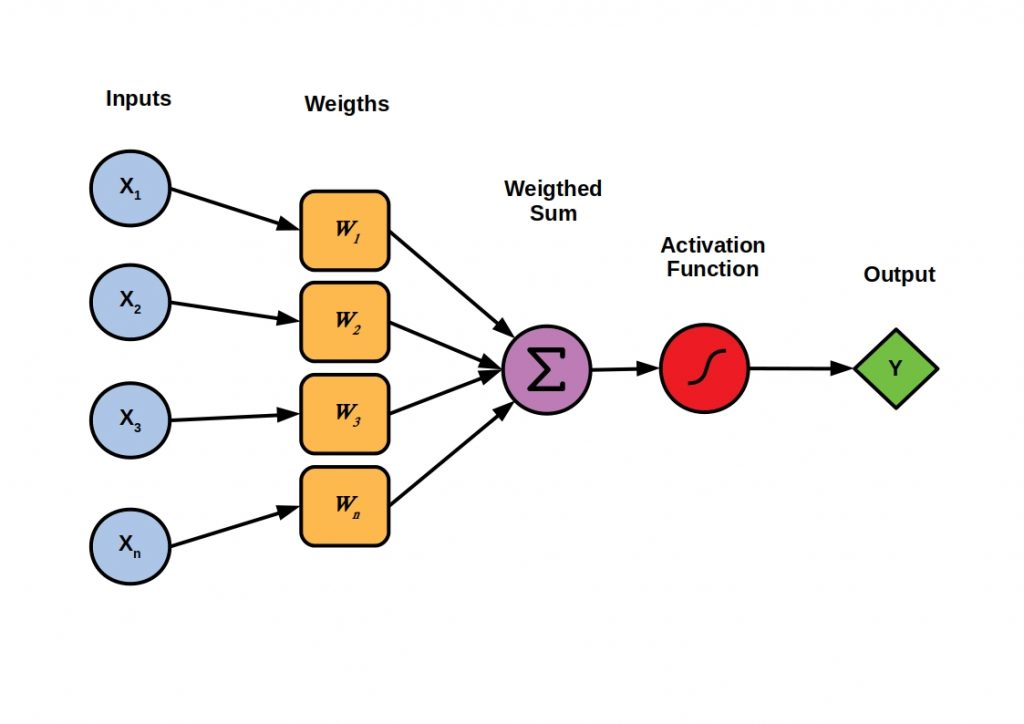
\includegraphics[width = 1 \textwidth]{Imagenes/Vectorial/Perceptrones.jpeg}
	\caption{Estructura del perceptrón (SilliconLotus, 2023)}
	\label{fig:perceptron}
\end{figure}

La primera imagen generada por Inteligencia Artificial fue en 1957, por el propio creador del perceptrón, Frank Rosenblatt, quien entrenó al propio perceptrón con una serie de imágenes de rostros humanos para que éste aprendiera e identificara un patrón y reprodujera una nueva imagen. La imagen fue generada a través de una matriz de puntos de luz que aunque no se asemejara a lo que realmente era una fotografía de una persona real, hizo que este fenómeno marca un antes y un después en el desarrollo de la inteligencia artificial generativa.\\

\textbf{¿Qué tipos de redes neuronales existen?}\\

La variedad de redes neuronales es considerablemente grande, y cada una de ellas se han ido desarrollando y diseñando para elaborar tareas específicas. De esta manera, las diferentes redes neuronales han ido adoptando diferentes arquitecturas para tratar diferentes tipos de datos.\\
Entre ellas, mencionaremos las más relevantes hoy en día y, analizaremos el funcionamiento de cada una para tener claro cuál es la más adecuada para el modelo de inteligencia artificial generativa de imágenes, haciendo una comparación entre unas y otras.

\subsection{Redes Neuronales Feedforward (FNN)}

Son un tipo de redes multicapa, que como hemos visto, están formadas por conjuntos de neuronas agrupadas en varios niveles o capas, en los que cada neurona está conectada y recibe señales de otras neuronas pertenecientes a la capa anterior, que a su vez, se encargan de transmitir información por señales a las neuronas de la capa posterior, en dirección a la salida de la red. De esta forma, las salidas de cada capa constituyen la entrada a la capa inmediatamente posterior (Russell y Norvig, 2010). En todo caso, las conexiones de la red fluyen exclusivamente en una sola y única dirección, de ahí el nombre feedforward, que traducido es hacia delante. Por norma general, la arquitectura típica que sigue una red neuronal multicapa consta de tres capas: capa de entrada, capa oculta y capa de salida (Berzal, 2018). \\

Sin embargo, cabe la posibilidad de que haya más de una capa de cada tipo, y cuando se da el caso de que la red consta de más de una capa oculta, la red se califica como profunda, traducida al inglés como \textit{deep neural network}. Concretamente, añadir más de una capa oculta a la red permite crear un modelo interno que reconoce patrones y proporciona un mayor rendimiento en la interpretación y estructuración de diferentes propiedades de objetos. Por ello, estas redes fueron diseñadas específicamente para resolver problemas de clasificación, regresión y por supuesto, como hemos visto, realizar reconocimiento de patrones.\\

\begin{figure}[h]
	\centering
	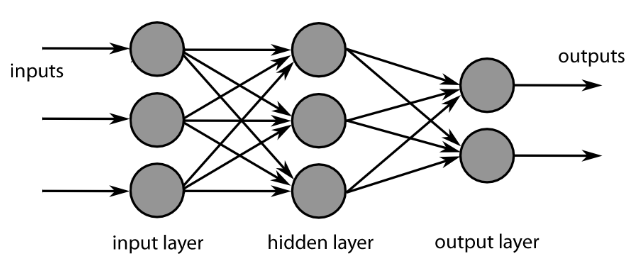
\includegraphics[width = 1 \textwidth]{Imagenes/Vectorial/feedforward.png}
	\caption{Red neuronal feedforward (Berzal,2018)}
	\label{fig:feedforward}
\end{figure}



\subsection{Redes Neuronales Recurrentes (RNN)} 

Como hemos visto, las redes neuronales \textit{feedforward} están habilitadas para que la información fluya en una sola dirección. Sin embargo, cuando se les proporciona una memoria, el resultado que se obtiene son las redes neuronales recurrentes, o \textit{Recurrent Neural Networks} (RNN) en inglés. El origen de estas redes se popularizó en 1982 por el físico americano John Hopfield, en las que se destacan por su comportamiento dinámico y estable (Berzal, 2018). \\

¿Y cómo es posible añadir memoria a las propias conexiones? Simplemente generalizando sus conexiones, es decir, alimentar a sus propias entradas o inputs con las salidas o outputs generados previamente por las conexiones anteriores provocando que el modo en el que fluyen las conexiones sea bidireccional. Es decir, incluyendo conexiones hacia atrás con las que se trabaja en una serie de pasos de tiempo, conocidos como \textit{timesteps}, donde se procesan los elementos de la secuencia uno por uno, manteniendo una memoria de los estados anteriores a medida que avanzan en la secuencia.\\

El entrenamiento de redes neuronales de estas características se realiza contando con diferentes algoritmos y técnicas, la más básica y conocida en este tipo de red neuronal es el algoritmo de propagación de errores (\textit{back-propagation} en inglés) formalizado en 1986 por Rumelhart, Hinton y Williams (Berzal, 2018). Este método, en concreto, consiste en aplicar un patrón a la primera capa de la red, el cual se va propagando hacia las capas superiores con el objetivo de generar una salida que se pueda comparar con la salida deseada y así poder calcular el error para cada neurona de la salida obtenida en función de los diferentes parámetros de la red. En otras palabras, cómo varía el error en relación con la variación de los parámetros de la red neuronal. Si a este fenómeno le sumamos la variable del tiempo, se obtiene la técnica de retropropagación a través del tiempo (\textit{backpropagatio}n through time, BPTT), en la que después de analizarse la secuencia completa, calcular el error y cambiar los parámetros para minimizar el mismo, se propaga el error a través del tiempo desde la última capa hasta la superior en cada paso de tiempo con el fin de que la red aprenda de las secuencias y mejore su predicción futura. 
Este método combinado con la técnica del gradiente descendente (en inglés \textit{gradient descent}) encargada de la optimización del error buscando los parámetros adecuados para poder reducirlo al mínimo es el modo de aprendizaje supervisado más popular que existe.  Aunque, como hemos visto anteriormente, no es el único, ya que coexiste con técnicas de entrenamiento como el aprendizaje no supervisado y el aprendizaje por refuerzo. \\

Así que podemos concluir en que las redes neuronales son idóneas para tareas de modelado de datos secuenciales y con dependencias temporales, como lo pueden ser el procesamiento de lenguaje natural, la generación de texto o la traducción automática, entre muchas otras.
\begin{figure}[h]
	\centering
	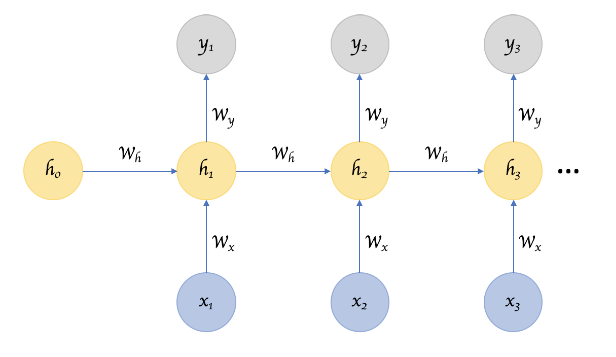
\includegraphics[width = 1 \textwidth]{Imagenes/Vectorial/recurrente.png}
	\caption{Red neuronal recurrente (Sensio, 2020)}
	\label{fig:rnn}
\end{figure}


\subsection{Redes Neuronales LSTM} 

Las redes neuronales Long Short-Term Memory surgen a partir de las redes neuronales recurrentes cuyo principal objetivo y propósito es ratificar el problema del desvanecimiento del gradiente o conocido en inglés como \textit{vanishing gradient problem} (Hochreiter y Schmidhuber, 1997). \\

En primer lugar y para entender en qué consiste este problema, es necesario saber qué es exactamente un gradiente y a qué nos referimos cuando hablamos del desvanecimiento del mismo. Un gradiente es una medida que determina la variación de una función con respecto al cambio que se produce en sus variables, ya sea en términos de optimización, rapidez o maximización de la función objetivo (Sanderson, 2017). \\

Matemáticamente, se puede entender como un vector multivariable cuyas variables son las derivadas parciales de dicha función. Se puede ver en el ejemplo de la figura \ref{fig:gradiente}. Geométricamente hablando, el gradiente indica la dirección en la que la función crece a mayor velocidad y, de esta manera, podemos concluir que el uso de algoritmo del  gradiente descendente (\textit{gradient descent}) se hace con el fin de ajustar los parámetros para reducir al mínimo la diferencia entre los valores obtenidos y los deseados. Un claro ejemplo de ello son los modelos de predicción, en los que se busca reducir dichas predicciones con respecto a los valores reales. \\

\begin{figure}[h]
	\centering
	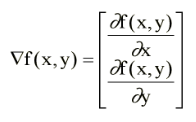
\includegraphics[width = 0.3 \textwidth]{Imagenes/Vectorial/gradiente.png}
	\caption{Función matemática del gradiente (Universidad Miguel Hernández, 2020)}
	\label{fig:gradiente}
\end{figure}

Ahora bien, cuando hablamos del desvanecimiento del gradiente (\textit{vanishing gradient problem}) nos referimos al fenómeno que ocurre en la propagación hacia atrás, cuando a medida que se va produciendo la propagación en capas cada vez más profundas, el gradiente va disminuyendo hasta llegar a ser tan pequeño que las capas superiores sean incapaces de aprender de manera efectiva. Este tipo de problema es común en redes conformadas por una gran cantidad de capas, dado que se disminuye exponencialmente a medida que va recorriendo cada capa hasta impedir que los pesos se actualicen de manera correcta y que puedan tener un aprendizaje lo suficientemente eficiente para ser capaces de resolver patrones complejos.
La solución a este problema se abordó introduciendo nuevos componentes a la red que ayudan y controlan el flujo de información de la red, consiguiendo aumentar la memoria del conjunto de la red al almacenar la información durante periodos más largos de tiempo. Los componentes principales son los siguientes:
\begin{itemize}
	\item \underline{Memory cells o celdas de memoria}: contienen la información relevante  y actualizada a lo largo del tiempo.
	\item \underline{Input gates o puertas de entrad}a: son las encargadas de controlar la cantidad de información que entra a las celdas de memoria.
	\item \underline{Forget gates o puertas de olvido}: seleccionan la información que debe ser eliminada de la celda, al no ser de utilidad.
	\item \underline{Output gates o puertas de salida}: su tarea radica en seleccionar la información de la celda que va a pasar a la siguiente capa de la red, basándose en el estado oculto actual.
\end{itemize}
 

De este modo, se consigue erradicar el problema del desvanecimiento del gradiente (\textit{vanishing gradient problem}) y se consigue procesar grandes secuencias de datos durante largos periodos de tiempo. Es especialmente útil en tareas que requieren capturar grandes dependencias de datos temporales, ejemplo de ello son el procesado y/o reconocimiento de lenguaje natural, en la traducción automática y en la generación de texto.\\

\begin{figure}[h]
	\centering
	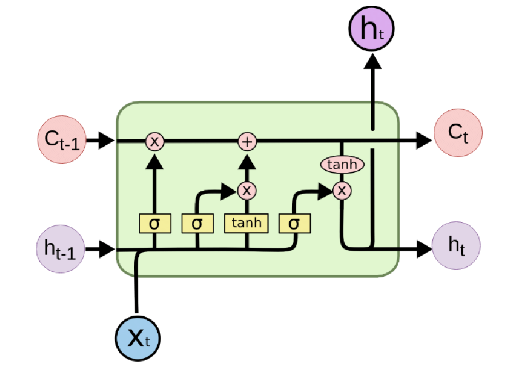
\includegraphics[width = 1 \textwidth]{Imagenes/Vectorial/lstm.png}
	\caption{Red neuronal Long Short Term Memory (Casallas, 2020)}
	\label{fig:lstm}
\end{figure}



\subsection{Redes Neuronales Convolucionales (CNN)}

Las redes neuronales convolucionales se introdujeron por primera vez en la década de los 50 por David Hubel y Torsten Wiesel cuando experimentaron con las neuronas biológicas, lo que le sirvió de inspiración a Kunihiko Fukushima en la década de los 80 para desarrollar el Neocognitron, una red neuronal que se conoce como la primera CNN. Este concepto fue cobrando forma con el paso de los años y el modelo tal y como lo conocemos hoy en día, fue obra de Yann LeCun en 1998 al introducir el aprendizaje a través de la técnica de backforwarding (Berzal, 2018).	\\

Las redes neuronales convolutivas están formadas por una secuencia de capas que podemos clasificar en tres tipos: capas convolutivas, capas de pooling y capas completamente conectadas.\\ 
\begin{itemize}
	\item \underline{Capas convolutivas}: suponen la capa principal de la red, y el papel que desempeña en el procesamiento de imágenes, es realizar la gran parte de los cálculos que se necesitan para extraer características de las imágenes. Para ello, hace falta la intervención de tres elementos principales: datos de entrada, un filtro y un mapa de características. 
	Los datos de entrada son el elemento que se trata de analizar, por ejemplo, en el caso de una imagen de color que estuviera compuesta por una matriz de píxeles en 3D, las dimensiones serían la altura, la anchura y la profundidad de la misma. 
	Por otro lado, el filtro o kernel, se trata de un detector de características, que va pasando por cada área de la imagen para identificar diferentes características, este proceso se denomina convolución. 

	El siguiente paso es representar mediante una matriz bidimensional de pesos, que al aplicarse en cada área calcula un producto escalar a partir de los píxeles de los datos de entrada y del filtro. El producto escalar se utiliza como input en la matriz de salida para que el filtro sea capaz de repetir el proceso por toda la imágen. La finalidad del filtro es ser capaz de distinguir diferentes patrones, como lo pueden ser texturas, bordes o figuras. 
	
	Finalmente, la suma de los diferentes productos escalares y el o los filtros utilizados, da como resultado final lo que se conoce como mapa de características. 
	
	Después de cada capa de convolución, se aplica una función de activación no lineal al mapa de características, a través de la ReLU (\textit{Rectified Linear Unit}). El fin de esta función es introducir no linealidad a la red, lo que le permite mejorar la complejidad entre las diferentes características (Krizhevsky et al., 2012). \\
	
\item	\underline{Capa de agrupación o pooling}: son capas dedicadas a reducir la dimensión del mapa a través de la disminución del número de parámetros de entrada.
	Comúnmente, se utilizan dos técnicas conocidas como \textit{max pooling} y \textit{average pooling}. \textit{Max pooling} consiste en seleccionar el pixel con mayor valor a medida que el filtro recorre la imagen para enviar el máximo a la matriz de salida, en cambio, average pooling lo que busca es calcular el valor medio del campo. El inconveniente que presenta esta capa es la gran pérdida de información que existe, sin embargo, presenta una gran ventaja a la hora de reducir la complejidad computacional y concentrarse en las características más importantes, lo que claramente, mejora el rendimiento del modelo y evita el riesgo de que se produzca un sobreajuste.\\ **explicar sobreajuste
	
	\item \underline{Capa totalmente conectada}: en las últimas capas de la red los nodos están conectados con los de la capa anterior para producir la salida final incorporando las características extraídas y aprendidas de los procesos realizados en las capas anteriores. Las capas totalmente conectadas se preocupan de realizar las funciones de clasificación de la imagen y de regresión para producir el resultado deseado (Krizhevsky et al., 2012). \\
	

\end{itemize}

	Las principales funciones y tareas que abarcan las redes neuronales convolucionales son el reconocimiento de imágenes identificando y detectando objetos, personas o animales; análisis de imágenes para diferentes propósitos, por ejemplo, médicos; reconocimiento facial; segmentación semántica; y por supuesto, generación de imágenes.\\
\begin{figure}[h]
	\centering
	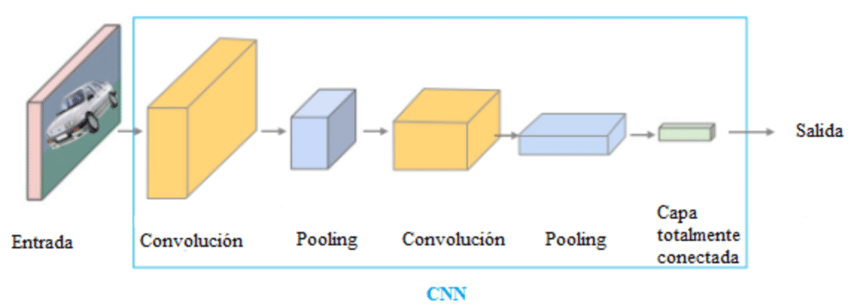
\includegraphics[width = 1 \textwidth]{Imagenes/Vectorial/cnn.png}
	\caption{Red neuronal convolucional (Andrade, 2021)}
	\label{fig:cnn}
\end{figure}

\subsection{Redes Generativas Adversarias (GAN)}

Las redes GAN, del inglés, Generative Adversarial Networks son un tipo de redes neuronales profundas relativamente novedosas, ya que surgieron en el año 2014 por primera vez por Ian Goodfellow y sus compañeros en la Universidad de Montréal (Goodfellow et al., 2014). \\

El funcionamiento de este tipo de redes involucra a dos redes neuronales diferentes, en las que cada una se encarga de realizar una tarea específica y “competir” contra la otra, para así, cada vez ir mejorando más los resultados obtenidos. \\

La primera red neuronal de este sistema se conoce como “Generador” y se encarga de producir y crear datos totalmente nuevos basándose en los datos aportados en el entrenamiento de la red. Se le asigna como entrada un vector de ruido y es responsable de crear datos que se asimilen a los datos originales. El entrenamiento del Generador es constante y siempre busca mejorar los resultados a medida que los va produciendo para alcanzar el máximo realismo posible. \\

La segunda red neuronal de la que se compone este sistema es el “Discriminador”, se dedica a analizar los resultados producidos por el Generador e identificar si son los reales o los creados por la red. A medida que va avanzando su entrenamiento, la capacidad del discriminador en distinguir entre un resultado real o falso dada una cierta entrada va mejorando cada vez más, haciendo que su predicción sea más certera. 
Un clásico ejemplo llevado a la vida real de esto puede ser el caso de un falsificador de billetes y un detective, en el que el primero tiene como muestra cierta cantidad de billetes e intenta replicarlos para que más adelante el segundo agente intente detectar la copia del original. A medida que pasa el tiempo, cada uno de los dos individuos van mejorando en su tarea llegando a un nivel de equilibrio. \\

Matemáticamente, el discriminador tiene que generar una salida, expresada como D(x), basándose en la probabilidad de que la entrada sea sintética o real, suponiendo que en cuanto más cercana a 1 sea, la entrada es original. Y por el contrario y dada una muestra aleatoria z en función de cierta distribución de probabilidad, el generador tiene que producir una muestra, expresada como G(z), que el discriminador tiene que clasificar como cercana a 0, produciendo una salida del tipo D(G(z)) en la que el generador tiene que intentar que su probabilidad se aproxime a 1, justo al contrario que el discriminador. Suponiendo que entre todas las muestras del modelo, una mitad son auténticas y la otra mitad son falsas, se tiene que alcanzar el conocido como equilibrio de Nash en el que las muestras del modelo son igual a los datos y en las que la probabilidad del discriminador es D(x) 0,5 para todo x (Berzal, 2016). \\

Por último, cabe destacar que para el entrenamiento de este tipo de red se utilizan los métodos del gradiente descendente (\textit{gradient descent}) y backpropagation, vistos en redes neuronales anteriores. \\

Este tipo de redes son ideales para tareas que requieren creación de datos realistas y artísticos, como lo pueden ser la generación de imágenes, de música o incluso, síntesis de voz. 

\begin{figure}[h]
	\centering
	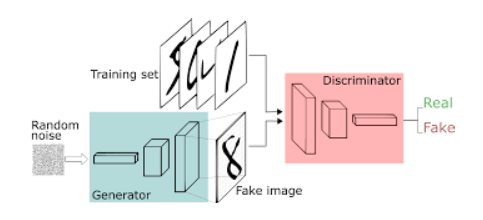
\includegraphics[width = 1 \textwidth]{Imagenes/Vectorial/gan.png}
	\caption{Red neuronal generativa antagónica (Franco, 2014)}
	\label{fig:gan}
\end{figure}


\subsection{Redes Neuronales Transformer}

Las redes neuronales Transformer son las más actuales tratadas en este trabajo, surgieron en 2017 a través del artículo “Attention is all you need” elaborado por Vaswani et al.. El artículo trata una mejora de las redes recurrentes y convolucionales conocidas introduciendo un mecanismo basado en la atención, en el que se consigue que algunas tareas se realicen en paralelo. Para ello, se parte de una entrada, la cual suele ser una frase u oración, mediante \textit{embedding} y se hace uso de dos componentes: codificador y decodificador. \\
\begin{itemize}
	\item \underline{Embedding}: es el primer bloque por el que está compuesto la red neuronal, su función es primordial para el manejo de los datos, ya que transforma el texto de la entrada en unos determinados vectores o tokens, los cuales son la representación numérica del valor inicial. \\
	\item \underline{Codificador o encoder}:  después del embedding de la entrada, el siguiente bloque es el codificador posicional cuya tarea es indicar a la red el orden de los diferentes elementos del vector, es decir, de las palabras en el texto. Esta función es esencial ya que la secuencia se procesa en paralelo, y de lo contrario, no se podrían concretar las posiciones de cada uno.\\
	
	A continuación, se encuentran conectados en secuencia un cierto número de los codificadores recién descritos. Cada codificador se compone de 4 elementos: el bloque residual, una red neuronal, otro bloque residual, y por último, un bloque atencional siendo el más importante de todos al encargarse de determinar la relevancia de cada uno de los \textit{tokens} para la frase junto a su asociación. Los restantes elementos se encargan de normalizar la entrada y la salida para poder seguir entrenando la red de forma productiva. \\
	\item 
	\underline{Decodificador o decoder}: cada codificador está conectado a un decodificador, que cumplen una composición similar, sino igual,  a  la explicada en los codificadores, es decir, cuatro elementos: dos bloques residuales, una red neuronal y un bloque atencional. A los que se le añaden dos elementos más en la estructura: un tercer bloque residual y un bloque atencional con enmascaramiento. \\
	
	Sin embargo, el funcionamiento difiere al de la estructura anterior. Se comienza con el bloque atencional con enmascaramiento que codifica las relaciones entre elementos atendiendo únicamente a palabras actuales y pasadas. Por otro lado, el bloque atencional del decodificador se conecta con el del codificador para establecer el orden de prioridad al que se debe prestar atención en la secuencia, sus valores son probabilidades entre 0 y 1 siendo el valor más alto el seleccionado. Por último, el comportamiento de los demás bloques cumplen la mismas funciones que en el codificador, incluyendo entre ellos, los bloques residuales, el bloque de codificación posicional y la salida en función del embedding.  \\
	
\end{itemize}


Por lo tanto, podemos afirmar que estas redes neuronales aprenden contexto y significado mediante el seguimiento de relaciones en datos secuenciales. Todo tipo de organizaciones utilizan estos modelos para conversión de secuencias, incluidas las de reconocimiento de voz y la traducción automática. Esta red neuronal procesa secuencias largas con cálculo paralelo, con el objetivo de reducir significativamente el tiempo de entrenamiento y de procesamiento.\\

A raíz de este modelo, surgen técnicas innovadoras como el aprendizaje por transferencia y la generación aumentada de recuperación (RAG). El objetivo principal es entrenar inicialmente los modelos de conjuntos de datos amplios y después refinarlos de manera precisa, utilizando conjuntos de datos más específicos. De este modo, se maximiza su utilidad y relevancia dentro de cualquier contexto.\\

\begin{figure}[h]
	\centering
	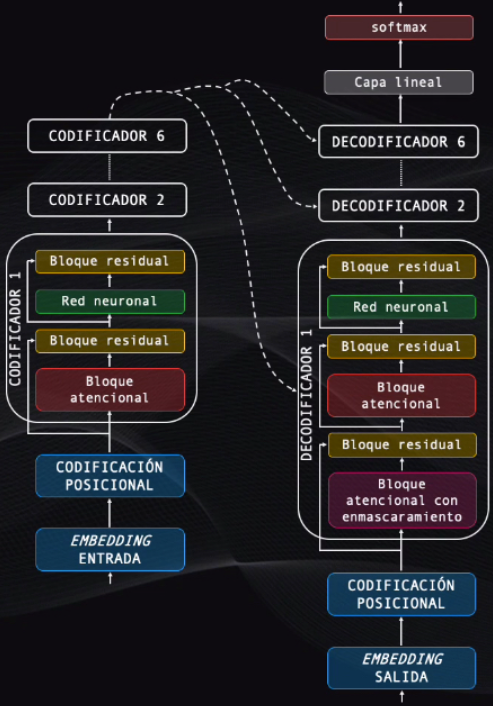
\includegraphics[width = 0.7 \textwidth]{Imagenes/Vectorial/transformer.png}
	\caption{Red neuronal Transformer(Sotaquirá, 2020)}
	\label{fig:transformer}
\end{figure}

Estos suponen sólo algunos ejemplos de los tipos de redes neuronales más comunes y ampliamente utilizadas. Cada tipo tiene sus propias características, fortalezas y debilidades, y es importante elegir el tipo adecuado según el problema específico que se esté abordando y el tipo de datos disponibles.\\

 \section{Stable Diffusion}

Como hemos visto, hay diferentes redes neuronales destinadas a la generación tanto de texto como de imágenes. En el caso de Stable Diffusion, el modelo de IA utilizado en nuestro proyecto, funciona con un modelo de difusión latente basado en CNNs y en Transformers. Ya visto el comportamiento y funcionamiento de ambas redes neuronales en apartados anteriores, analizaremos más en profundidad de qué manera se integran y complementan en el modelo que utilizaremos más adelante.\\


Stable Diffusion es un modelo de Inteligencia Artificial generativa cuya principal función es transformar el texto a imagen, aunque también presenta otras funciones asombrosas como la transformación de imagen a imagen o incluso lo más novedoso hasta el momento, transformaciones de texto a vídeo. Las empresas desarrolladoras hicieron una colaboración conjunta entre CompVis LMU, Runway y Stability AI y el lanzamiento finalmente se produjo a mediados de 2022. \\


\subsection{Funcionamiento interno de Stable Diffusion}

En principio, Stable Diffusion cuenta con un entrenamiento de más de 5 millones de imágenes proporcionado por el dataset Laion-5B que permite contar con una gran variedad de opciones de creación de imágenes, desde objetos, animales, paisajes y lugares, personas e incluso celebridades mundialmente conocidas con una calidad notable.\\ 

Comencemos entendiendo el funcionamiento del modelo de difusión latente, y para facilitar su explicación y comprensión,  lo diseccionaremos en dos partes: difusión y el espacio latente. El proceso de difusión que sigue la generación de una imagen es, en primer lugar y partiendo de las millones de imágenes del dataset mencionadas, se procede a añadir ruido gaussiano gradualmente a través de una serie de pasos hasta que las fotografías pierden todo valor y terminan siendo irreconocibles. Se podría decir que se comporta como una cadena de Markov, al ser el ruido gaussiano una variable aleatoria y al depender cada paso exclusivamente del anterior. Este primer método se conoce como difusión directa hacia delante o \textit{forward diffusion}.\\

\begin{figure}[h]
	\centering
	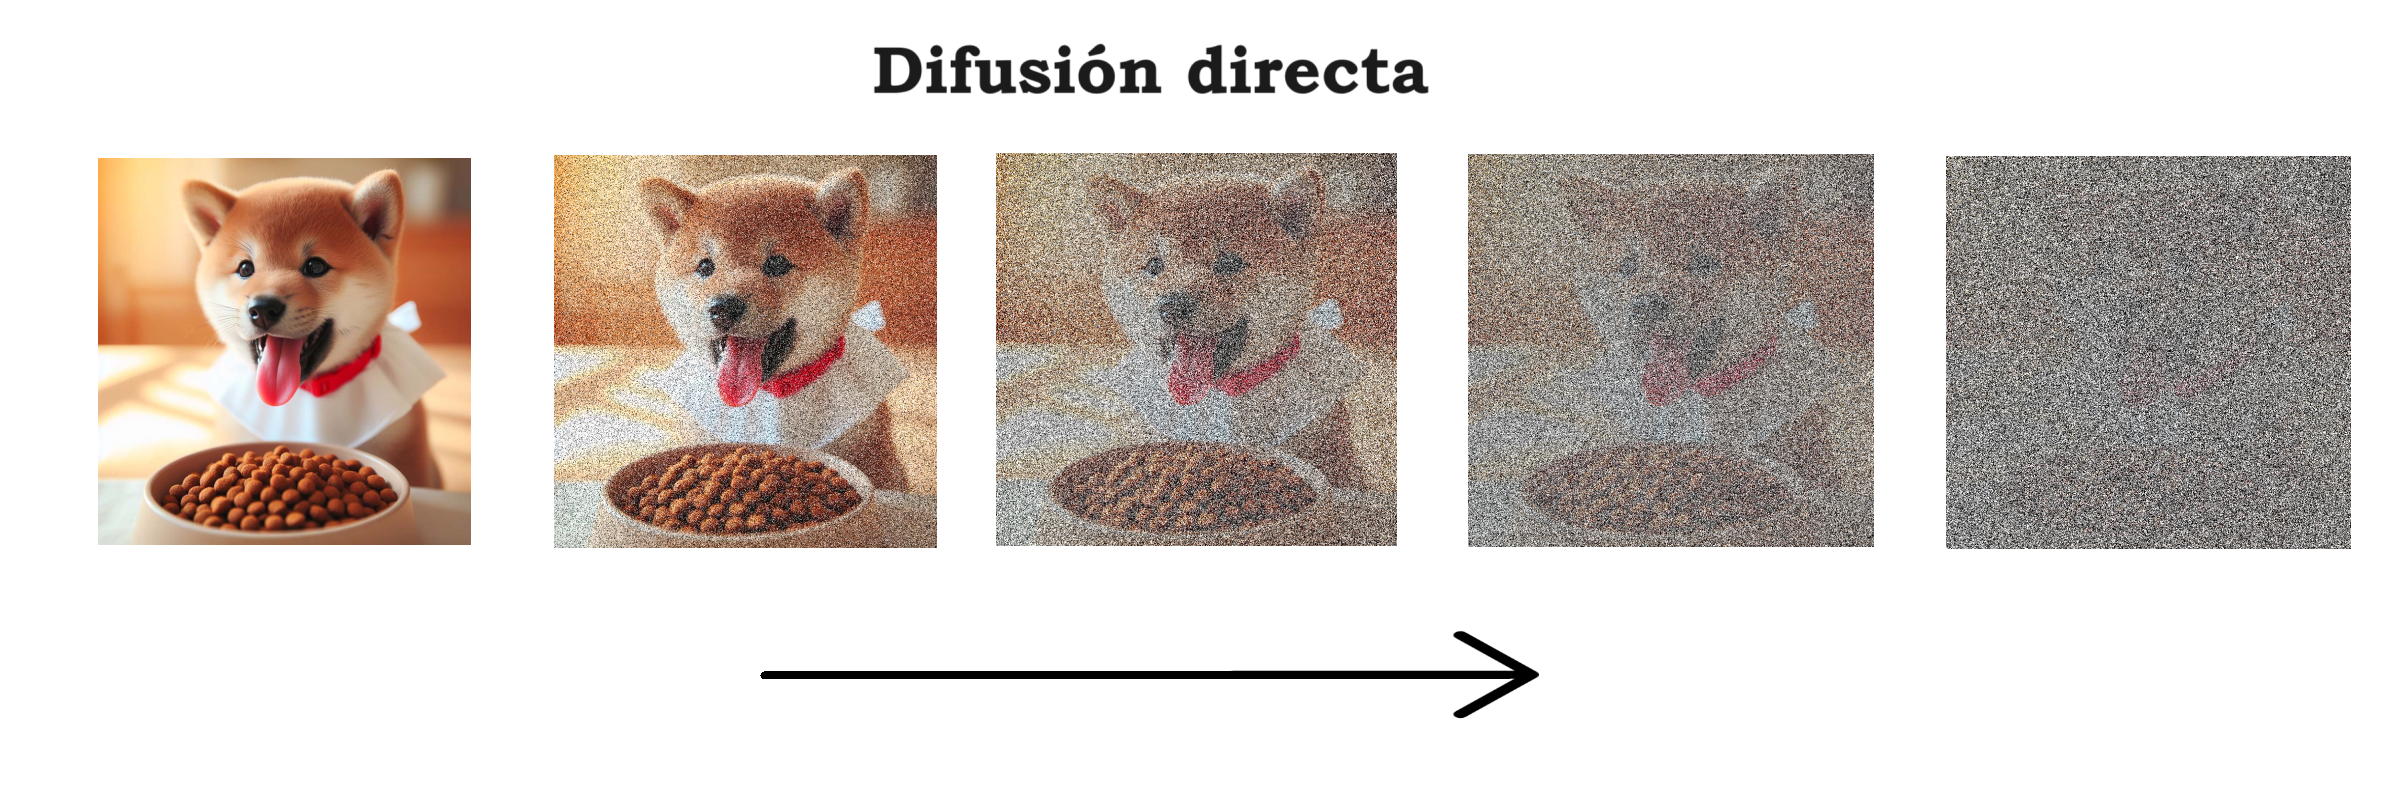
\includegraphics[width = 1 \textwidth]{Imagenes/Vectorial/difusiondirecta.png}
	\caption{difusión directa de una imagen de un cachorro de Shiba Inu comiendo}
	\label{fig:difusiondirecta}
\end{figure}

Así mismo, cuando se procesa una petición dado un \textit{prompt}, se parte de una imagen únicamente hecha de ruido aleatorio, es decir, un imagen sin nada relevante ni identificable en ella. Partiendo de esta imagen llena de ruido, se intenta revertir lo hecho anteriormente para volver a la imagen original quitando el ruido gradualmente. El ruido es aleatorio, y su aleatoriedad depende de un parámetro llamado \textit{seed} o semilla que asocia el ruido generado con un número aleatorio. Por lo tanto, si se repite la semilla se volverá a generar exactamente el mismo ruido y tendríamos como resultado una réplica de una imagen ya generada con esa misma semilla. Este proceso se conoce como difusión inversa y su objetivo principal es que el modelo aprenda a eliminar el ruido completamente. \\

\begin{figure}[h]
	\centering
	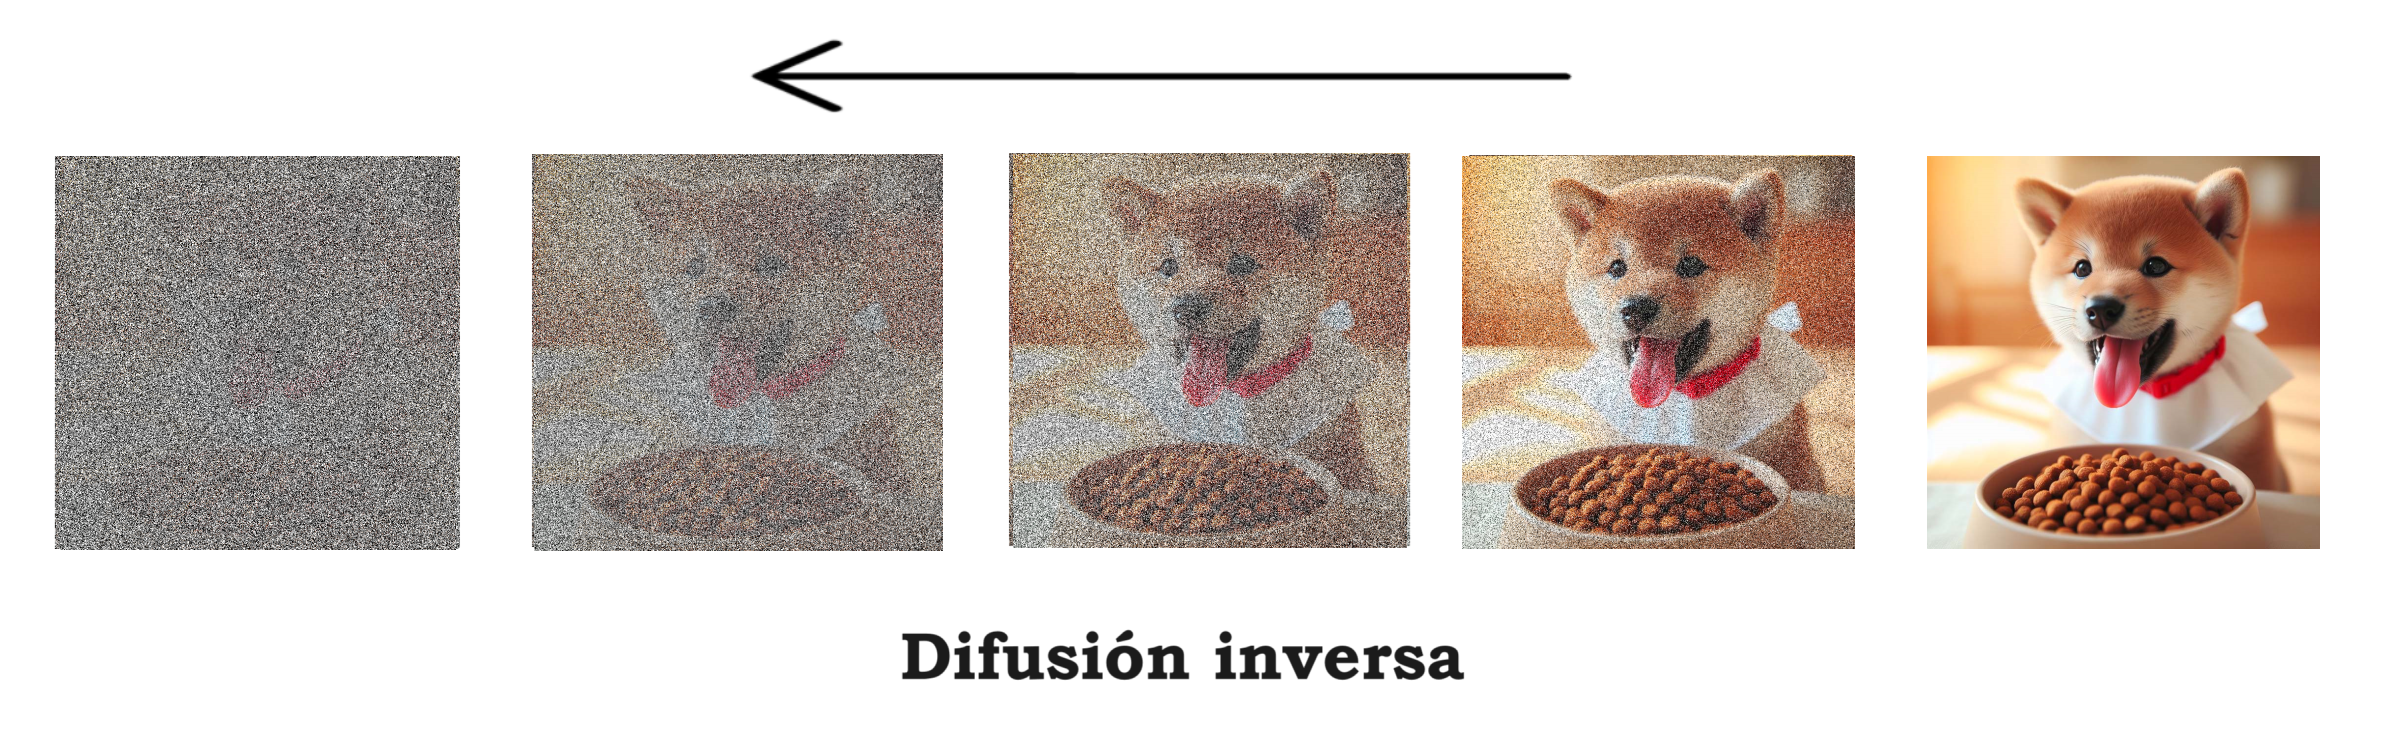
\includegraphics[width = 1 \textwidth]{Imagenes/Vectorial/difusioninversa.png}
	\caption{difusión inversa de una imagen de un cachorro de Shiba Inu comiendo}
	\label{fig:difusioninversa}
\end{figure}

Una vez tenemos la imagen llena de ruido y la forma de calcular el ruido que hay en cada imagen para poder eliminarlo, se empieza el proceso al que llamamos \textit{sampler} o muestreo. Aquí es cuando entra un componente importante llamado \textit{noise scheduler}, cuya función es determinar la cantidad de ruido que se debe suprimir en cada paso para alcanzar la forma óptima y que se puedan evitar cambios bruscos entre paso y paso, que sea de forma gradual y que los detalles se vayan puliendo conforme la imagen vaya cobrando más forma. El proceso de muestreo se repite la cantidad de \textit{steps} o pasos especificada por el usuario. Y de esta manera, concluimos con el primer componente del modelo de difusión latente: la difusión.\\ 

Pasemos a la segunda pieza del puzzle: el espacio latente. El proceso de difusión, por lo que hemos podido ver, es un proceso algo lento y costoso al tener que trabajar con los píxeles de una imagen. Si tenemos una imagen en color con la escala RGB de 512x512 píxeles, estamos hablando de una multiplicación de 3x512x512, es decir, un espacio de casi 80 mil dimensiones. Para solucionar este problema, se trabaja con el espacio latente que trata de reducir la imagen a una escala de 64x64 píxeles, asegurando mayor velocidad y una menor carga de trabajo al trabajar, de esta forma, con unas dimensiones más pequeñas de apenas 12 mil. 

\begin{figure}[h]
	\centering
	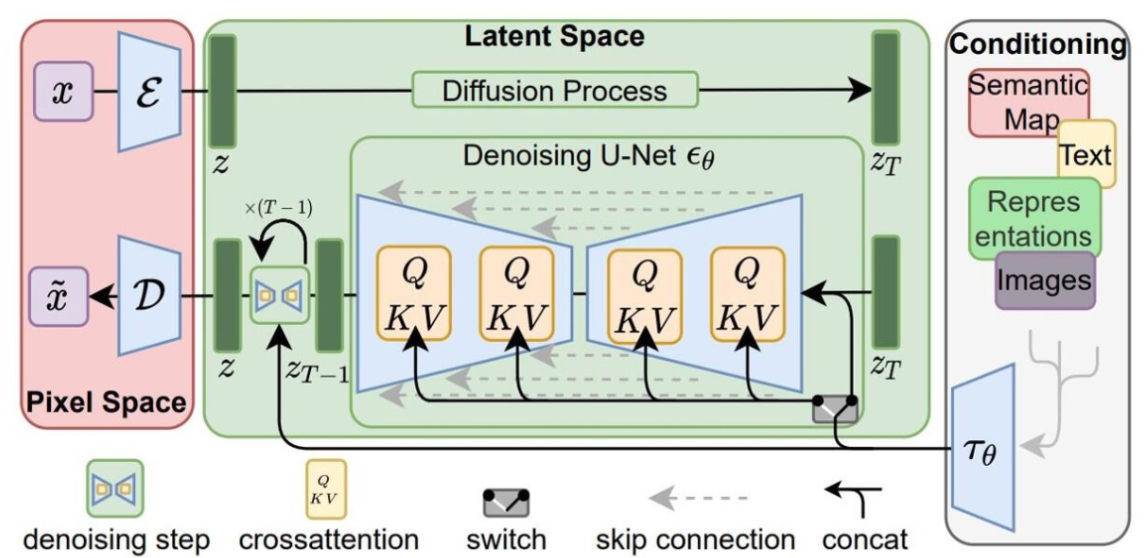
\includegraphics[width = 1
	\textwidth]{Imagenes/Vectorial/espaciolatente.png}
	\caption{Representación gráfica del proceso de conversión al espacio latente}
	\label{fig:latentspace}
\end{figure}

Ahora que entendemos el propósito y el funcionamiento de las dos variables del modelo de difusión latente, profundicemos más en cómo se lleva a cabo cada uno de estos dos procesos y qué mecanismos se utilizan para ello. El modelo se compone principalmente de 3 componentes: un codificador de texto basado en redes transformer, una red U-Net compuesta de dos redes ResNet y un autocodificador variacional (VAE).\\
\begin{itemize}
	\item \underline{Codificador de texto basado en Transformers}: para producir la imagen que deseamos, previamente es necesario escribir una descripción detallada de la imagen y es por tanto, el primer paso. Este texto que le introducimos al modelo se conoce como \textit{prompt} y es de lo que se encarga de procesar el codificador de texto.  Lo primero que realiza el \textit{text-encoder} de Stable Diffusion es a través de un modelo llamado CLIP (\textit{Contrastive Language-Image Pre-Training}) que se encarga de ofrecer una descripción detallada de las imágenes a través de su propio tokenizador. El siguiente paso y como ya hemos visto en apartados anteriores, el transformer se encarga de realizar la fase de \textit{embedding} en la que se transforman las palabras de texto en \textit{tokens} que la red neuronal pueda entender y manejar, para que después, a través del método de \textit{self-attention}, se decida qué palabras son las que más relevancia tienen.\\ 
	
	Además, Stable Diffusion ha añadido a esto una pequeña variación y mejora que añade a esta última técnica, otra llamada \textit{cross-attention} (o atención cruzada) con la que se permite crear relaciones entre los diferentes \textit{embedding} y mejorar la precisión del resultado. Por ejemplo, si el \textit{prompt} pedido es “unas flores pequeñas sobre una bicicleta azul”, solamente con la técnica de \textit{self-attention} podría procesarse una imagen que fuera “una flor azul sobre una bicicleta pequeña”, lo cual es válido para esa arquitectura pero no es lo que el usuario ha pedido. En cambio, con la ayuda de la técnica de atención cruzada se crean relaciones que tienen más a menos distancia, en la que en este ejemplo la relación flores con azul tiene más distancia que la relación de flores con pequeña, y por tanto, es esta última la que se utilizaría al tener más relación y menos distancia.\\
	\item \underline{Red neuronal U-Net}: es una red neuronal convolucional entrenada para identificar e intentar predecir la cantidad de ruido contenida en una imagen. Consta de un codificador y un decodificador en los que cada uno de estos componentes son, a su vez, bloques ResNet, que son redes convolucionales profundas compuestas por una gran cantidad de capas. La función del codificador se basa en reducir la calidad de la resolución de la imagen mientras que  la función del decodificador es la contraria, generar la imagen en la máxima resolución posible. Entre ambos componentes se añaden conexiones de acceso directo para evitar la pérdida de información importante. Al final, lo que se pretende conseguir es que la red U-Net consiga determinar el ruido para posteriormente, poder conseguir una representación libre de ruido en la imagen final.\\
	
	\begin{figure}[!htb]
		\centering
		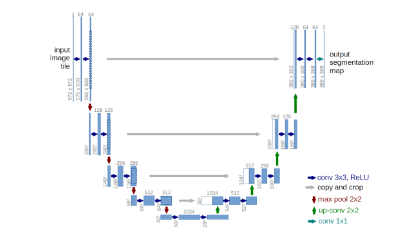
\includegraphics[width = 1
		\textwidth]{Imagenes/Vectorial/u-net.png}
		\caption{Arquitectura de una red U-Net}
		\label{fig:unet}
	\end{figure}
	\item \underline{Autocodificador variacional VAE}: es un tipo de red neuronal que al igual que las redes U-Net consta de dos componentes: un codificador y un decodificador, sin embargo sus funciones distan mucho las unas de las otras. El primer componente del autocodificador variacional se encarga de uno de los primeros pasos que realiza Stable Diffusion, que es convertir el espacio de píxeles de la imagen en un tensor dentro del espacio latente de menores dimensiones sustrayendo las características más relevantes de la imagen original y comprimiéndolas en el tensor latente. Y al final del proceso de difusión, se parte del tensor del espacio latente con el que se ha trabajado, para transformarlo en la imagen final generada en una escala de 512x512 píxeles.
	
\end{itemize}

\begin{figure}[!hbt]
	\centering
	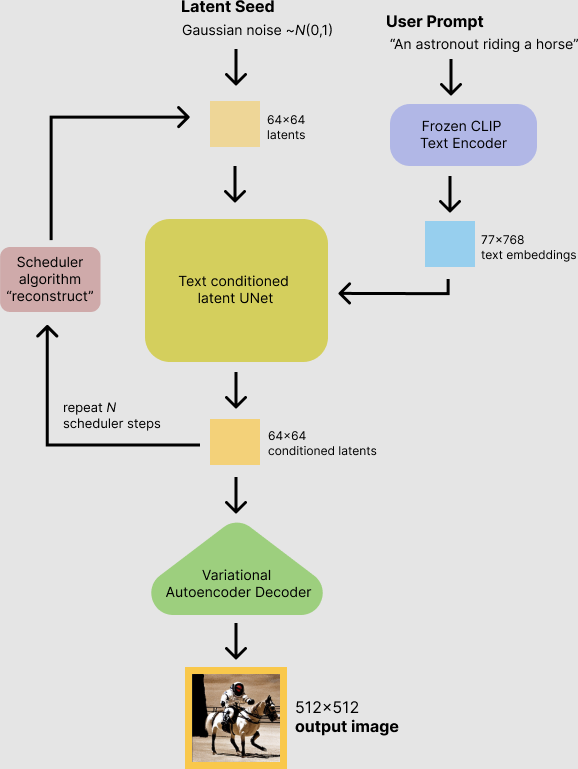
\includegraphics[width = 0.9
	\textwidth]{Imagenes/Vectorial/representacionvisualSD.png}
	\caption{Representación gráfica del funcionamiento de Stable Diffusion}
	\label{fig:sd}
\end{figure}

\subsection{Herramientas de Inteligencia artificial generadoras de imágenes}

\subsubsection{DALL-E}

Cita 1 \cite{russell2016artificial}

Cita 2 \citep{goodfellow2014generative}

Cita 3 \citet{hochreiter1997long}

Cita 4 \cite{krizhevsky2017imagenet}

Cita 5 \citep{berzal2019redes}

Cita 6 \citet{berzalmodelos}

Cita 7 \cite{rosenblatt1958perceptron}

Cita 8 \citep{gonzalez1995redes}


\subsubsection{Midjourney}
\chapter{Generación de imágenes con Stable Diffusion}
\label{cap:genimgsia}

\section{Elección del modelo}

Como hemos podido ver, Stable Diffusion es una herramienta potente y eficaz con una buena estructura que cuenta con una gran base de datos en la que podemos encontrar una inmensa variedad de imágenes. Estas características la convirtieron en nuestra elección final, pero veamos más en profundidad el proceso de elección de esta Inteligencia Artificial generativa en comparación con la amplia variedad de las que hay presentes actualmente en el mercado. 

En primer lugar, para entender nuestra elección es necesario poner en contexto el gran abanico de posibilidades de IAs generativas que hay hoy en día, sus prestaciones, características, y sobre todo, su accesibilidad. 

Las IAs generadoras de imágenes más potentes del mercado y las que consideramos para desarrollar la base de nuestro trabajo son Midjourney, DALL-E, Leonardo AI y Stable Diffusion, todas ellas producen unos resultados bastante satisfactorios. Sin embargo, descartamos rápidamente las dos primeras: Midjourney producida por un laboratorio independiente y,
DALL-E producida por la famosa empresa creadora de ChatGPT, OpenAI. El motivo fue que al ser ambas de pago, no podíamos tener acceso a su modelo de forma tan amplia como las demás, siendo prácticamente imposible acceder a ellas y mucho menos a poder entrenarlas. 

Para acceder a los modelos utilizamos Hugging Face, la plataforma  que cuenta con una amplia gama de bases de datos de todo tipo y de modelos de IA generativa de texto a imagen, imagen a imagen, imagen a texto y un largo etcétera. Intentamos buscar modelos de ambas en la plataforma sin éxito ya que lo máximo que encontramos eran imitaciones o pequeñas demos que no alcanzaban el nivel de calidad requerido. \\


Leonardo AI sí que es una opción algo más accesible ya que la plataforma sí que cuenta con un plan gratuito que te deja probar el modelo con una limitación de 150 imágenes a generar al día, lo cual está muy bien. Además, la calidad es bastante buena y permite ajustar gran variedad de parámetros, como por ejemplo, el número de imágenes que deseamos que se generen al mismo tiempo, el estilo, la paleta de colores que deseamos, tamaño e incluso la resolución. El inconveniente era la accesibilidad al modelo y la información sobre este mismo, ya que era escasa y en Hugging Face no había acceso. En comparación con Stable Diffusion, la incertidumbre era mucho más alta y había muchísimas limitaciones a la hora de utilizarlo. \\

Todo ello nos llevó a elegir Stable Diffusion rápidamente, una herramienta open source, es decir, de código abierto que nos facilita mucho el entrenamiento de personas para obtener imágenes personalizadas de forma rápida y con alta calidad. Además, sus diferentes versiones nos permitían explorar aún más a fondo el modelo y saber cuál era el que encajaba con las características que presentaban las prestaciones de nuestros equipos. Stable Diffusion resultó ser la candidata ideal para que la creación de imágenes destinadas a  los libros de vida fuera lo más sencilla, familiar y creativa posible. \\

Ahora expuestos todos los motivos de elección de Stable Diffusion, tanto en comparación con otras redes neuronales vistas en el Capitulo 2 como en comparación con otros modelos de IA Generativa, expondremos cómo implementamos la herramienta a lo largo de todo el trabajo y las dificultades a las que nos enfrentamos durante el proceso. \\

\section{Entrenamiento con Stable Diffusion}

\subsection{Versiones y métodos de entrenamiento}

Stable Diffusion cuenta, hasta el momento, con 3 grandes versiones que, paulatinamente, han ido mejorando la calidad en las imágenes generadas. Todas ellas son totalmente gratuitas y de libre acceso, la primera versión que se presentó fue Stable Diffusion 1 (en sus variaciones 1.4 y 1.5), seguida por Stable Diffusion 2 (con sus respectivas variaciones 2.0 y 2.1) y por último, Stable Diffusion XL (que cuenta con su variación XL Turbo). 

La diferencia principal entre las dos primeras versiones es el tamaño de resolución de las imágenes ya que las primeras versiones trabajaban en un espacio de 512x512 píxeles y en la versión 2 dicho tamaño aumentó a 768x768. Además, se introdujeron algunas correcciones y mejoras como la técnica de inpainting, que se trata de la restauración de algunas partes de la imagen mejorando la calidad y los detalles de la misma o incluso, reemplazando ese área por lo especificado por el usuario en el prompt.

Con la última versión Stable Diffusion XL, se generan imágenes con una calidad excepcional, lo que supuso una gran mejora en el modelo al contar con un dataset mucho más extenso. El inconveniente con la versión XL, en nuestro caso, era la limitación de que requiere una tarjeta gráfica demasiado potente, con la que, por desgracia, no contamos en nuestro equipo. 

Respecto a la versión 2, si bien es verdad que no requiere tanta GPU como la versión XL, sí que requiere más que en la primera versión, al ser las imágenes con mayor resolución y, viendo la comparación en la calidad que presentaban los resultados de ambas, optamos por utilizar la versión 1.5 ya que era la que mejor se adecuaba a nosotros en términos de calidad y tiempo.


Ahora bien, existen varios métodos a través de los cuales se puede utilizar esta herramienta y hemos probado sus funcionalidades de diferentes maneras. En primer lugar, se puede utilizar mediante código escrito en Python a través de Google Colab, ya que la plataforma ofrece cuadernos en los que se trabaja de manera online y que además, proporciona una GPU en la nube a la que Google te da acceso. En concreto, esta GPU es la T4, que es la única opción que nos deja Google entre las que hay (A100 GPU, L4 GPU, V100 GPU) ya que se conoce que las demás son de pago. Otra alternativa es mediante la propia página de Stable Diffusion, que ofrece una demo para utilizar esta avanzada versión. Por último, ejecutar el modelo en local, consiguiéndolo descargar en la página Hugging Face, que incluye multitud de modelos de todo tipo, bases de datos, librerías y licencias para descargar y utilizar, por lo que hemos podido comprobar,presenta muy buenos resultados.\\

El hecho de probar un modelo de inteligencia artificial en un servidor no es concordante con nuestros objetivos del proyecto, puesto que necesitamos entrenar un modelo e incluirlo en una aplicación, de manera que el usuario pueda interactuar y conseguir imágenes personalizadas en un tiempo aceptable, por ello descartamos la opción de utilizar la demo que se encuentra en la página de Stable Diffusion. \\

Una vez que tenemos el modelo de generación de imágenes elegido, se debe ejecutar en nuestro ordenador y ver cuál es el rendimiento real. Esto quiere decir que la imagen debe generarse de manera correcta y sin deformaciones, y debe incluir todos los elementos solicitados en la descripción introducida. Además, debe realizar esta generación en un tiempo adecuado.\\

Para ello, el proceso más óptimo y que finalmente elegimos llevar a cabo tras gran cantidad de pruebas es, en primer lugar, realizando el entrenamiento de imágenes personales a través de la plataforma de Google Colab en internet y en segundo lugar, para la generación de imágenes desde nuestro ordenador optamos por la instalación de una interfaz, llamada NMKD Stable Diffusion GUI. Esta herramienta nos permite ejecutar localmente cualquier modelo de generación de imágenes a partir de texto, e incluso permite aceptar imágenes como input, es decir, generaciones de tipo imagen a imagen. 

El principal de los objetivos que establecimos en la realización del proyecto era generar imágenes personalizadas del paciente en cuestión, y para ello es estrictamente necesario entrenar el modelo elegido.

Como se ha dicho anteriormente, el método elegido fue un cuaderno en Google Colab mediante Dreambooth,  un modelo de generación de aprendizaje profundo, y que fue desarrollado en 2022 por un grupo de investigadores de Google Research y la Universidad de Boston.  Este modelo nos permite añadir capas de entrenamiento a la inteligencia artificial para que reconozca objetos concretos. Esto es muy importante, porque es el mecanismo que consigue mejores resultados y con una velocidad aceptable, que era la utilización que queríamos otorgarle. Por consiguiente, podemos decir que la misión de esta tecnología es la de poder entrenar a modelos de inteligencia artificial para personalizarlo según tus necesidades.

\subsection{Requisitos en las imágenes de entrenamiento}

Para realizar el entrenamiento de una forma correcta, lo primero que tenemos que tener claro es  el elemento o token al que queremos dar una identidad. Por ejemplo, si seleccionamos una persona, debemos elegir unas imágenes en las que aparezca, de tal manera que, tras el entrenamiento, la IA pueda identificarla. 

Lo ideal es que se elija un número considerable de fotografías, a partir de 10, las cuales tienen que cumplir ciertas características. Deben ser fotografías de buena calidad, bajo diferentes ángulos, escenarios y luces, se recomienda que como mínimo hayan 1 o 2 fotografías en las que la persona aparezca de perfil, mostrando 3 cuartos de la cara, de frente y si es posible que en alguna esté sonriendo (para que la IA pueda reconocer la expresión), de cuerpo entero, cintura para arriba y del rostro de cerca. Además, es importante que la ropa no sea siempre la misma, sino al ser así, el modelo podría interpretar como que la ropa forma parte de la persona y siempre se la generaría con la misma, lo cual no queremos que ocurra. Idealmente, las fotografías deberían alternar la luz y estar hechas tanto en interiores como en exteriores. Por último y esto es fundamental, estas deberán tener un tamaño igual o mayor a 512 x 512 píxeles, y deberán llamarse exactamente de la misma manera, con el identificador del token al que hagamos referencia. Además, es preferible que todas las imágenes tengan la misma extensión, ya sea .jpg o .png. 

\subsection{Procedimiento de entrenamiento}

En el ejemplo de la figura \ref{fig:datasethoyeon}  elegimos como persona de entrenamiento una que no fuese reconocida por nuestro modelo (al contar con un dataset de 5 mil millones de imágenes, ya de por sí reconoce a varias personas famosas sin necesidad de entrenarlas). En este caso, se trata de una actriz coreana llamada Jung Hoyeon, y el token que le otorgamos, como se puede ver, respondía bajo el nombre de ``sqgkhoju''. Lo ideal, es que la etiqueta no sea nombrada bajo una palabra que el modelo pueda reconocer, es decir, que el token no tenga significado. Si por un casual llamasemos al token ``mujer'', seguramente la IA no logre ni identificar ni asociar a la persona que hemos entrenado, y probablemente acabe generando la imagen de una mujer que no existe, que es justamente lo que queremos evitar. \\

\begin{figure}[h]
	\centering
	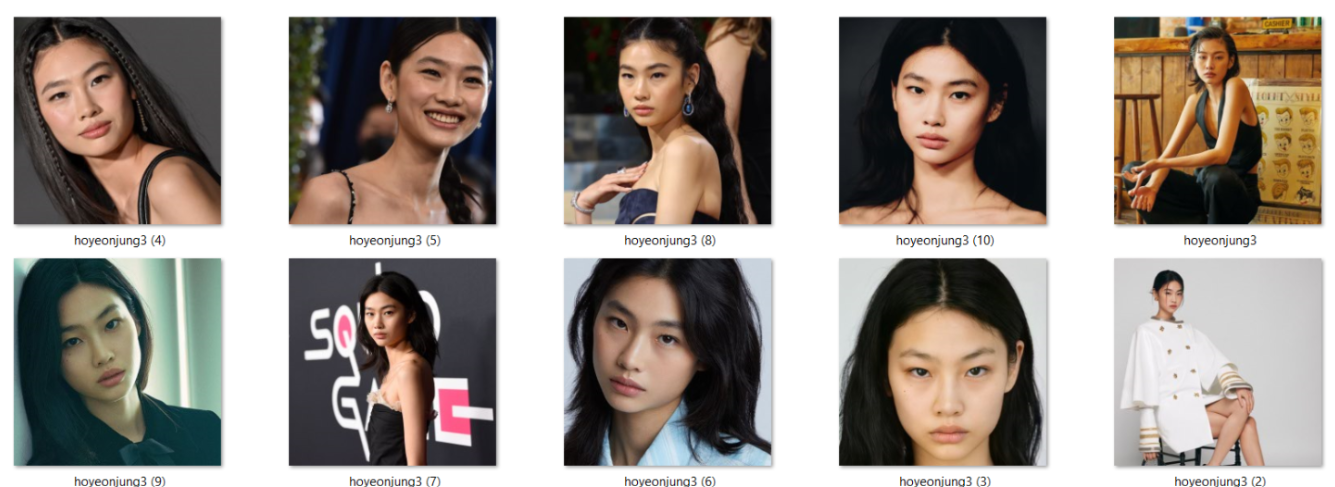
\includegraphics[width = 1
	\textwidth]{Imagenes/Vectorial/datasethoyeon.png}
	\caption{Dataset seleccionado para el entrenamiento de personas con Lora}
	\label{fig:datasethoyeon}
\end{figure}

Una vez que las imágenes cumplan con todos los requisitos, debemos utilizar el código abierto en la plataforma Google Colab para realizar el entrenamiento. 
El proceso que sigue el cuaderno es muy sencillo, en él sólo hace falta seguir una serie de pasos para completarlo. El primero es conectar el cuaderno a una cuenta de Google, para que se pueda guardar en el Drive asociado a esa cuenta una carpeta llamada ``Fast-Dreamboot'', en la que se guardaran todos los archivos que se generen durante el proceso. El siguiente paso es instalar las dependencias necesarias para ejecutar el código en python, seguido de establecer un nombre a la sesión en la que estamos trabajando, para que en un futuro cuando se hagan entrenamientos diferentes, se puedan distinguir unos de otros. En este paso se crea una carpeta llamada Sessions dentro de la carpeta mencionada recientemente. A su vez, esta carpeta contendrá otra bajo el nombre de la sesión que hayamos especificado en el cuaderno, y es ahí donde se guardaran todos los archivos que se creen en la ejecución. 

A continuación, es turno de subir las imágenes previa y cuidadosamente seleccionadas. Ya sea seleccionándolas directamente desde la carpeta en la que las tengamos guardadas en local, o habiéndolas subido previamente a una carpeta de la cuenta de Google Drive, y proporcionar la ruta en la que están en la celda del cuaderno habilitada para ello. 

El último paso, y uno de los más importantes, consiste en establecer algunos parámetros con los que se va a entrenar al modelo. El más importante y el único que nosotros hemos modificado, entre todos los que hay, es el número de steps. De modo que, en cuanto mayor sean, más tiempo tardará en generarse el archivo. Normalmente, se tardaba unos 20 o 25 minutos en terminar de entrenarse, lo cual hemos considerado que es bastante rápido. En el ejemplo de la figura \ref{fig:dreambooth} se puede ver la ejecución del progreso de entrenamiento en el que para una cantidad de 2000 pasos lleva 21 minutos y 36 segundos. 

Tras la finalización, se creará un archivo de alrededor de 2 giga bytes, que contendrá el modelo de Stable Diffusion 1.5, con una capa de entrenamiento más, puesto que incorporará el elemento deseado. Con esto ya tendríamos un elemento de inteligencia artificial personalizado.\\

\begin{figure}[h]
	\centering
	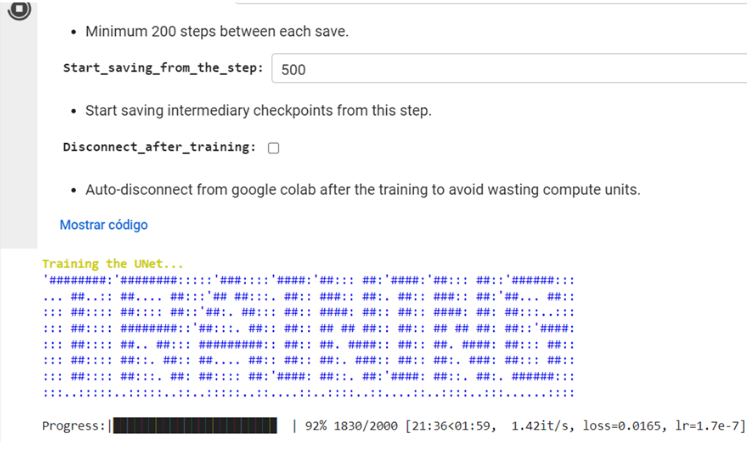
\includegraphics[width = 1
	\textwidth]{Imagenes/Vectorial/dreambooth.png}
	\caption{Procedimiento del entrenamiento mediante Dreambooth}
	\label{fig:dreambooth}
\end{figure}

Este archivo, en formato ckpt, se podrá utilizar en la aplicación NMKD SD GUI más adelante para generar imágenes, y contendrá el elemento entrenado bajo el token seleccionado. Si posteriormente se pretende incluir elementos al modelo ya entrenado, también se puede realizar empezando de nuevo el proceso de entrenamiento y utilizando de base el archivo en extensión ckpt anterior. Cuando se realice este segundo entrenamiento, se podrán generar imágenes acerca de ambos elementos, lo cuál es muy útil para nuestros objetivos, ya que en un mismo modelo enfocado a un paciente, debe haber múltiples elementos. Sin embargo, más adelante veremos que este último aspecto ha supuesto uno de los grandes fallos que experimenta el modelo en cuanto a múltiples capas de entrenamiento. \\

Un aspecto muy importante a tener en cuenta, es que tras la realización de múltiples pruebas, los resultados óptimos que hemos obtenido ha sido seleccionando un conjunto de datos formado por 10 imágenes, y con 2400 pasos de entrenamiento. 
%En la tabla \ref{tab:resultadosentrenamiento}\\



%\subsection{Entrenamiento con Dreambooth}
%\begin{table}
%	\centering
%	\begin{tabular}{c|c|c|c}
%		\textbf{Intento} & \textbf{Número de imágenes} & \textbf{Número de pasos} & \textbf{Veredicto} \\
%		\hline\hline
%		1 & 20 & 4000 & 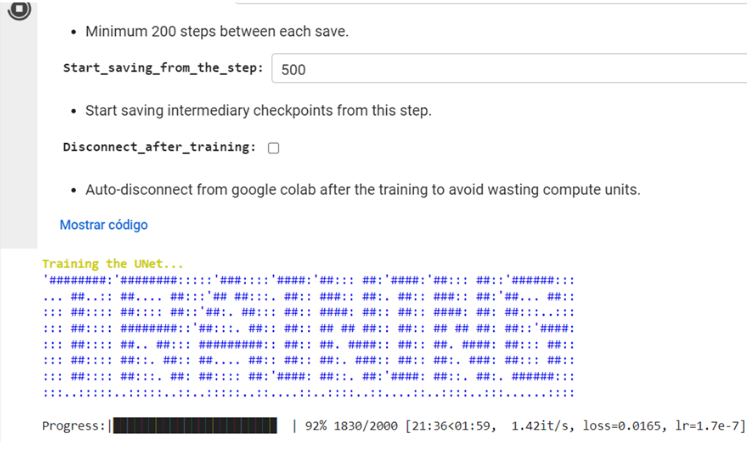
\includegraphics[width = 0.3
%			\textwidth]{Imagenes/Vectorial/dreambooth.png}\\
%		2 & 20 & 3000 & \\
%		3 & 15 & 3000 & \\
%		4 & 15 & 2000 & \\
%		5 & 10 & 3000 & \\
%		6 & 10 & 2400 & \\
%		\hline
%	\end{tabular}
%	\caption{Tabla de resultados obtenidos de entrenamiento}
%	\label{tab:resultadosentrenamiento}
%\end{table}


Hemos querido poner a prueba, no sólo las capacidades del modelo de entrenar a personas, ya que hemos podido comprobar sus puntos fuertes y débiles en la generación de seres humanos (los cuales podremos ver más adelante), sino de elementos que consideramos que también son de suma importancia a la hora de representar recuerdos: animales y lugares. \\

El objetivo de entrenar al modelo con lugares es que estos no se encuentren en la base de datos de imágenes de Stable Diffusion, puesto que de ser así, no tendría sentido realizar el entrenamiento. De este modo, podremos lograr que el paciente pueda rememorar sitios emblemáticos en su memoria y que las imágenes generadas que emulan recuerdos consigan ser aún más personales. Por ejemplo, el parque de su vecindario, la casa de sus padres o incluso, su propio salón. 

Las primeras pruebas que realizamos sobre un lugar se trataba de un edificio característico, que por supuesto no estaba incluido e el modelo previamente. Hablamos de la basílica de Colmenar Viejo, Madrid. Las imágenes seleccionadas estaban hechas desde diferentes ángulos, alturas, luces y lejanías. En la figura \ref{fig:datasetcolme} se pueden apreciar las características que reúnen las fotografías en cuestión y el token otorgado.

Además, quisimos comprobar si el número de imágenes y steps establecidos para las personas, producía resultados igual de satisfactorios para lugares. Y efectivamente, corroboramos la hipótesis de manera airosa. Ejemplos de ello, lo podemos ver en el apartado siguiente de Resultados.  

\begin{figure}[!htb]
	\centering
	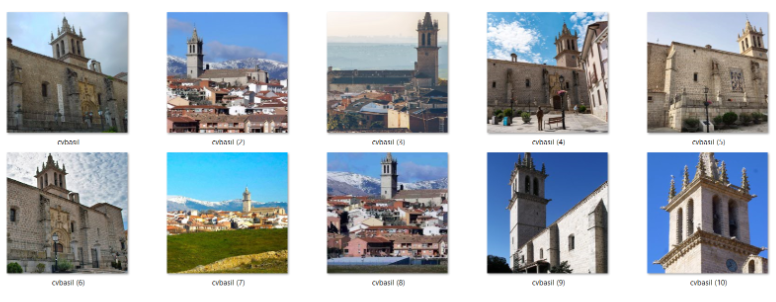
\includegraphics[width = 0.7
	\textwidth]{Imagenes/Vectorial/dataset_colmenar.png}
	\caption{Dataset seleccionado para el entrenamiento con lugares}
	\label{fig:datasetcolme}
\end{figure}


\subsection{Entrenamiento con la técnica de LORA}

Para el entrenamiento de animales, seleccionamos 10 fotografías de un perro de la raza Shiba Inu bajo diferentes perspectivas, escenarios y mostrando distintas expresiones para comprobar si la inteligencia artificial permitía entrenar con animales. Sin embargo, a la luz de los resultados vistos en personas y lugares quisimos comprobar la técnica de LORA que presenta Stable Diffusion. Las siglas LORA hacen referencia a \textit{Low-Rank Adaptation of Large Language Models}, del inglés. Esta técnica favorece un equilibrio entre el tamaño del archivo y la eficiencia del propio entrenamiento que ha presentado imágenes de gran calidad en un tiempo excepcional. 

En la figura \ref{fig:datasethachi} se pueden ver más en detalle las imágenes seleccionadas para las pruebas con LORA en animales.

\begin{figure}[h]
	\centering
	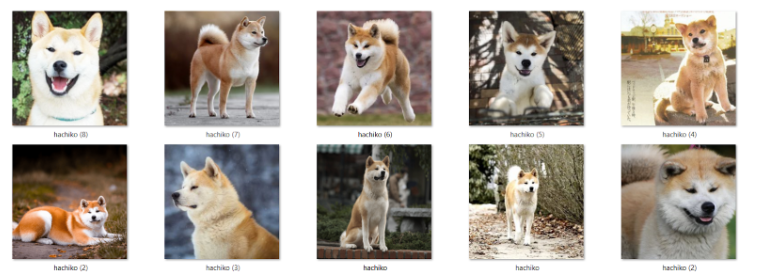
\includegraphics[width = 1
	\textwidth]{Imagenes/Vectorial/dataset_hachiko.png}
	\caption{Dataset seleccionado para el entrenamiento con animales}
	\label{fig:datasethachi}
\end{figure}

Como se puede apreciar en la figura anterior, se hizo hincapié en la diversidad de las imágenes, para aportar un mayor valor al entrenamiento, de modo que se tuviese una visión completa del elemento a entrenar.

Respecto al modo de ejecución, el hecho de cambiar a LORA no supuso grandes cambios a la hora de entrenar el elemento deseado debido a que la selección de imágenes es exactamente igual. Donde realmente cambia el entrenamiento es en el cuaderno utilizado en Google Colab, este es diferente y por lo tanto, la forma de ejecución y los pasos a seguir también lo son. 

Es de vital importancia saber cuáles son los parámetros que se deben ajustar para poder desarrollar el modelo de manera correcta y entender cada uno de ellos, dado que pueden resultar un poco más complejos en comparación con la técnica del cuaderno de Fast-Dreambooth.\\

El cuaderno de LORA de Google Colab, a diferencia del de Fast-Dreambooth, contiene una única celda de código con varios parámetros a ajustar y que  está ordenada en varias secciones. La primera sección es "Setup", lo que se puede traducir como la configuración o preparación, en ella se exige indicar el nombre del proyecto, la estructura de carpetas y por último, se debe especificar el modelo a entrenar entre tres opciones dadas (Anime, AnyLora y Stable Diffusion), y como se ha explicado anteriormente, hemos elegido el Stable Diffusion 1.5, al ser el que sirve de base para todos los entrenamientos escogidos. No obstante, esta técnica de entrenamiento tiene la peculiar característica de que se puede utilizar de base cualquier checkpoint desarrollado previamente, por lo que en caso de realizar un entrenamiento sobre personas, existe la posibilidad de elegir un modelo de base especializado en retratos. Esto garantiza que, seleccionando unas fotografías adecuadas y ajustando de manera correcta cada parámetro, los resultados sean bastante buenos.\\

La siguiente sección se llama "Processing", el parámetro más destacable en este apartado es la resolución de la imagen, a elegir entre 512, 640, 768, 896 y 1024. La elección dependerá del tamaño mínimo que tenga la imagen más pequeña de nuestro dataset.  En particular, y habiendo realizado múltiples entrenamientos con LoRA, cabe destacar que lo más recomendable es dejar la resolución de la imagen en 512 píxeles, es decir, tal y como aparece. Esto es porque aumenta considerablemente el tiempo de entrenamiento cuanto más alta es la resolución. Si se diera el caso de que esto provocase un aumento significativo en la calidad de las imágenes generadas, podría ser muy beneficioso. No obstante, entre una resolución de 512 y 1024 no se aprecia un gran salto de calidad, pero sí de tiempo, ya que aumenta desde los 20 minutos hasta más de una hora de tiempo de entrenamiento. Los demás parámetros son tags o etiquetas sobre la simetría y calidad de las imágenes. \\

Terminada esta, empieza la próxima sección ``Steps".
En cuanto a los steps de entrenamiento, en LoRA se deben indicar de un modo diferente, y aquí sí que presenta una gran ventaja respecto al modelo de Dreambooth. En este otro modelo, se indicaba un número concreto de pasos y como resultado, obteníamos un archivo en formato ckpt, de dos gigas de tamaño. Sin embargo, en LoRA se puede indicar un número de archivos que se deseen obtener. La peculiaridad de esto, es que cada número de pasos que se indique, se genera un resultado. De esta manera, en un mismo entrenamiento, se puede comprobar cuál es el número de pasos que genera la mejor fotografía. Este número de resultados se denomina \textit{epochs}, y en num repeats, se puede indicar el número de pasos que se entrenarán en cada \textit{epoch}. \\

\begin{figure}[h]
	\centering
	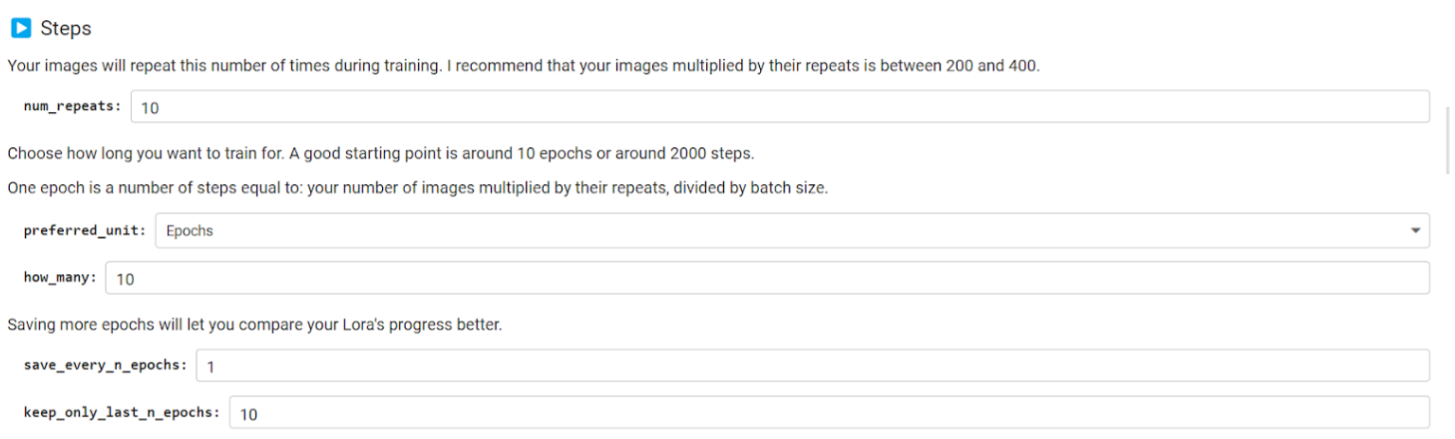
\includegraphics[width = 1.2
	\textwidth]{Imagenes/Vectorial/lora.png}
	\caption{Parámetros relevantes del entrenamiento con LoRA}
	\label{fig:lora}
\end{figure}

Por ejemplo, si se indica en este valor un 10, se obtendrá como resultado diez archivos en formato \textit{safetensor}. Estos archivos tienen un tamaño de alrededor de 18 MB, un tamaño mucho menor que un \textit{checkpoint}, de 2 GB. La diferencia reside en que el \textit{checkpoint} es un modelo nuevo a partir de uno pre entrenado, y el \textit{safetensor}, únicamente contiene el elemento que se ha entrenado, y para su ejecución necesita ir acompañado de su modelo de origen, en este caso el Stable Diffusion 1.5, lo que se ve reflejado en la siguiente imagen. De ahí nace la significativa diferencia de tamaño, por lo que, en cuanto a espacio de almacenamiento, es mejor la técnica de entrenamiento de LoRa. \\


Las secciones siguientes ``Learning'' de aprendizaje y ``Structure'' de estructura se refieren a variables que no se deben modificar del entrenamiento a cómo están preestablecidas, y por lo tanto, no hemos incidido en ellas.

Finalmente, la sección ``Ready'' nos indica que está ya todo listo para poder empezar el entrenamiento con LORA. \\

Ahora podemos decir que hemos logrado entrenar un modelo de generación de imágenes incluyendo fotografías propias, y eso es algo que puede ser realmente útil para nuestros siguientes propósitos. Esto es porque podemos lograr que cualquier persona pueda incorporar las imágenes que considere oportunas para servir de apoyo al paciente. Lo cual consideramos un éxito en el desarrollo de nuestro trabajo. 


\section{Interfaz de Stable Diffusion}

\subsection{Requisitos de instalación}

Respecto a los requisitos que debe cumplir un equipo para que pueda funcionar la aplicación NMKD Stable Diffusion GUI, es fundamental que tenga un mínimo de 8 GB de memoria RAM, siendo lo más recomendable que sea de 16 GB. También es muy importante el almacenamiento, donde además de tener un mínimo de 10 GB de espacio disponible, es conveniente que haya 5 GB extras, debido a que se van a guardar multitud de archivos temporales a medida que se utiliza la aplicación. Adicionalmente, para nuestro caso, que hemos utilizado la aplicación para comparar diferentes modelos, es necesario conocer que cada uno de ellos tiene un tamaño de alrededor de 5 GB, y los modelos entrenados derivados de Stable Diffusion ocupan 2 GB de almacenamiento cada uno. Por lo tanto, el espacio es algo que hay que tener muy en cuenta previamente a la instalación de este programa, ya que puede comprometer seriamente el funcionamiento del equipo. \\

La característica principal que debe cumplir un equipo y sin la cual no sería válido para utilizar la aplicación es el hecho de tener una tarjeta gráfica. Además, no sirve cualquier GPU, dado que el mínimo de memoria VRAM que debe tener el equipo es 4 GB, siendo la tarjeta de Nvidia. Más allá de que este sea el mínimo para que la aplicación funcione, a medida de que la tarjeta gráfica sea de mayor calidad y espacio, el rendimiento mejora exponencialmente. Para contextualizar, la tarjeta gráfica de nuestro equipo, una Nvidia GeForce GTX 1050, con una memoria de vídeo dedicada de 3072 MB y una memoria virtual disponible de 8 GB, tarda alrededor de varios minutos en generar una fotografía con cierta calidad. Mientras tanto, tarjetas gráficas como la RTX 4090, genera las imágenes en 1 segundo, lo cual es bastante significativo. No obstante, esta tarjeta tiene un precio en el mercado de alrededor de 2000 euros, por lo que en nuestro nivel, mejorar el rendimiento es algo que se antoja complicado, y que la duración que va a tener nuestro proceso de generación de imágenes será siempre de varios minutos.\\


\subsection{Funcionamiento y detalles de la interfaz}

 Respecto al funcionamiento de SDGUI, esta plataforma tiene una interfaz muy sencilla para el usuario, a pesar de que hay que tener conocimientos previos acerca de ciertos parámetros para poder llevar a cabo la generación de de imágenes, además de realizar múltiples pruebas para saber qué función cumple cada elemento. La aplicación se presenta tal y como aparece en la siguiente imagen, y permite generar imágenes con modelos de Stable Diffusion, con modelos obtenidos de Hugging Face, con modelos entrenados y con LoRA. Esto ofrece una gran ventaja para nuestro trabajo, ya que ha sido el programa que nos ha permitido probar qué modelo era el más adecuado para nuestro estudio, y posteriormente testar los entrenamientos realizados. Ha sido fundamental, porque han sido miles de pruebas, ajustando todos los parámetros de múltiples maneras diferentes, y sin esta aplicación, avanzar y obtener resultados habría sido realmente complicado. Respecto a la estructura del programa, cuenta con una parte derecha de la pantalla, donde aparecen las imágenes generadas en un gran recuadro, se puede acceder a un historial de descripciones introducidas y se puede acceder a una carpeta que incluye todas las imágenes que han sido generadas por esta aplicación. Además, en la parte superior, se puede acceder a ajustes, donde es posible instalar nuevas versiones del programa u obtener nuevos modelos que poder utilizar para la generación de imágenes. \\
 
 
 \begin{figure}[h]
 	\centering
 	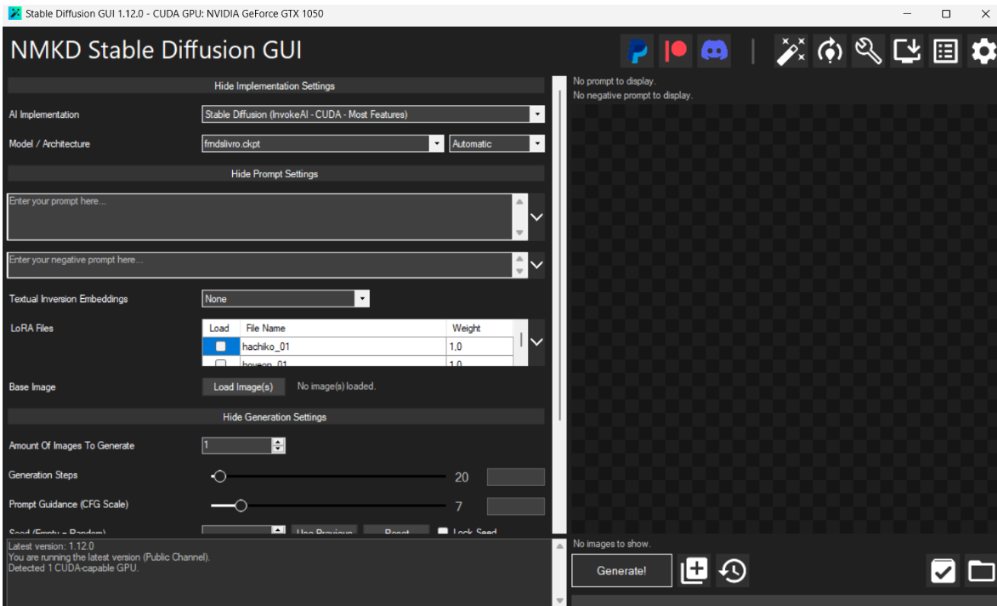
\includegraphics[width = 1
 	\textwidth]{Imagenes/Vectorial/nmkdsdgui.png}
 	\caption{Aplicación SDGUI, utilizada para probar todos los modelos generadores de imágenes }
 	\label{fig:nmkdsdgui}
 \end{figure}
 
 En la parte izquierda de la pantalla, podemos encontrar los parámetros realmente importantes que condicionan la manera en la que se creará la siguiente fotografía. En primer lugar, el tipo de inteligencia artificial utilizada. Esto es realmente relevante porque hace una distinción de cuatro tipos de IA generativa: dos son versiones estándar de Stable Diffusion (una para los sistemas que utilicen CUDA o Nvidia, y otra para los que utilicen AMD como tarjeta gráfica), la tercera es la versión XL de Stable Diffusion, que como recordatorio, requiere una tarjeta gráfica muy superior a la que dispone nuestro equipo, y por último, un modelo imagen a imagen. Resulta muy relevante hablar sobre esta IA, dado que a partir de una imagen de archivo, y una descripción, se puede generar una nueva imagen adaptada a esta petición. A pesar de que nuestro objeto de estudio abarca la inteligencia artificial generativa de imágenes a partir de texto, hemos realizado pruebas sobre el tipo de resultado obtenido, pero la calidad de la imagen de este modelo en concreto, resulta inferior a la que nos han otorgado modelos de texto a imagen. Centrándonos en el modelo básico de Stable Diffusion, en el apartado de \textit{model} / \textit{architecture}, se debe incluir el modelo, que puede ser uno pre entrenado o uno personalizado en formato \textit{checkpoint}. En este segundo, cabe destacar que tarda medio minuto más en generar la fotografía debido a la carga, pero no afecta de ninguna manera a la calidad de la imagen. \\
 
 A continuación, se debe indicar la descripción, que se divide en dos partes en este caso. La primera es el \textit{prompt}, que guía a la inteligencia artificial para que incluya los elementos que se deseen. Un apunte relevante es que si se quiere hacer referencia a un elemento entrenado, se debe mencionar el nombre exacto del ítem para que se pueda realizar la generación de manera correcta. En segundo lugar, existe un \textit{negative prompt}, donde se deben indicar aquellos elementos que, a petición del usuario, se desee que no se vean reflejados en la creación de la fotografía. Cuando se desee testar un entrenamiento de LoRA, se debe hacer click en el archivo deseado, e introducir ese nombre en el \textit{prompt}. Por último, se deben ajustar unos parámetros explicados con anterioridad, como son los \textit{steps} o pasos de generación, la escala CFG y la \textit{seed}. Una vez conocidos estos pasos a seguir y cumplidos los requisitos mencionados, cualquier usuario debería tener la capacidad de generar imágenes mediante inteligencia artificial con este programa.\\

\section{Resultados de generación de imágenes}

Visto el funcionamiento de la aplicación, vamos a analizar los resultados obtenidos en comparación con los \textit{prompts} especificados y bajo las posibles diferentes técnicas y parámetros que se han contemplado. 


\subsection{Resultados con personas}
Una buena manera de mostrar el mejor resultado posible de una generación de imágenes personalizadas es estudiar cuál es el método que genera mejores fotografías. Para ello, hemos realizado un análisis comparativo de resultados con diferentes pasos de entrenamiento.

El objetivo es comprobar cuál es el número de pasos del entrenamiento mediante Dreambooth que genera las imágenes con mayor calidad y precisión posible. Para ello, hemos realizado cuatro entrenamientos del mismo elemento, con el mismo \textit{dataset} de 10 fotografías, pero con un número de pasos diferente. Este número ha sido de 1600, 2000, 2400 y 3000 \textit{steps}. El tiempo de generación aproximada es de 1,38 iteraciones por segundo, lo cual conlleva una duración total de entrenamiento de 19, 24, 29 y 35 minutos aproximadamente, y es algo a tener en cuenta para seleccionar un modelo u otro.\\

Para poder llegar a resultados concluyentes, se han de fijar todas las variables de la generación de imágenes en la aplicación SDGUI. Estas variables son la descripción de la fotografía, los pasos de generación, la escala CFG y la semilla de aleatoriedad. De esta manera, se tiene la capacidad de realizar una comparación precisa y de elegir el número más adecuado de pasos de entrenamiento. En este caso, dada nuestra experiencia al generar imágenes con Stable Diffusion, establecimos el número de pasos en 20 y la escala CFG en 7. Respecto a la semilla de aleatoriedad, tras la primera fotografía generada se fijaría para el resto, para que permanezca constante en nuestro análisis.\\

Hemos optado por utilizar varios tipos de fotografía diferente para poder ampliar la calidad de la conclusión. La primera descripción de imagen trataba de generar un retrato de la persona lo más detallado posible, de manera que se pudiera comparar con qué pasos la capacidad de identificar al elemento entrenado era mayor. Con el segundo \textit{prompt}, se pretendía analizar la generación de las imágenes de la persona haciendo una acción determinada. En este caso, se optó por la lectura de un libro. De este modo, se podría afirmar cuál de los modelos tendría la capacidad de generar fotografías personalizadas de múltiples elementos, lo cual es algo bastante relevante para nuestro trabajo. Por tanto, en la siguiente tabla se refleja la imagen generada con cada número de pasos de entrenamiento, con las dos descripciones mencionadas.\\

Figura X:\\

Tras generar todas las fotografías, en primer lugar, se aprecia falta de entrenamiento en las dos imágenes con 1600 \textit{steps}, debido a que no se identifica bien a la persona, ni en el retrato, ni en la imagen con el libro. En la primera fotografía se puede observar una gran calidad, con mucho detalle y un ligero parecido con la persona entrenada, pero no es el nivel de similaridad que estamos buscando. En la imagen con el libro, la persona generada no se puede identificar con la real, y, además de eso, se aprecia deformidad en las manos, por lo que la fotografía generada no tiene el nivel de calidad deseado. \\

En segundo lugar, al incrementar los \textit{steps} de entrenamiento a 2000, se puede apreciar una clara mejoría. En el retrato, existe un gran parecido con la imagen generada con 1600 pasos, pero se aprecia como la forma de la cara se asemeja más a la persona real. Respecto a la fotografía con el libro, en esta ocasión se han solucionado los errores de deformidad, y se ha generado a una persona de la edad correspondiente, aunque no se puede identificar a la persona real.\\

Con 2400 pasos de entrenamiento, se puede decir que los resultados muestran calidad. En la primera fotografía, se puede identificar un gran parecido con la persona real. La imagen muestra un gran detalle y una definición muy buena, por lo que mejora en gran medida a los números de pasos menores. En la segunda fotografía, existe cierto parecido con la persona, pero se puede mejorar, debido a que falta detalle y definición y se muestra a alguien mucho más joven. A pesar de esto, sí que la forma de la cabeza y de la cara parecen ser correctas, por lo que lo único que faltaría para que la generación fuera adecuada es la edad, lo cual se podría arreglar con una descripción más precisa.\\

Al incrementar los \textit{steps} a 3000, se puede apreciar sobreentrenamiento, debido a que en ambas imágenes se ha perdido el parecido con la persona real y se puede percibir algo de deformidad, sobre todo en la segunda fotografía. Respecto al retrato, ha variado la forma y el color de los ojos, y han aparecido más marcas que empeoran la calidad. En la imagen con el libro, se ha generado a una persona aún más joven que con 2400 pasos, y ha cambiado por completo la forma de la cara, por lo que la similitud con la persona real se ha desvanecido por completo. Además, si se amplía en detalle se puede apreciar deformidad en los ojos, por lo que se hace evidente el sobreentrenamiento. \\

En conclusión, podemos decir que el entrenamiento que ha producido mejores resultados es el de 2400 pasos, que con menos se aprecia falta de entrenamiento y que con más \textit{steps} se percibe sobreentrenamiento y no se permite identificar a la persona real. En este estudio también se ha podido aprender que el prompt ha de ser lo más preciso posible para poder obtener imágenes de gran calidad, sobre todo cuando se trata de incluir más elementos. En este caso, la escala CFG debería ser mayor, para dar algo menos de libertad al modelo y que se centre más en lo que se pide en la descripción.


\begin{figure}[!htb]
	\centering
	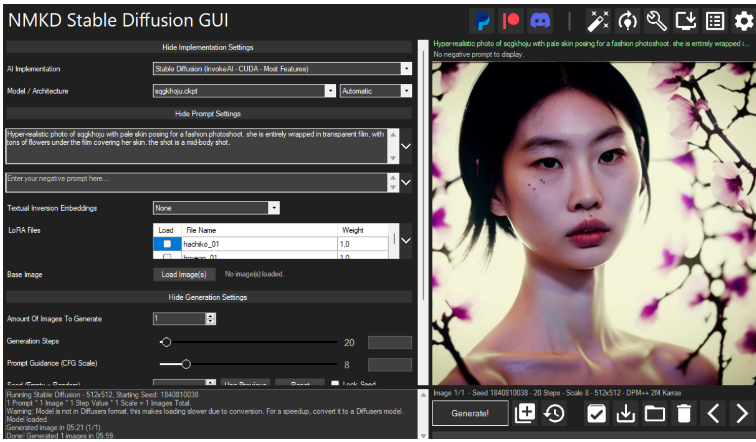
\includegraphics[width = 1
	\textwidth]{Imagenes/Vectorial/hoyeon1.png}
	\caption{Resultados de entrenamiento de una persona con Dreambooth}
	\label{fig:hoyeonsd}
\end{figure}

que tallll\\

\begin{figure}[!htb]
	\centering
	
\includegraphics[width = 1
	\textwidth]{Imagenes/Vectorial/hoyeon_results.png}
	\caption{Resultados de entrenamiento de una persona con diferentes estilos}
	\label{fig:imagshoyeon}
\end{figure}

\subsection{Resultados con lugares}

Con diferentes estilos:\\

\begin{figure}[!htb]
	\centering
	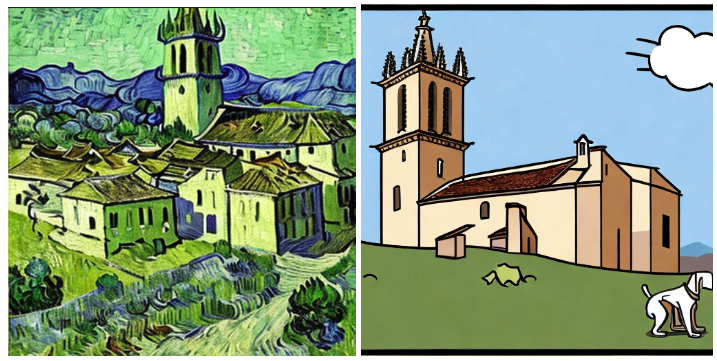
\includegraphics[width = 1
	\textwidth]{Imagenes/Vectorial/colmenar_styles.png}
	\caption{Resultados de imagenes del lugar entrenado al estilo Van Gogh y viñeta}
	\label{fig:colmestyles}
\end{figure}


Añadiendo otros elementos:\\


\begin{figure}[!htb]
	\centering
	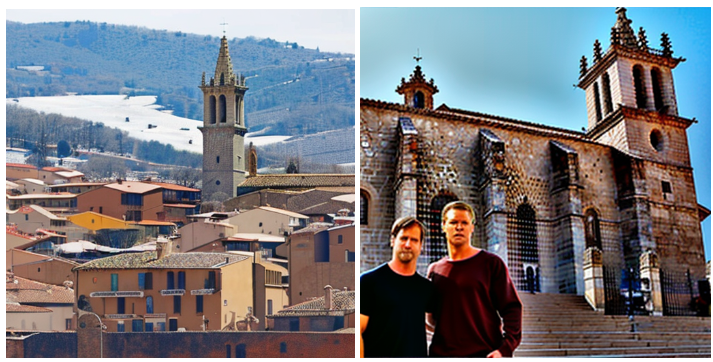
\includegraphics[width = 1
	\textwidth]{Imagenes/Vectorial/colmenar_elements.png}
	\caption{Resultados de imágenes del lugar en invierno y con una persona}
	\label{fig:elementscolme}
\end{figure}

\subsection{Resultados con animales}
hellloouuuuu\\

\begin{figure}[!htb]
	\centering
	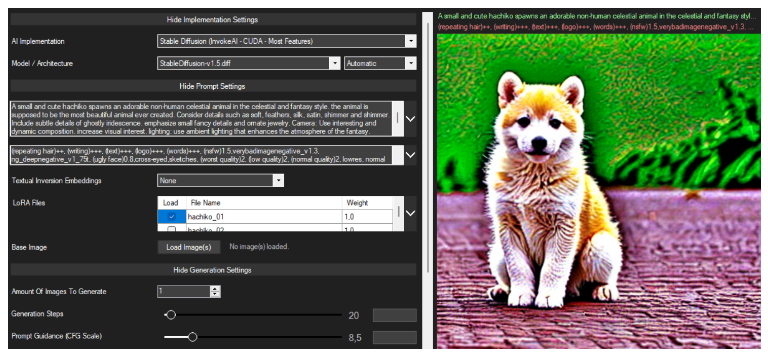
\includegraphics[width = 1
	\textwidth]{Imagenes/Vectorial/hachiko_detallada.png}
	\caption{Imagen generada con el modelo Stable Diffusion 1.5, Lora Hachiko}
	\label{fig:detallehachi}
\end{figure}

heyyyyy\\

\begin{figure}[!htb]
	\centering
	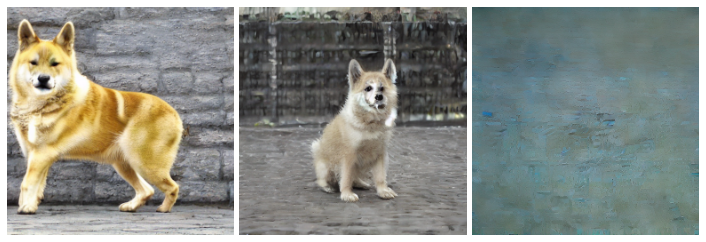
\includegraphics[width = 1
	\textwidth]{Imagenes/Vectorial/comparacion_hachiko.png}
	\caption{Mismo prompt con 1000, 2000 y 10.000 pasos de entrenamiento}
	\label{fig:comphachi}
\end{figure}

\subsection{Resultados con múltiples capas de entrenamiento}

Una parte muy importante de nuestro trabajo es generar imágenes que puedan contener diferentes elementos de manera simultánea, puesto que consideramos que para crear un libro de vida de calidad, se deberían incluir fotografías de una persona en un determinado lugar, o que combinen varias personas diferentes. Durante la mayor parte del tiempo en la que realizamos este proyecto, teníamos la idea de que esto no sería posible, porque siempre que realizábamos pruebas, obteníamos resultados en los que se deformaban los elementos, o simplemente solo incluía uno de los dos elementos, o ninguno de los dos. 

A pesar de esto, decidimos resistirnos a aceptar que no podía ser posible una generación de imágenes en la que se combinasen varios elementos. Como hemos afirmado en apartados anteriores, nuestro modelo de entrenamiento Dreambooth permite realizar un entrenamiento sobre otro previo, por lo que decidimos hacer la prueba y añadir una capa. Para el entrenamiento, utilizamos como base el archivo sqgkhoju.ckpt, el cual entrenó a la actriz Jung Hoyeon, y se entrenó con el salón de la serie \textit{Friends}. Como en el resto de pruebas con las que obtuvimos un resultado satisfactorio, incluimos un conjunto de 10 imágenes y realizamos el entrenamiento con 2400 pasos.\\

\begin{figure}[!htb]
	\centering
	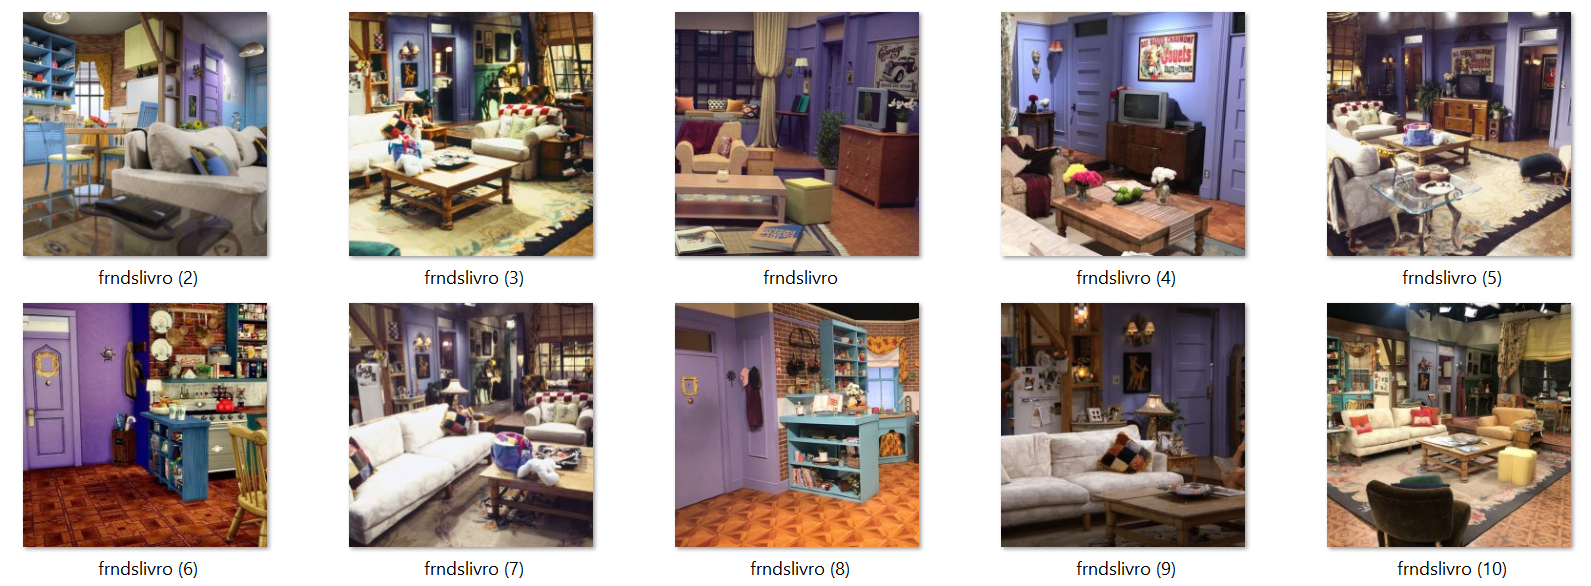
\includegraphics[width = 1
	\textwidth]{Imagenes/Vectorial/dataset_frdslivro.png}
	\caption{Dataset del entrenamiento con el salón de Friends (frndslivro)}
	\label{fig:dataset_frdslivro}
\end{figure}


Una vez realizado el entrenamiento, en primer lugar, se comprobó que se podían generar buenas fotografías que incluyesen únicamente el salón, antes de crear imágenes con ambos elementos.\\

\begin{figure}[!htb]
	\centering
	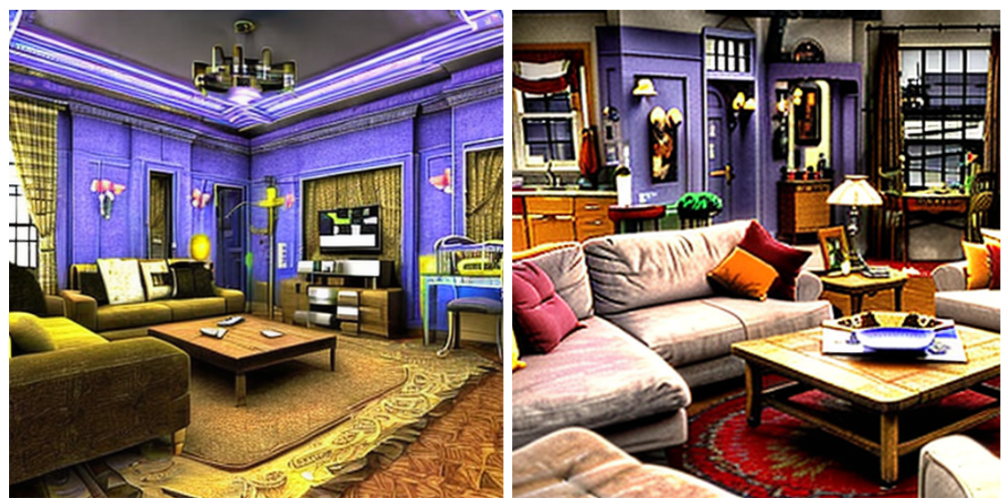
\includegraphics[width = 1
	\textwidth]{Imagenes/Vectorial/resultadosfrndslivro.png}
	\caption{Resultados de la generación de imágenes con el modelo ``frndslivro''}
	\label{fig:resultsfrnds}
\end{figure}

Como se puede apreciar, las imágenes generadas son de calidad, están creadas con 20 pasos de generación, 8 de \textit{CFG scale} y con diferentes estilos. Viendo que el modelo genera las fotografías de manera exitosa, es el momento de crear imágenes de la persona en el salón. Siguiendo la tendencia de 20 pasos y 8 de CFG, se producían errores en la generación, creándose imágenes en las que aparecía la persona duplicada y no aparecía el lugar. Ateniéndonos a la definición de \textit{CFG scale}, subimos este valor, de 8 a 14, para que la inteligencia artificial se guiase en mayor medida por el \textit{prompt}. Con solo subir este valor no fue suficiente, pues generaba fotografías en las que la persona aparecía entre 3 y 4 veces. Por tanto, también decidimos aumentar los pasos de generación, de manera sucesiva hasta que la generación produjera un resultado satisfactorio. La combinación perfecta fue de 40 pasos y 14,5 de \textit{CFG scale}. Con un número menor de \textit{steps}, la imagen aparecía con múltiples personas, y con un número mayor, no generaba ninguna persona. La descripción de la imagen era la siguiente: a ``sqgkhoju in the frndslivro, hd, high quality''.\\

\begin{figure}[!htb]
	\centering
	
\includegraphics[width = 1
	\textwidth]{Imagenes/Vectorial/resultadoshojuyfrnds.png}
	\caption{Mismo prompt con 20, 40 y 50 steps al mezclar dos elementos: persona y lugar}
	\label{fig:comphachi}
\end{figure}


\subsection{Logros y fallos en resultados}

A lo largo de la variedad de entrenamientos realizados hemos hecho pruebas exhaustivas sobre la generación de las imágenes en comparación con los \textit{prompts} especificados y hemos sacado en claro que hay 3 aspectos fundamentales que hay que tener en cuenta para la generación óptima de estas: el número de pasos realizados en el entrenamiento, en el número de pasos para la generación de la foto y la escala CFG. 

En los tres aspectos, hemos identificado dos posibles situaciones que se pueden dar y que presentan fallos en cuanto a la calidad de los resultados: exceso y falta de pasos en el entrenamiento. 


- Peligros con el sobreentrenamiento: Se produce cuando el modelo no se puede generalizar y se ajusta demasiado al conjunto de datos entrenados. Se debe principalmente a que el tamaño de los datos es demasiado pequeño y no contiene suficientes muestras de datos para poder representar con precisión la totalidad de datos de entrada posibles. Otra razón es que el modelo se entrena durante demasiado tiempo en un solo conjunto de datos de muestra. En nuestro modelo, encontramos sobreentrenamiento cuando elegimos un número de \textit{steps} muy elevado para un número de fotografías que no es lo suficientemente alto. Una manera de detectar que nuestro modelo está sobreentrenado es cuando no genera bien la cara de la persona, y se aprecian fallos en determinadas facciones, como en los ojos y la boca, en los cuales se aprecia deformidad.\\

- Falta de pasos en el entrenamiento: En este caso, se produce cuando el modelo de datos no tiene la capacidad de capturar de forma precisa la relación entre las variables de entrada y de salida, de manera que existe un elevado índice de errores en el conjunto de datos de entrenamiento y en los datos no vistos. Se debe a que el modelo es demasiado simple, porque el tamaño de los datos es demasiado pequeño, o bien porque se necesita más tiempo de entrenamiento. En este caso, cuando generamos las imágenes, se evidencia que el modelo aún no ha aprendido lo suficiente acerca del elemento o \textit{token} del que se ha realizado el entrenamiento, pues el resultado de la generación refleja una persona que no muestra ningún parecido con la realidad.\\


En cuanto a mezcla de personas: Para ampliar los horizontes de nuestro entrenamiento, hemos entrenado a una persona, asociando un \textit{token} a ella para su identificación, sobre un modelo que previamente ya había sido entrenado con una persona y su \textit{token} asociado, para comprobar si efectivamente se podía generar en una sola imagen una representación de las dos personas entrenadas, una junto a la otra. Es aquí donde se ha detectado una peculiaridad, ya que, a pesar de que un modelo genere buenos resultados de cada una de las dos personas, en el mismo momento que se solicita en un determinado \textit{prompt} o descripción que se vean reflejados una o varias personas entrenadas en la misma fotografía, ningún modelo de los que se haya probado, ha generado buenos resultados de esta manera. Lo que finalmente se aprecia en la imagen generada, es que aparecen dos personas pero sus rostros son una mezcla de las características faciales y fisiológicas de ambas, produciéndose una deformidad en muchos de los casos y que los rostros aparezcan prácticamente duplicados.


\begin{figure}[h]
	\centering
	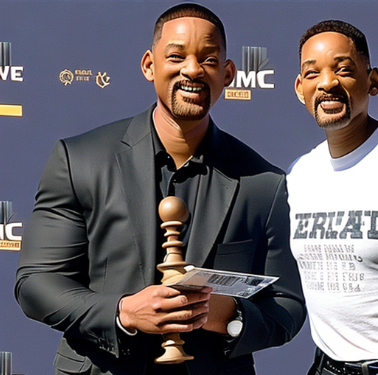
\includegraphics[width = 0.5
	\textwidth]{Imagenes/Vectorial/duplicidad_will.png}
		\caption{Duplicidad de elementos}
	\label{fig:willpor2}
\end{figure}

\subsection{Soluciones: Técnica \textit{Inpainting}}

Debido a la importancia que consideramos que tiene en el desarrollo de unas adecuadas historias de vida la mezcla de elementos personales con la propia persona, consideramos métodos para arreglar la poca certeza que nos otorga el modelo de Stable Diffusion con múltiples capas de entrenamiento, ya que a la luz de los resultados, el modelo es, por el momento, inválido en este aspecto. \\

Por ello, decidimos profundizar en las opciones que ofrece la interfaz de Stable Diffusion y dimos con la opción img2img, es decir, imagen a imagen. Esto es, como su nombre indica, un método en el que la entrada, en vez de ser texto como lo venía siendo hasta ahora, es una propia imagen. Sin embargo, el \textit{prompt} sigue siendo un elemento fundamental que sigue formando parte del modelo, ya que de esta manera, se le especifica a la Inteligencia Artificial lo que se desea en la imagen futura y el modelo se encargará de crearlo, teniendo en cuenta la estructura y objetos ya dispuestos en la imagen original. 

Incluso, el propio modelo de Stable Diffusion con el método de img2img tiene sus propias técnicas, de las cuales, una particularmente llamó nuestra atención: la técnica \textit{Inpainting}. 

Entre los problemas que se encontraban en el contenido final de las imágenes pedidas bajo un \textit{prompt} que integraba dos elementos entrenados, podíamos distinguir 3 casos principales: contenido aleatorio no especificado, falta completa de uno de los dos elementos o un elemento y el concepto del segundo elemento sin llegar a ser el propio. 

Por tanto, podemos llegar a afirmar que el último caso es el que más se asemejaba a lo que queríamos llegar a conseguir. Por ejemplo, si en el \textit{prompt} especificábamos que apareciera el \textit{token} que se asocia a una persona entrenada junto al \textit{token} asociado a un animal entrenado, la gran mayoría de los resultados era el perro entrenado a la perfección junto a una persona que no se asemejaba de ninguna manera a la entrenada.  

Lo que nos llegó a pensar que realmente la imagen generada de por sí, no era del todo errónea, ya que tan solo necesitábamos cambiar una pequeña porción de la misma: la persona de la imagen por la entrenada por nosotros en el modelo. Y es precisamente lo que logra la técnica de \textit{inpainting}. 

Esta novedosa técnica debe su nombre a que el protagonista es un pincel virtual. Para ejecutarla, necesitamos como entrada una imagen, en nuestro caso, la imagen recién generada por el modelo que presenta una carencia. Con el pincel, dibujamos el área de la imagen que deseamos sustituir por otro elemento. Y a través del \textit{prompt}, especificamos aquello que solamente queremos que aparezca en el área trazada, en este caso, el \textit{token} que representa a la persona entrenada. 

De esta manera, la Inteligencia artificial genera lo especificado en el \textit{prompt} solamente en el área indicada sustituyéndolo por lo que había anteriormente. En este ejemplo, el área que dibujaríamos correspondería a la persona de la foto y el resultado final serían los dos elementos diferentes integrados a la perfección en una sola imagen. 

Debido a la novedad de la técnica, los parámetros que estábamos acostumbrados a cambiar, también se han ampliado para poder emplear la técnica con los mejores resultados posibles y de la manera más eficiente. 

Entre ellos, los más importantes y que se pueden ver en la figura \ref{fig:paramsinpainting} señalados, son 5, con los cuales dos ya estamos familiarizados, que son los \textit{steps} y \textit{cfg scale}. Por lo tanto, nos centraremos más en los 3 restantes. 

\begin{figure}[h]
	\centering
	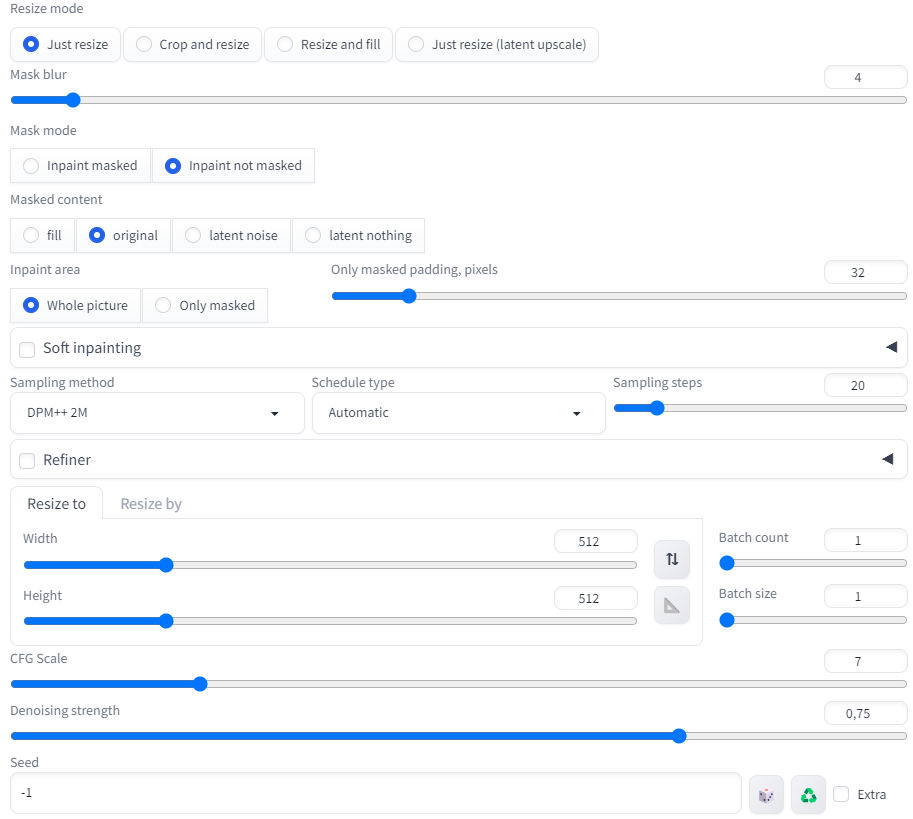
\includegraphics[width = 0.6
	\textwidth]{Imagenes/Vectorial/parametrosinpainting.png}
	\caption{Configuración de los parámetros en la técnica de inpainting}
	\label{fig:paramsinpainting}
\end{figure}

El primer parámetro es ``\textit{Mask Mode}'' y antes de continuar, es importante especificar que en \textit{Inpainting}, cuando se habla de ``\textit{mask}'' se refiere únicamente al área que hemos marcado con el pincel para su posterior modificación. Como podemos ver en la figura \ref{fig:gan}, en este parámetro se encuentran dos opciones: \textit{inpaint masked} e \textit{inpaint not masked}. A lo que se refiere es al área que se va a ver sustuida por el \textit{prompt}, ya que habrá casos en los que se quiera conservar la imagen en su totalidad a excepción de una parte y casos que por el contrario, se desearía modificar la imagen en su totalidad, a excepción de una porción, como lo puede ser en el caso de un cambio de fondo. 

El segundo parámetro es ``\textit{Masked content}'' y las opciones que presenta son un poco más extensas que en el parámetro anterior, siendo estas \textit{fill}, \textit{original}, \textit{latent noise} y \textit{latent nothing}. Lo interesante de estas opciones es el funcionamiento que lleva a cabo Stable Diffusion en la generación de contenido en el área especificada. Como ya hemos podido ver en el Capítulo 2, Stable Diffusion necesita o bien ruido o bien nuevos datos para generar una imagen, y al tener la opción a original, se trabajará a partir del contenido de la foto original, es decir, se coge de referencia la forma y colores originales para la generación. En general, se recomienda no cambiar estas opciones y siempre mantener la que está por defecto, es decir, original. 

Por último, el tercer parámetro ``Denoising Strength'' es un valor entre 0 y 1 que explica la fuerza en la que cambiará el área seleccionada en comparación la imagen original, siendo el 0 que no cambie nada y el 1 algo completamente diferente. 

Cabe destacar que la técnica de \textit{inpainting} implementada a través del método de imagen a imagen no está incorporada en la aplicación NMKD SD GUI y por ello, se han tenido que buscar alternativas para acceder a ella. En concreto, hablamos de un cuaderno de trabajo hecho en Google Colab en el que se ha importado código de GitHub de Automatic1111, una conocida interfaz gráfica destinada a usar herramientas avanzadas de Stable Diffusion. La principal ventaja que presenta este cuaderno es que permite cargar un modelo propio ya entrenado, como se puede ver en la figura \ref{fig:inpainting1} que el modelo cargado es el archivo frndslivro.ckpt visto en este mismo capítulo anteriormente. Lo cual es perfecto para el objetivo que queremos conseguir. 

\begin{figure}[h]
	\centering
	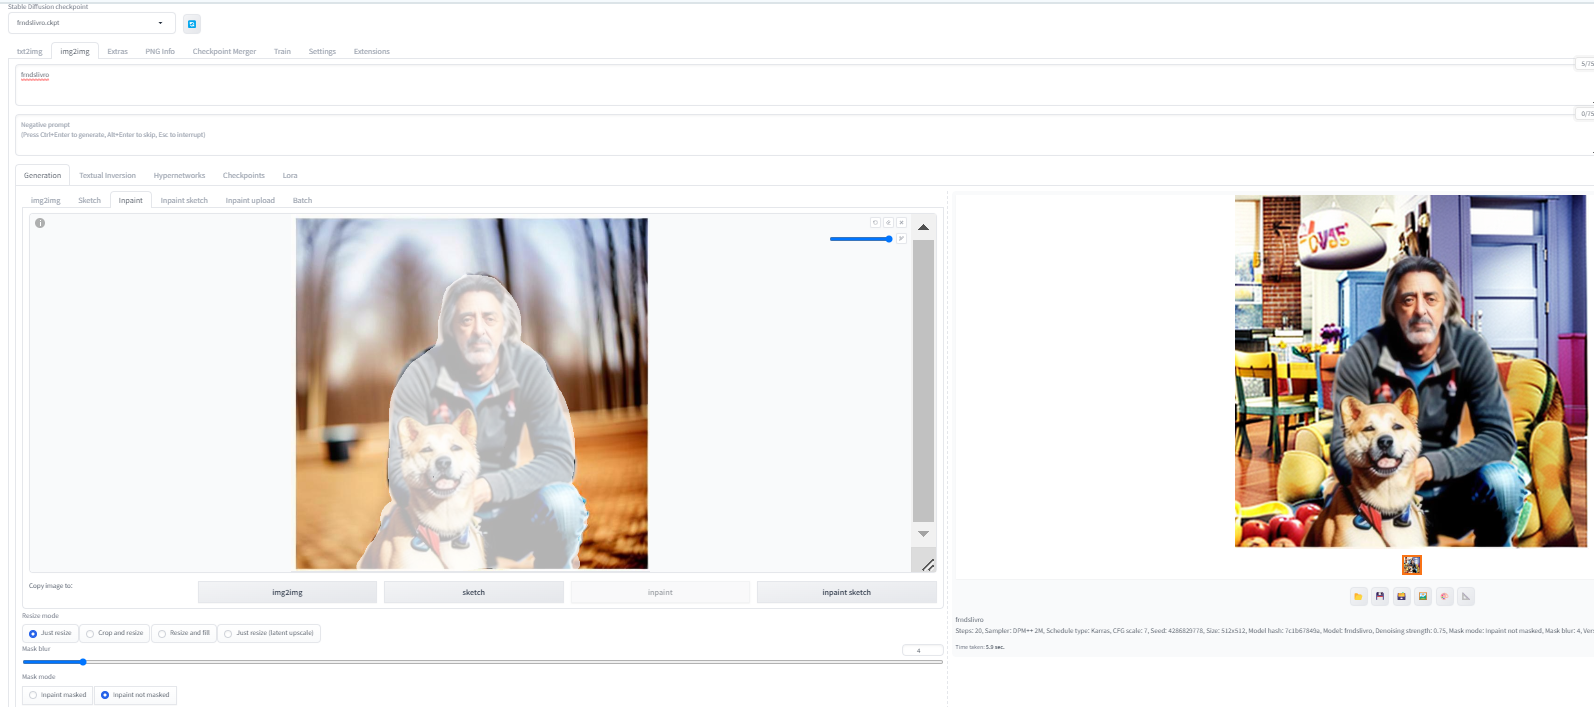
\includegraphics[width = 1
	\textwidth]{Imagenes/Vectorial/inpainting1.png}
	\caption{Ventana de la WEBUI implementada para realizar el painting}
	\label{fig:inpainting1}
\end{figure}

En la figura \ref{fig:inpainting1} se puede ver a la derecha la imagen ``original'', la cual previamente ya había sido pasada por esta técnica para poner la cara de ``80alp'' en la persona anteriormente generada. En la misma figura se puede ver el área \textit{masked} seleccionada con el pincel y el parámetro ``\textit{Mask mode}'' establecido a ``\textit{Inpaint not masked}''. Finalmente, podemos ver en el \textit{prompt} que solamente se especifica el \textit{token} ``frdslivro'' debido a que lo que se quiere conseguir es que sustituya lo que no está seleccionado por la brocha en la imagen, por el salón entrenado del modelo. El resultado puede verse en la parte derecha de la imagen, el cual podemos afirmar que es todo un éxito, al haber conseguido incorporar 3 \textit{tokens} entrenados diferentes, la persona, el animal y el lugar. 

En el siguiente ejemplo de la figura \ref{fig:fasesinpainting} podemos ver la evolución que sigue una misma imagen bajo diferentes peticiones de \textit{prompt} en la fase de \textit{inpainting}. En la primera imagen que se ve en la figura, el \textit{prompt} especificado fue ``a happy 80alp walking with his dog hachift80alp in the forest next to the mountains, day light, full hd, high quality'' y podemos ver como generó todo a la perfección excepto a la persona entrenada. En la segunda foto, se partió de la primera imagen y trazando el área del rostro de la persona, se puso como prompt ``a close up picture of 80alp face, hd''. Finalmente, para que el cuerpo de la persona generada al principio encajara con el de una persona de la edad de la foto, se seleccionó la ropa como área y finalmente el prompt fue ``old man clothes'' y el resultado final fue excepcional. 

\begin{figure}[h]
	\centering
	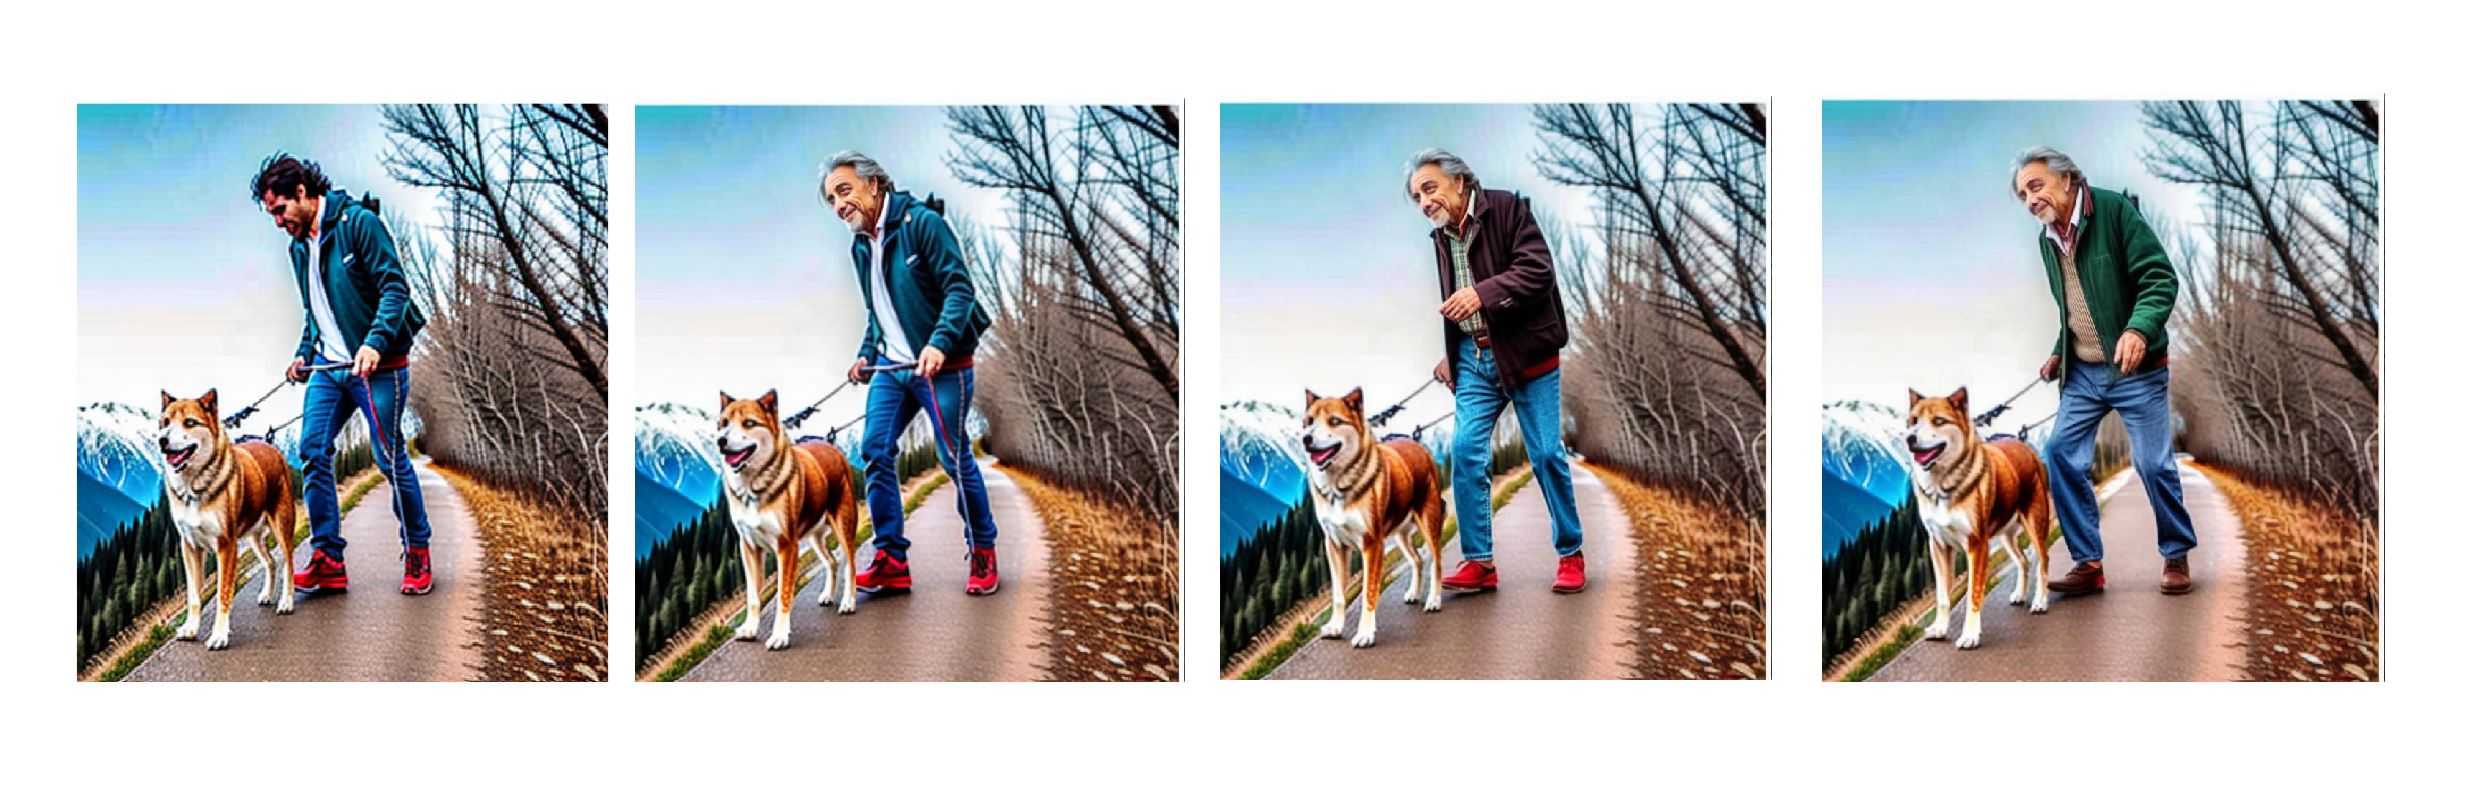
\includegraphics[width = 1.1
	\textwidth]{Imagenes/Vectorial/fasesinpainting.png}
	\caption{Evolución de una imagen con la técnica de inpainting aplicada}
	\label{fig:fasesinpainting}
\end{figure}

\section{Evolución de los modelos del proyecto}

Este apartado muestra los pasos que se han llevado a cabo durante la realización del proyecto. Resulta significativo porque el contraste de lo que se podía hacer al principio con lo que se puede hacer ahora es muy elevado, y pone en valor el trabajo realizado.

1. No se podían generar imágenes en local. No estaba instalado CUDA en el equipo, además de otras herramientas necesarias como Diffusers.

2. Generación de imágenes en local por consola en Anaconda mediante el modelo de Stable Diffusion 1.5. Resultado generado en un archivo. Ejecución lenta y de poca calidad.

3. Generación de imágenes en SDGUI. Buena interfaz que permite la ejecución de imágenes con Stable Diffusion 1.5. Mejor tiempo y calidad. Ya sabemos el modelo más óptimo para desarrollar nuestro proyecto.

4. Se descubre que se pueden utilizar más modelos provenientes de Hugging Face en SDGUI. Se utiliza el Lykon Dreamshaper, basado en LCM, que proporciona alta calidad con muchos menos pasos. No obstante, tiene la limitación de que no se puede personalizar y desarrollar.

5. Intento de generar imágenes personalizadas. Se probarán en SDGUI. Resultados aceptables con LORA. Se puede identificar al elemento entrenado, pero se puede mejorar.

6. Nuevas vías de entrenamiento de modelos. Entrenamiento de Stable Diffusion con Dreambooth. Se identifica el elemento pero se aprecia deformidad.

7. A base de prueba y error, se llega a la conclusión de que el mejor rendimiento se consigue con 2400 pasos de entrenamiento y un dataset de 10 imágenes. Buena calidad en las personas entrenadas, sin deformidad.

8. Se consiguen buenos resultados también en lugares y animales, además de en personas. Se llega a la conclusión de que se puede entrenar cualquier elemento.

9. Se quiere crear una aplicación que utilice esta IA generativa. Al principio se llega a una app con una interfaz poco visual, pero que genera buenas fotografías con el modelo Stable Diffusion 1.5.

10. Versión mejorada de la aplicación, con un backend en Python y un frontend en HTML. Buena interfaz y buenos resultados con modelos pre entrenados, pero no con modelos personalizados.

11. La aplicación ya puede utilizar cualquier modelo entrenado por nosotros mismos. Buenos resultados, con calidad y tiempo comparables a SDGUI.

12. Creación de un libro de vida para la aplicación. Sirve de conexión entre la IA generativa de imágenes desarrollada por nosotros y la creación de historias narrativas con apoyo visual para la terapia de reminiscencia.



%\include{Capitulos/Capitulo4}
%\include{Capitulos/Capitulo5}
\chapter{Conclusiones y Trabajo Futuro}
\label{cap:conclusiones}

\section{Conclusiones}

En primer lugar, podemos afirmar que, mediante la ayuda de la inteligencia artificial, se puede brindar un material fotográfico personalizado que sirva para colaborar con terapias ocupacionales, de manera que un paciente tenga la posibilidad de evocar momentos significativos, que de otra manera no tendría la capacidad de visualizar.\\

Con respecto a la generación de imágenes, se ha conseguido el objetivo de entrenar un modelo de inteligencia artificial de convertir texto a imagen, incluyendo a la persona que se considere. Este hecho significa que, en una terapia de reminiscencia, si se nos otorga un número considerable de imágenes en las que aparezca una persona concreta (a partir de diez), se puede trabajar en base a un modelo entrenado que reconozca a esa persona, y generar a partir de él las imágenes deseadas.\\

Adicionalmente, el modelo que se ha obtenido, puede servir de base para realizar un nuevo entrenamiento, lo cuál encaja a la perfección con nuestros objetivos, puesto que para un determinado paciente, podemos desarrollar un gran modelo que incluya el número de personas que se desee. No obstante, Stable Diffusion y sus modelos derivados, tienen una limitación, dado que una misma imagen es difícil de generar con múltiples elementos. Hemos logrado resultados aceptables en algunas ocasiones con un número considerable de pasos, pero requiere mucha paciencia y no podemos garantizar el éxito absoluto, como sí podemos hacerlo en una generación con un elemento principal.\\

Otro aspecto importante que debemos tener en cuenta y al que hemos llegado a la conclusión después de toda la investigación, es que para hacer funcionar nuestro modelo, al igual que cualquier otro de inteligencia artificial generativa de imágenes, se necesita una gran capacidad de memoria gráfica. Con la GPU de nuestro equipo, la generación siempre va a abarcar unos minutos, y cuanta más calidad se desee, más tiempo se incrementará. Esto es un hecho que todas las personas que se presten al servicio de generar las fotografías personalizadas deben conocer.\\

Respecto al entrenamiento de los modelos, podemos concluir que el número de pasos pasos con el que se realiza correctamente es 2400 para un entrenamiento de 10 imágenes, puesto que se han realizado múltiples pruebas con más pasos, en los que se detecta sobreentrenamiento, y con menos pasos, en los que se detecta falta de entrenamiento.\\

En base a los resultados obtenidos, podemos afirmar que el entrenamiento que maximiza la calidad de las imágenes es el de Dreambooth, con una calidad superior a la conseguida con LoRA. Con este último modelo, era mucho más difícil obtener imágenes personalizadas a partir del elemento entrenado, puesto que dadas sus características, se centraba en mostrar únicamente el elemento, ignorando los complementos que se pedían en el prompt. A través de Dreambooth, las imágenes mostraban una calidad superior y sí que se veía reflejado todo lo que se pedía en la descripción de la fotografía. Con ambos modelos de entrenamiento, podemos concluir que se puede entrenar todo tipo de elementos, ya sean personas, animales o lugares, ya que con todos ellos se han obtenido resultados correctos.\\

Con respecto a la aplicación, hemos conseguido realizar un programa, mediante el cual, se puedan generar fotografías personalizadas a partir de nuestros modelos entrenados. Esto produce muy buenos resultados y, además, permite la visualización de un libro de vida basado en una historia creada por nosotros. La idea es que un usuario pueda contar con un programa con el que pueda generar imágenes personalizadas y desarrollar un libro de vida muy atractivo de manera sencilla.\\

Podemos concluir con que hemos cumplido con los objetivos que teníamos previamente al comienzo este proyecto, puesto que hemos construido un programa mediante el cual un usuario podría obtener imágenes personalizadas con una calidad razonable en un tiempo adecuado. Ha habido una evolución constante en los últimos meses en los que se pasó de no poder generar imágenes localmente, a poder generarlas con modelos entrenados, para después poder mostrar esas fotografías en una aplicación desarrollada por nosotros.\\

\section{Propuestas de mejora}

Tras la realización de este proyecto, nos gustaría que personas encargadas de asistir a pacientes con pérdida de memoria, pudiesen realizar una investigación partiendo de nuestro modelo, con el objetivo de estudiar psicológicamente en qué medida se está favoreciendo la reducción del estrés, se está potenciando la capacidad cognitiva del paciente y se está logrando la satisfacción de las personas. Este es el mayor objetivo que tenemos con esta inteligencia artificial, lograr el bienestar personal, y el alcance de este trabajo no nos permite comprobar si realmente hemos obtenido grandes resultados en el aspecto social.\\

Adicionalmente, sería conveniente que si este proyecto fuese utilizado por los terapeutas, deberían tener un equipo con una gran tarjeta gráfica, para que se invirtiera así el menor tiempo posible en la generación de las imágenes. Tras haber utilizado este mismo modelo en la nube, donde utilizan servidores con GPUs de gran potencia, la obtención de resultados era instantánea, por lo que destacamos un gran margen de mejora que en caso de reducirse, agilizará en gran medida la terapia. Además, cabe resaltar que en nuestro modelo, hemos empleado la versión 1.5 de Stable Diffusion porque es la única que podía funcionar en local con la tarjeta gráfica de nuestro equipo. Con una mejora en este aspecto, se podría trabajar y entrenar la versión XL, que aporta una gran calidad a las imágenes, y se lograrían unos resultados aún mejores minimizando el tiempo de espera.  Además, Stable Diffusion recientemente ha lanzado una nueva versión 3 que asegura rapidez, eficiencia y calidad en las imágenes generadas sin necesidad de utilizar tanto espacio como en la versión XL, por lo que sería una opción muy atractiva con la que trabajar. Incluso, podría llevarse el trabajo de los libros de vida un paso más allá y generar pequeños clips de vídeo que representen de mejor manera a través de las últimas novedades que están incluyendo las grandes compañías de Inteligencia Artificial como OpenAI a través de Sora y Stable Diffusion a través de Stable Diffusion Video. Son tecnologías que producen resultados impresionantes pero que ahora mismo no están al alcance de los usuarios pero que esperamos que en un futuro no muy lejano lo estén. \\

En cuanto al entrenamiento de imágenes con Stable Diffusion, como propuestas de mejora nos gustaría encontrar una forma óptima de incluir varios tokens que representan elementos entrenados en una misma imagen y que no sea necesario recurrir a la técnica de inpainting. Podrían probarse métodos como entrenar más imágenes de ambos elementos en una misma etapa de entrenamiento y que se puedan englobar bajo el mismo token, aunque el comportamiento que podría tener el modelo en cuanto a resultados es incierto, las multicapas son un concepto interesante en cuanto a generación de imágenes para libros de vida. \\


En base a haber realizado una aplicación que ponga a prueba los modelos entrenados y que muestre un libro de vida con imágenes personalizadas, nos gustaría implementar un servidor de manera que el rendimiento dependa exclusivamente de él y de la conexión a internet, y no del equipo de cada usuario y su tarjeta gráfica. De esta manera, se eliminarían los requisitos fuertes de utilización. Además, sería conveniente seguir desarrollando este programa, permitiendo que los usuarios se registren y sean ellos quienes administren el libro de vida de los pacientes de la terapia de reminiscencia. Para llevar a cabo esta propuesta, se tendría que conectar el proyecto a una base de datos, que contenga el registro de usuarios, y dentro de cada uno de ellos, una tabla con el libro de vida del paciente, que debería tener como atributos, principalmente, una imagen, un título y una descripción. Creemos que puede ser un formato atractivo para la terapia, donde los usuarios pueden personalizar de manera muy sencilla un libro de vida, con imágenes reales, o bien creadas por inteligencia artificial, en el caso de que no existan documentos gráficos de un hecho relevante, significativo y emocional para la vida del paciente.




%%%%%%%%%%%%%%%%%%%%%%%%%%%%%%%%%%%%%%%%%%%%%%%%%%%%%%%%%%%%%%%%%%%%%%%%%%%
% Si el TFG se escribe en inglés, comentar las siguientes líneas 
% porque no es necesario incluir nuevamente las Conclusiones en inglés
\begin{otherlanguage}{english}
\chapter*{Introduction}
\label{cap:introduction}
\addcontentsline{toc}{chapter}{Introduction}

\chapterquote{Everything sinks into the fog of oblivion but when the fog clears, oblivion is full of memory}{Mario Benedetti}

\section{Motivation}

Our existence is essentially made up of experiences, unique and personal moments that mark the journey in each person's life. Our identity is formed with the set of events that we experience along the way and to preserve them, the brain stores them in the form of memories throughout our entire life.   From our first memory, which is normally between 2 and 4 years old, because the formation of new neurons prevents the hippocampus from storing memories until that age, a phenomenon known as infantile amnesia (Freud, 1895). Until the last one, which may be distorted or completely erased due to the deterioration of our brain and the inability of our neurons to make the possible connections for it. The latter case includes a degenerative disease commonly known as Alzheimer's, which currently affects more than 55 million people worldwide. However, it is not only these people who suffer from it, but everyone close to them as well. \\

\section{What is Alzheimer's?}

Alzheimer's is a disease that slowly destroys memory and, in addition, also deteriorates thoughts and behavior, until little by little the most basic functions are affected. Alzheimer's is the leading cause of dementia \citep{NationalInstitute2023}.\\

The brain sends chemical stimuli through neurons creating brain connections, and through billions of these connections, our memories, feelings, thoughts and locomotor abilities are obtained. Although the reason that causes this disease in the brain is still not known with certainty, it has been investigated that there are two proteins in the brain that become toxic over time, tau and beta-amyloid, which accumulate until they obstruct the connection between the neurons and cause them to die, as can be seen in \ref{fig:tau}.   With the destruction of neurons, the brain shrinks and with it also severely, the hippocampus, which is a fundamental key part of our brain when it comes to forming new memories and for learning, which causes our memory, our ability to make decisions and speech, fail. To help combat this disease there are pharmacological and non-pharmacological methods. In this project we will focus on the second group, more specifically, on reminiscence therapy. \\

\begin{figure}[h]
	\centering
	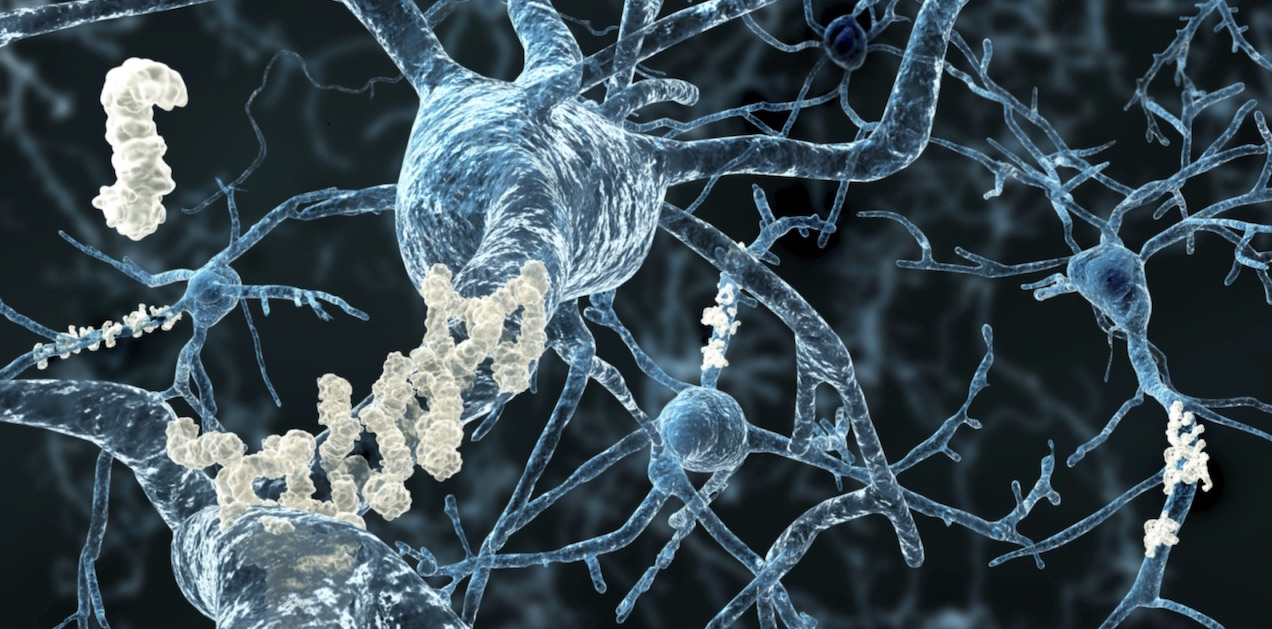
\includegraphics[width = 1 \textwidth]{Imagenes/Vectorial/proteina-tau.jpg}
	\caption{Clogging of neurons by vitamin tau \citep{tau}}
	\label{fig:tau}
\end{figure}


\section{Reminiscence therapy}

Fortunately, there are therapies that help improve the quality of life of people who suffer from this disease. Among them cognitive stimulation, reality orientation, therapeutic exercise, music therapy, and multisensory stimulation, among others \citep{SAS2020}.\\

Our project is linked to reminiscence therapy, which is a process that helps the person evoke emotional moments and experiences and integrate them into the present, which can improve self-esteem and quality of life \citep{gonzalez2015terapia}.\\

Specifically, the technique consists of showing the person a visual, musical or even olfactory tool or material, linked to their own experience or historical facts. In this way, a review of the person's life will be promoted, so that a connection is achieved with their experiences, in order to reconstruct a life book and reinforce their identity as a person.   This therapy can be classified as a type of daydreaming that takes them to their past, allowing them to enter a state of concentration in order to strengthen their general memory, which strengthens the brain and develops their social abilities, stimulates memories. through sensory organs and activates their sense of identity.\\



Some of the benefits of life book creation and reminiscence occupational therapy, among many others, are:\\
\begin{itemize}
	\item \underline{Emotional well-being}: It allows people to remember positive and significant experiences in their lives, which can generate satisfactory feelings of joy and happiness.\\
	\ item \ underline {Self-knowledge}: When a person reviews and reflects on past events and personal achievements, he can gain an understanding of himself. Through the interaction of his memories, aided by the guidance of caregivers and therapists, he is able to evoke aspects of his values, strengths and weaknesses that would not otherwise be accessible.
	\item \underline{Personal meaning and purpose}: By recalling significant scenes, people can find emotional guidance that allows them to give meaning and direction to their lives, especially in times of confusion or disorientation.
	\item \underline{Stress reduction}: By focusing on positive memories, people experience a sense of calm, tranquility and emotional well-being, and find a space to escape the stress and tensions of the present.
	\item \underline{Promote social relationships}: Sharing memories and experiences with other people can strengthen social ties and foster a greater connection with caregivers, family and friends, which is highly satisfactory for the patient.
	\item \underline{Increase language and person development}: By recounting past experiences, people improve their ability to communicate effectively as well as their verbal expression, which drives significant emotional and intellectual personal growth.
	\item \underline{Prevent disability}: Strengthening language skills and keeping the mind active can help preserve cognitive function over time. 
	\end{itemize}
	
	
	
	In summary, it is recommended to carry out occupational therapy activities because they improve the quality of life of patients, because personal and life satisfaction is achieved, attention, memory and language are stimulated, moments are relived. meaningful and emotional and socialization is encouraged. All of this leads to delaying possible cognitive problems \citep{SAS2020}.\\
	
	\section{About the project}
	
	Given these benefits, the initiative to carry out this project was born, as it is a visual support tool for the narration of life books. A life book is a compilation of the most important and characteristic events of a person throughout their life, adding visual support and usually being organized by stages. The characteristic of a life book is to give a context to the incorporated images so that what has been experienced can be understood in a timeline, which helps to enhance the person's memory and their sense of identity \citep{life book }. 
	
	To create it, we will use artificial intelligence techniques that convert text inputs to images and in this way, we will be able to transform memories narrated by the patient and convert them into images that correspond to the memory described. The interesting thing is to be able to give the possibility of making these images more personal so that a series of images of one's own, of family members or of important events in the patient's life can be added, to train the generative artificial intelligence model in charge of carrying out the process. of creating the images, and that the final result is unique, special and of great help to the person who suffers from this disease. 
	
	The work was born based on the CANTOR project (Automatic Composition of Personal Narratives to support Occupational Therapy based on Reminiscence, National Research Plan), an initiative proposed by researchers from a group of Spanish universities, including the Complutense University of Madrid.
	
	The main motivation for the creation of this project is to provide the possibility for patients with dementia caused by Alzheimer's to build a book made up of their happiest memories, giving them the opportunity to remember them. It has been shown that when patients talk about certain times in their lives and moments experienced in the past, a positive impact is generated on them, increasing their confidence and identity \citep{UCMcantor}.\\
	
The CANTOR project is designed to be carried out in two stages: 
\begin{itemize}
	\item The first would be the technical part in which a tool is developed to automate the construction of the life book using artificial intelligence. 
	\item The second stage consists of taking the tool to the therapists and people who assist those affected to check its functionality and effectiveness. 
\end{itemize}

We will focus on addressing the first stage of the project, making sure to implement a tool capable of generating images through an artificial intelligence technique specialized in this, in a way that ensures the maximum possible quality in the results and ensuring a practically total resemblance to reality. That is, our objective is to create a tool that is capable of helping in the process of reminiscence therapy for the creation of a life book of a certain patient, so that visual representations can be created from descriptions that the person contribution of certain memories. The usefulness and purpose of creating images from text using a trained artificial intelligence technique is to obtain personal images to remember moments in your life that are not immortalized in a photograph or that you do not have access to. \\

For it to be possible to generate personal images through artificial intelligence methods, it is necessary for family members to provide a sufficiently large number of photographs of the patient at different stages of their life (minimum 10 of each), or of people, places, animals or objects that may be meaningful to him or her. The purpose is to teach the artificial intelligence model designed to generate images to identify the desired element. And thus, obtaining as a result a personalized image of the person to serve as support in reminiscence therapy, to be included in the person's life book and to generate a positive impact on their mental well-being \\.


\section{Goals}

For the correct completion of the project and in order to obtain the best possible results, we have established some objectives to guide us during the preparation of the work and keep in mind at all times the path we will take to carry it out. 

\begin{itemize}
	\item Study the different artificial intelligence techniques in order to choose the most appropriate one for generating images. 
	\item Analyze the necessary characteristics of the input data set for effective training of the artificial intelligence model. 
	\item Use generative artificial intelligence to create personal images that help patients evoke emotional moments and experiences and integrate them into the present.
	\item Generate photographs that support patient stories for the creation of a life book.
	\item Provide support material for reminiscence therapy.
	\item Develop a program through which an assistant can incorporate his or her own images into a life book. 
	
\end{itemize} 

For example: a patient remembers when she saw the sea for the first time, but does not know enough details to have a story integrated into her mind, nor did he take any photographs at that time. The model can generate a photo of the patient at sea, and the fact of evoking that memory causes well-being and happiness.

In this way, we can provide very valuable material for reminiscence therapy, since visual material is needed to create a connection with the patient's life, and this material can sometimes be very limited.


\section{Work plan}

Once the objectives have been defined, a method must be established to try to achieve the expected results. First of all, extensive research must be carried out about the different artificial intelligence techniques that exist and which of them all best adapts to our object of study. But before delving into the different techniques and models, we must be aware of the reason why we do this work, that is, who the recipient is and what they expect from the final product. Therefore, we need to investigate the focus of the problem and know how artificial intelligence can help solve it, or mitigate it. 

To obtain the desired results we need to know what the best techniques are at our disposal, and if we can use them and work on them. Therefore, an important part of our project consists of testing each of them and assessing which one generates images of higher quality and in an acceptable time. It is necessary to test each and every one that is available, and know what our execution environment is going to be.

Once we have decided which model or models we will choose to develop our project, the time will come to know how we are going to deploy the different technologies and what we are going to add to make it something useful and completely new for our recipients. The idea is to create a program that contains the chosen artificial intelligence model and a simple and effective interface to use it in occupational therapies. In addition, these models must have the possibility of being customizable, so that images can be created with the elements or people you want. To do this, we will investigate the different training modes, and by carrying out multiple tests and analyzing the different results, we will reason which will be the training with the best time and quality within our possibilities for the project.

When we already have an image-generative artificial intelligence model that provides good results, we will simulate use cases that exemplify how users can have a satisfactory experience. As a result of this, we will be able to obtain a series of conclusions and note whether expectations have been met, in addition to evaluating whether the initiative and the work carried out could be useful to improve the quality of life of patients.
\chapter*{Conclusions and Future Work}
\label{cap:conclusions}
\addcontentsline{toc}{chapter}{Conclusions and Future Work}
\subsection{Conclusions}

First of all, we can affirm that, through the help of artificial intelligence, personalized photographic material can be provided that can be used to collaborate with occupational therapies, so that a patient has the possibility of evoking significant moments, which they would not otherwise have. the ability to visualize.\\

With respect to image generation, the objective of training an artificial intelligence model to convert text to image has been achieved, including the person considered. This fact means that, in reminiscence therapy, if we are given a considerable number of images in which a specific person appears (from ten), we can work based on a trained model that recognizes that person, and generate the desired images from it.\\

Additionally, the model that has been obtained can serve as a basis for carrying out new training, which fits perfectly with our objectives, since for a certain patient, we can develop a large model that includes the desired number of people. . However, Stable Diffusion and its derived models have a limitation, since the same image is difficult to generate with multiple elements. We have achieved acceptable results on some occasions with a considerable number of steps, but it requires a lot of patience and we cannot guarantee absolute success, as we can in a generation with a main element.\\

Another important aspect that we must take into account and that we have reached the conclusion after all the research, is that to make our model work, like any other image-generative artificial intelligence, a large capacity of graphic memory is needed. . With our team's GPU, the generation will always last a few minutes, and the more quality desired, the longer the time will increase. This is a fact that all people who provide the service of generating personalized photographs must know.\\

Regarding the training of the models, we can conclude that the number of steps with which it is performed correctly is 2400 for a training of 10 images, since multiple tests have been carried out with more steps, in which overtraining is detected, and with fewer steps, in which a lack of training is detected.\\

Based on the results obtained, we can affirm that the training that maximizes the quality of the images is that of Dreambooth, with a quality higher than that achieved with LoRA. With this last model, it was much more difficult to obtain personalized images from the trained element, since given its characteristics, it focused on displaying only the element, ignoring the complements that were requested in the prompt. Through Dreambooth, the images showed superior quality and everything that was requested in the description of the photograph was reflected. With both training models, we can conclude that all types of elements can be trained, whether people, animals or places, since correct results have been obtained with all of them.\\

Regarding the application, we have managed to create a program through which personalized photographs can be generated from our trained models. This produces very good results and also allows the visualization of a life book based on a story created by us. The idea is that a user can have a program with which they can generate personalized images and develop a very attractive life book in a simple way.\\

We can conclude that we have met the objectives we had previously at the beginning of this project, since we have built a program through which a user could obtain personalized images with a reasonable quality in an adequate time. There has been a constant evolution in recent months in which we went from not being able to generate images locally, to being able to generate them with trained models, and then being able to display those photographs in an application developed by us.\\

\subsection{Future work}

After carrying out this project, we would like people in charge of assisting patients with memory loss to be able to carry out research based on our model, with the aim of psychologically studying to what extent the reduction of stress is being promoted, is being enhanced. the patient's cognitive capacity and people's satisfaction is being achieved. This is the greatest objective we have with this artificial intelligence, to achieve personal well-being, and the scope of this work does not allow us to verify if we have really obtained great results in the social aspect.\\

Additionally, it would be convenient that if this project were used by therapists, they should have a computer with a large graphics card, so that as little time as possible would be invested in generating the images. After having used this same model in the cloud, where they use servers with high-power GPUs, obtaining results was instantaneous, which is why we highlight a large margin for improvement that, if reduced, will greatly speed up the therapy. Furthermore, it should be noted that in our model, we have used version 1.5 of Stable Diffusion because it is the only one that could work locally with our team's graphics card. With an improvement in this aspect, the XL version could be worked on and trained, which provides great quality to the images, and even better results would be achieved by minimizing the waiting time. In addition, Stable Diffusion has recently released a new version 3 that ensures speed, efficiency and quality in the images generated without needing to use as much space as the XL version, so it would be a very attractive option to work with. You could even take the work of life books one step further and generate small video clips that better represent the latest developments that large Artificial Intelligence companies such as OpenAI through Sora and Stable Diffusion are including. via Stable Diffusion Video. They are technologies that produce impressive results but that are not currently available to users but we hope that they will be in the not too distant future. \\

Regarding the training of images with Stable Diffusion, as proposals for improvement we would like to find an optimal way to include several tokens that represent trained elements in the same image and that it is not necessary to resort to the inpainting technique. Methods could be tested such as training more images of both elements in the same training stage and that they can be included under the same token, although the behavior that the model could have in terms of results is uncertain, multilayers are an interesting concept in terms of generation of images for life books. \\

Based on having made an application that tests the trained models and displays a life book with personalized images, we would like to implement a server so that performance depends exclusively on it and the internet connection, and not on the computer. of each user and their graphics card. In this way, strong utilization requirements would be eliminated. Furthermore, it would be convenient to continue developing this program, allowing users to register and manage the life book of reminiscence therapy patients. To carry out this proposal, the project would have to be connected to a database that contains the user registry, and within each of them, a table with the patient's life book, which should have as attributes, mainly, an image, a title and a description. We believe that it can be an attractive format for therapy, where users can very easily personalize a life book, with real images, or those created by artificial intelligence, in the event that there are no graphic documents of a relevant fact, meaningful and emotional for the patient's life.


\end{otherlanguage}
%%%%%%%%%%%%%%%%%%%%%%%%%%%%%%%%%%%%%%%%%%%%%%%%%%%%%%%%%%%%%%%%%%%%%%%%%%%

\chapter*{Contribuciones Personales}
\label{cap:contribucionesPersonales}
\addcontentsline{toc}{chapter}{Contribuciones Personales}
\section*{Estudiante 1: Sergio Llorente Hernando}

Lo primero de todo fue reflexionar sobre los objetivos del proyecto, de manera que realicé una investigación sobre la terapia ocupacional, los libros de vida y las distintas inteligencias artificiales, con el objetivo de saber qué tecnología debemos utilizar para satisfacer las necesidades de los usuarios.\\

Desde un primer momento hice una labor de búsqueda y prueba de diferentes modelos de inteligencia artificial generativa de imágenes. En primer lugar, la prueba era con servidores especializados y más adelante, hice una descarga de los modelos que generaban imágenes de calidad, con el objetivo de comprobar cuáles de los modelos podrían funcionar mejor y otorgar unos resultados satisfactorios.\\

El siguiente paso en el que me centré fue en conseguir hacer funcionar la inteligencia artificial generativa en local. Para ello, en primer lugar opté por probar los modelos en anaconda, lo cual no era una interfaz cómoda para el usuario y la generación de imágenes era lenta. A continuación empecé a trabajar con SDGUI, una aplicación con la que podía testar cualquier tipo de modelo, ya sea entrenado o no, y además de eso, ajustar todos los parámetros necesarios. Con esta aplicación sí que se generaban bien las imágenes. Esto sirvió para diseñar nuestro propio programa que incluyera el modelo generativo. \\

Para crear la aplicación, primero opté por crear un script de Python. Esto dio buenos resultados, porque mostraba la imagen al igual que en el programa de referencia, pero la interfaz no era buena para el usuario, y además haciendo pruebas en cualquier otro ordenador no obtuve resultados. Este hecho hizo que creara un entorno virtual para saber las dependencias que son necesarias para que funcione el modelo, y por otro lado, dividir el back y el front, con el objetivo de hacer más atractiva la aplicación mediante html, que es un lenguaje con el que ya estaba más familiarizado. Esto dio un mejor resultado, y se consiguió generar imágenes en una aplicación con una buena interfaz y un buen diseño.\\

La siguiente fase del trabajo, fue la del entrenamiento de los modelos, con el objetivo de tener la capacidad de personalizar la inteligencia artificial a petición de cualquier usuario. Fue un trabajo muy complejo en el que hice muchísimas pruebas con diferentes vías, con el objetivo de obtener los mejores resultados posibles. Fueron múltiples pruebas debido a que, para ofrecer al usuario la experiencia óptima, necesitamos conocer cuántas imágenes y cuántos pasos de aprendizaje se requieren. Tras la realización de estas pruebas se concluyó que la estrategia más óptima era utilizar un conjunto de 10 imágenes y 2400 pasos de entrenamiento. No obstante, hicieron falta múltiples entrenamientos erróneos o parcialmente correctos para conocer este hecho. \\

La siguiente fase fue realizar más entrenamientos con diferentes elementos y analizar los resultados. Además, aquí opté por examinar si un resultado de un entrenamiento podía servir de base para un próximo. La respuesta fue afirmativa y eso me llevó a añadir múltiples capas a un mismo modelo, lo cual podría ayudar a un usuario a tener un solo modelo personalizado que incluya todos los elementos que desee. \\

Por último, traté de lograr que la aplicación generase imágenes mediante modelos entrenados por nosotros mismos. Fue una fase complicada, pero finalmente se logró un resultado satisfactorio. Además, al entorno de la aplicación le añadí una página que representa un ejemplo de libro de vida desarrollado por nosotros, con unas imágenes generadas por nuestra aplicación. De esta manera, tenemos una aplicación con dos páginas. Una que muestra el tipo de libros de vida que podríamos desarrollar, y una que es un entorno de generación de imágenes con múltiples modelos y de diferentes maneras.


\section*{Estudiante 2: Isabella Romano Ramos}
Lo primero que realicé fue la introducción del tema de estudio sobre el trabajo después de la primera sesión de reunión con el tutor en la que quedaron claros los aspectos generales que se iban a abordar, los objetivos principales y las tecnologías que se iban a utilizar. \\

Una vez definido esto, empezó la fase de investigación sobre los temas principales que abordaban el proyecto: el Alzheimer y la Inteligencia Artificial. Me embarqué en un proceso de recopilación de información para entender lo que ocurre en el cerebro que hace que se deteriore la memoria y que cause esta enfermedad que afecta a millones de personas, y así poder reflejarlo en la memoria. En cuanto a la IA, era un concepto totalmente nuevo para mí ya que no había visto nada sobre este campo en ninguna asignatura de la carrera. Por lo que opté empezar a entenderla por el principio, desde un concepto tan simple como el perceptrón, hasta examinar las redes neuronales, pasando por todos los tipos de modelos fundamentales qué existen y saber diferenciar la función de cada uno. Por ende, me encargué de buscar la bibliografía que hablaba de la IA, más en concreto sobre el Deep Learning y las redes neuronales. De esta manera, lo pude redactar de manera que se entendiera lo mejor posible en el Capítulo 2 Estado de la cuestión. \\

Como se ha podido ver a lo largo de todo el proyecto, nos hemos centrado en el campo concreto de la Inteligencia Artificial generativa de imágenes y lo que hicé fue investigar las diferentes alternativas de modelos ya implementados que pudiéramos utilizar para el entrenamiento de personas y la integración en nuestra futura aplicación. Tras examinar profundamente las prestaciones y disponibilidad de cada uno, entre los tres candidatos finales, que se trataban de Midjourney, Dall-e y Stable Diffusion, se eligió usar el último por las limitaciones que nos mostraban los otros dos modelos. Una vez elegido, hice un análisis profundo de cómo está implementado el modelo de difusión estable que utiliza la herramienta y lo redacté extensamente en el Capítulo 2 Estado de la cuestión. Además, durante el proceso surgieron conceptos interesantes en relación con Stable Diffusion, como LORA y Dreambooth e incluso, consideré importante añadir la importancia de la ingeniería del prompt para la creación de imágenes a partir de texto. \\

Cuando pude comprender los conceptos teóricos que explicaban el funcionamiento de Stable Diffusion, se pasó a la parte práctica, es decir, a pensar en la estructura y usos de la aplicación que se iba a desarrollar como apoyo al modelo de IA generativa seleccionado. Finalmente, caímos en la cuenta de que las prestaciones que ofrecen mis dos equipos, tanto mi portatil como el ordenador de sobremesa, no cumplen los requisitos mínimos para poder ejecutar la aplicación en local ni realizar las pruebas necesarias sobre la generación de imágenes, al no contar con GPU en el portátil y no ser lo suficientemente potente la GPU en el ordenador de sobremesa. Es decir, era inviable que se pudieran generar imágenes en mis equipos.\\

Por ello, solo me podía limitar a entrenar el modelo que seleccionamos a través de la herramienta de Google Colab. Fue entonces cuando busqué en Hugging Face el modelo de Stable Diffusion más adecuado, que resultó ser el 1.5, y fui probando el número de pasos y de imágenes que producían los mejores resultados. \\

El c


Además, me encargué de organizar y estructurar el contenido de la memoria en la herramienta de Latex, utilizada para generar este mismo documento. \\




%
% Bibliografía
%
% Si el TFM se escribe en inglés, editar TeXiS/TeXiS_bib para cambiar el
% estilo de las referencias
%---------------------------------------------------------------------
%
%                      configBibliografia.tex
%
%---------------------------------------------------------------------
%
% bibliografia.tex
% Copyright 2009 Marco Antonio Gomez-Martin, Pedro Pablo Gomez-Martin
%
% This file belongs to the TeXiS manual, a LaTeX template for writting
% Thesis and other documents. The complete last TeXiS package can
% be obtained from http://gaia.fdi.ucm.es/projects/texis/
%
% Although the TeXiS template itself is distributed under the 
% conditions of the LaTeX Project Public License
% (http://www.latex-project.org/lppl.txt), the manual content
% uses the CC-BY-SA license that stays that you are free:
%
%    - to share & to copy, distribute and transmit the work
%    - to remix and to adapt the work
%
% under the following conditions:
%
%    - Attribution: you must attribute the work in the manner
%      specified by the author or licensor (but not in any way that
%      suggests that they endorse you or your use of the work).
%    - Share Alike: if you alter, transform, or build upon this
%      work, you may distribute the resulting work only under the
%      same, similar or a compatible license.
%
% The complete license is available in
% http://creativecommons.org/licenses/by-sa/3.0/legalcode
%
%---------------------------------------------------------------------
%
% Fichero  que  configura  los  parámetros  de  la  generación  de  la
% bibliografía.  Existen dos  parámetros configurables:  los ficheros
% .bib que se utilizan y la frase célebre que aparece justo antes de la
% primera referencia.
%
%---------------------------------------------------------------------


%%%%%%%%%%%%%%%%%%%%%%%%%%%%%%%%%%%%%%%%%%%%%%%%%%%%%%%%%%%%%%%%%%%%%%
% Definición de los ficheros .bib utilizados:
% \setBibFiles{<lista ficheros sin extension, separados por comas>}
% Nota:
% Es IMPORTANTE que los ficheros estén en la misma línea que
% el comando \setBibFiles. Si se desea utilizar varias líneas,
% terminarlas con una apertura de comentario.
%%%%%%%%%%%%%%%%%%%%%%%%%%%%%%%%%%%%%%%%%%%%%%%%%%%%%%%%%%%%%%%%%%%%%%
\setBibFiles{%
biblio%
}

%%%%%%%%%%%%%%%%%%%%%%%%%%%%%%%%%%%%%%%%%%%%%%%%%%%%%%%%%%%%%%%%%%%%%%
% Definición de la frase célebre para el capítulo de la
% bibliografía. Dentro normalmente se querrá hacer uso del entorno
% \begin{FraseCelebre}, que contendrá a su vez otros dos entornos,
% un \begin{Frase} y un \begin{Fuente}.
%
% Nota:
% Si no se quiere cita, se puede eliminar su definición (en la
% macro setCitaBibliografia{} ).
%%%%%%%%%%%%%%%%%%%%%%%%%%%%%%%%%%%%%%%%%%%%%%%%%%%%%%%%%%%%%%%%%%%%%%
\setCitaBibliografia{
\begin{FraseCelebre}
\begin{Frase}
  Y así, del mucho leer y del poco dormir, se le secó el celebro de
  manera que vino a perder el juicio.\\ 
  \textcolor{red}{(modificar en Cascaras$\backslash$bibliografia.tex)}
\end{Frase}
\begin{Fuente}
  Miguel de Cervantes Saavedra
\end{Fuente}
\end{FraseCelebre}
}

%%
%% Creamos la bibliografia
%%
\makeBib

% Variable local para emacs, para  que encuentre el fichero maestro de
% compilación y funcionen mejor algunas teclas rápidas de AucTeX

%%%
%%% Local Variables:
%%% mode: latex
%%% TeX-master: "../Tesis.tex"
%%% End:



% Apéndices
\appendix
\chapter{Título del Apéndice A}
\label{Appendix:Key1}

Los apéndices son secciones al final del documento en las que se agrega texto con el objetivo de ampliar los contenidos del documento principal.
\chapter{Título del Apéndice B}
\label{Appendix:Key2}

Se pueden añadir los apéndices que se consideren oportunos.
%\include{Apendices/appendixC}
%\include{...}
%\include{...}
%\include{...}
\backmatter



%
% Índice de palabras
%

% Sólo  la   generamos  si  está   declarada  \generaindice.  Consulta
% TeXiS.sty para más información.

% En realidad, el soporte para la generación de índices de palabras
% en TeXiS no está documentada en el manual, porque no ha sido usada
% "en producción". Por tanto, el fichero que genera el índice
% *no* se incluye aquí (está comentado). Consulta la documentación
% en TeXiS_pream.tex para más información.
\ifx\generaindice\undefined
\else
%%---------------------------------------------------------------------
%
%                        TeXiS_indice.tex
%
%---------------------------------------------------------------------
%
% TeXiS_indice.tex
% Copyright 2009 Marco Antonio Gomez-Martin, Pedro Pablo Gomez-Martin
%
% This file belongs to TeXiS, a LaTeX template for writting
% Thesis and other documents. The complete last TeXiS package can
% be obtained from http://gaia.fdi.ucm.es/projects/texis/
%
% This work may be distributed and/or modified under the
% conditions of the LaTeX Project Public License, either version 1.3
% of this license or (at your option) any later version.
% The latest version of this license is in
%   http://www.latex-project.org/lppl.txt
% and version 1.3 or later is part of all distributions of LaTeX
% version 2005/12/01 or later.
%
% This work has the LPPL maintenance status `maintained'.
% 
% The Current Maintainers of this work are Marco Antonio Gomez-Martin
% and Pedro Pablo Gomez-Martin
%
%---------------------------------------------------------------------
%
% Contiene  los  comandos  para  generar  el índice  de  palabras  del
% documento.
%
%---------------------------------------------------------------------
%
% NOTA IMPORTANTE: el  soporte en TeXiS para el  índice de palabras es
% embrionario, y  de hecho  ni siquiera se  describe en el  manual. Se
% proporciona  una infraestructura  básica (sin  terminar)  para ello,
% pero  no ha  sido usada  "en producción".  De hecho,  a pesar  de la
% existencia de  este fichero, *no* se incluye  en Tesis.tex. Consulta
% la documentación en TeXiS_pream.tex para más información.
%
%---------------------------------------------------------------------


% Si se  va a generar  la tabla de  contenidos (el índice  habitual) y
% también vamos a  generar el índice de palabras  (ambas decisiones se
% toman en  función de  la definición  o no de  un par  de constantes,
% puedes consultar modo.tex para más información), entonces metemos en
% la tabla de contenidos una  entrada para marcar la página donde está
% el índice de palabras.

\ifx\generatoc\undefined
\else
   \addcontentsline{toc}{chapter}{\indexname}
\fi


% Generamos el índice
\printindex

% Variable local para emacs, para  que encuentre el fichero maestro de
% compilación y funcionen mejor algunas teclas rápidas de AucTeX

%%%
%%% Local Variables:
%%% mode: latex
%%% TeX-master: "./tesis.tex"
%%% End:

\fi

%
% Lista de acrónimos
%

% Sólo  lo  generamos  si  está declarada  \generaacronimos.  Consulta
% TeXiS.sty para más información.


\ifx\generaacronimos\undefined
\else
%---------------------------------------------------------------------
%
%                        TeXiS_acron.tex
%
%---------------------------------------------------------------------
%
% TeXiS_acron.tex
% Copyright 2009 Marco Antonio Gomez-Martin, Pedro Pablo Gomez-Martin
%
% This file belongs to TeXiS, a LaTeX template for writting
% Thesis and other documents. The complete last TeXiS package can
% be obtained from http://gaia.fdi.ucm.es/projects/texis/
%
% This work may be distributed and/or modified under the
% conditions of the LaTeX Project Public License, either version 1.3
% of this license or (at your option) any later version.
% The latest version of this license is in
%   http://www.latex-project.org/lppl.txt
% and version 1.3 or later is part of all distributions of LaTeX
% version 2005/12/01 or later.
%
% This work has the LPPL maintenance status `maintained'.
% 
% The Current Maintainers of this work are Marco Antonio Gomez-Martin
% and Pedro Pablo Gomez-Martin
%
%---------------------------------------------------------------------
%
% Contiene  los  comandos  para  generar  el listado de acrónimos
% documento.
%
%---------------------------------------------------------------------
%
% NOTA IMPORTANTE:  para que la  generación de acrónimos  funcione, al
% menos  debe  existir  un  acrónimo   en  el  documento.  Si  no,  la
% compilación  del   fichero  LaTeX  falla  con   un  error  "extraño"
% (indicando  que  quizá  falte  un \item).   Consulta  el  comentario
% referente al paquete glosstex en TeXiS_pream.tex.
%
%---------------------------------------------------------------------


% Redefinimos a español  el título de la lista  de acrónimos (Babel no
% lo hace por nosotros esta vez)

\def\listacronymname{Lista de acrónimos}

% Para el glosario:
% \def\glosarryname{Glosario}

% Si se  va a generar  la tabla de  contenidos (el índice  habitual) y
% también vamos a  generar la lista de acrónimos  (ambas decisiones se
% toman en  función de  la definición  o no de  un par  de constantes,
% puedes consultar config.tex  para más información), entonces metemos
% en la  tabla de contenidos una  entrada para marcar  la página donde
% está el índice de palabras.

\ifx\generatoc\undefined
\else
   \addcontentsline{toc}{chapter}{\listacronymname}
\fi


% Generamos la lista de acrónimos (en realidad el índice asociado a la
% lista "acr" de GlossTeX)

\printglosstex(acr)

% Variable local para emacs, para  que encuentre el fichero maestro de
% compilación y funcionen mejor algunas teclas rápidas de AucTeX

%%%
%%% Local Variables:
%%% mode: latex
%%% TeX-master: "../Tesis.tex"
%%% End:

\fi

%
% Final
%
%---------------------------------------------------------------------
%
%                      fin.tex
%
%---------------------------------------------------------------------
%
% fin.tex
% Copyright 2009 Marco Antonio Gomez-Martin, Pedro Pablo Gomez-Martin
%
% This file belongs to the TeXiS manual, a LaTeX template for writting
% Thesis and other documents. The complete last TeXiS package can
% be obtained from http://gaia.fdi.ucm.es/projects/texis/
%
% Although the TeXiS template itself is distributed under the 
% conditions of the LaTeX Project Public License
% (http://www.latex-project.org/lppl.txt), the manual content
% uses the CC-BY-SA license that stays that you are free:
%
%    - to share & to copy, distribute and transmit the work
%    - to remix and to adapt the work
%
% under the following conditions:
%
%    - Attribution: you must attribute the work in the manner
%      specified by the author or licensor (but not in any way that
%      suggests that they endorse you or your use of the work).
%    - Share Alike: if you alter, transform, or build upon this
%      work, you may distribute the resulting work only under the
%      same, similar or a compatible license.
%
% The complete license is available in
% http://creativecommons.org/licenses/by-sa/3.0/legalcode
%
%---------------------------------------------------------------------
%
% Contiene la última página
%
%---------------------------------------------------------------------


% Ponemos el marcador en el PDF
\ifpdf
   \pdfbookmark{Fin}{fin}
\fi

\thispagestyle{empty}\mbox{}

Este texto se puede encontrar en el fichero Cascaras/fin.tex. Si deseas eliminarlo, basta con comentar la línea correspondiente al final del fichero TFGTeXiS.tex.

\vspace*{4cm}

\small

\hfill \emph{--¿Qué te parece desto, Sancho? -- Dijo Don Quijote --}

\hfill \emph{Bien podrán los encantadores quitarme la ventura,}

\hfill \emph{pero el esfuerzo y el ánimo, será imposible.}

\hfill 

\hfill \emph{Segunda parte del Ingenioso Caballero} 

\hfill \emph{Don Quijote de la Mancha}

\hfill \emph{Miguel de Cervantes}

\vfill%space*{4cm}

\hfill \emph{--Buena está -- dijo Sancho --; fírmela vuestra merced.}

\hfill \emph{--No es menester firmarla -- dijo Don Quijote--,}

\hfill \emph{sino solamente poner mi rúbrica.}

\hfill 

\hfill \emph{Primera parte del Ingenioso Caballero} 

\hfill \emph{Don Quijote de la Mancha}

\hfill \emph{Miguel de Cervantes}


\newpage
\thispagestyle{empty}\mbox{}

\newpage

% Variable local para emacs, para  que encuentre el fichero maestro de
% compilación y funcionen mejor algunas teclas rápidas de AucTeX

%%%
%%% Local Variables:
%%% mode: latex
%%% TeX-master: "../Tesis.tex"
%%% End:

%\end{otherlanguage}
\end{document}
